%!TEX program = xelatex
% 최종 보고서 (백로그 14). 뼈대와 절별 출처는 docs/final_outline.md
%
% 본문은 paper/sections/ 에 장별로 나누어 둔다. 한 파일이 커지면 고칠 때
% 어디를 보는지 헷갈리고, 장 단위로 다시 쓰기도 어렵기 때문이다.
%
% 서술 규칙: 모든 효과는 반사실 대비로 (결정기록 0006), 숫자에는 조건을
% (0007). 표는 scripts/build_tables.py 가 결과 JSON 에서 만든다 — 손으로
% 고치지 않는다. 그림은 복사하지 않고 ../output/figures 를 그대로 본다.
%
% 빌드:  .\paper\build.ps1

\documentclass[11pt, a4paper]{article}

% ─── Packages ────────────────────────────────────────────────────────────────
\usepackage{fontspec}
\usepackage{kotex}
\usepackage[margin=2.5cm]{geometry}
\usepackage{amsmath, amssymb, bm}
\usepackage{graphicx}
\usepackage{booktabs}
\usepackage{multirow}
\usepackage{array}
\usepackage{xcolor}
\usepackage{hyperref}
\usepackage{natbib}
\usepackage{caption}
\usepackage{subcaption}
\usepackage{float}
\usepackage[section]{placeins}
\usepackage{enumitem}
\usepackage{parskip}
\usepackage{titlesec}
\usepackage{setspace}

% Malgun Gothic 에는 이탤릭이 없어 \emph 를 한글에 쓰면 'Font shape ... /it
% undefined' 경고가 나고 모양이 정의되지 않은 채 조판된다. 기울임을 만들어
% 준다 — 한글 \emph 가 본문에 여럿 있고 전부 의도적인 강조다.
\setmainhangulfont{Malgun Gothic}[AutoFakeSlant=0.167]
\setsanshangulfont{Malgun Gothic}[AutoFakeSlant=0.167]
\setmonohangulfont{Malgun Gothic}

\onehalfspacing
\setlength{\parindent}{0pt}
\setlength{\parskip}{6pt}

% article 클래스의 영어 이름을 한글로. kotex 만으로는 안 바뀐다.
\renewcommand{\tablename}{표}
\renewcommand{\figurename}{그림}
\renewcommand{\contentsname}{차례}
\renewcommand{\listfigurename}{그림 차례}
\renewcommand{\listtablename}{표 차례}
\renewcommand{\abstractname}{초록}
\renewcommand{\refname}{참고문헌}
\renewcommand{\bibname}{참고문헌}
\renewcommand{\appendixname}{부록}
\captionsetup{labelsep=period}

\hypersetup{
    colorlinks=true,
    linkcolor=blue!60!black,
    citecolor=green!50!black,
    urlcolor=blue!70!black
}

\graphicspath{{figures/}{../output/figures/}}

% 단계 수 매크로(\pipeSteps 등). scripts/plot_pipeline.py 가 run_all.py 의
% 단계 표에서 세어 만든다 — 주차 보고서가 늘면 단계도 늘므로 손으로 적으면
% 바로 유령 숫자가 된다(3.7절).
% 이 파일은 scripts/plot_pipeline.py 가 만든다. 손으로 고치지 않는다.
% 단계 수는 run_all.py 의 STEPS 에서, 산출물 수는 실제 파일에서 센다.

\newcommand{\pipeSteps}{49}
\newcommand{\pipeStepsAll}{50}
\newcommand{\pipeData}{2}
\newcommand{\pipePolicy}{7}
\newcommand{\pipeAnalysis}{19}
\newcommand{\pipeReplicate}{2}
\newcommand{\pipeViz}{7}
\newcommand{\pipeDocs}{12}
\newcommand{\pipeResults}{25}
\newcommand{\pipeFigures}{24}
\newcommand{\pipeTables}{16}


% ─── Title ───────────────────────────────────────────────────────────────────
\title{
    \vspace{-1cm}
    {\large 캡스톤 디자인 프로젝트 --- 최종 보고서}\\[0.8em]
    \textbf{서울 아파트 실거래와 정책 공고를 결합한\\
    미시 패널 구축과\\
    토지거래허가구역 인과효과 추정}
}

\author{
    이찬희 (Lee Chanhee)\\
    컴퓨터공학부\\
    서울과학기술대학교\\
    \texttt{happilyfly@seoultech.ac.kr}
}

\date{2026년 11월}

\begin{document}

\maketitle
\thispagestyle{empty}

% 초록. 본문을 다 쓴 뒤 마지막에 손본다.

\begin{abstract}
본 보고서는 서울시 토지거래허가구역(이하 토허제) 지정이 아파트 \emph{거래량과
가격}에 미친 인과효과를 실거래 미시자료로 추정한다. 국토교통부 아파트 매매
실거래 \emph{상세} 자료 47만 건(분석 8개 자치구, 2006-01$\sim$2026-05)과 서울시보·
전자관보의 지정 공고 원문을 결합해 \textbf{거래 한 건마다 계약일·전용면적·층·단지
식별자와 그 시점의 규제 상태를 붙인 미시 패널}을 구축하고, 2020년 6월 지정,
2021년 4월 확대 지정, 2025년 2월 부분 해제와 3월 재지정을 사건으로 삼아
이중차분·사건연구·삼중차분·합성대조군으로 추정했다.

주요 발견은 넷이다.
(1) \textbf{지정 직후 3개월 거래량이 $-71 \sim -80\%$다.} 법정동 27개 가운데 4개를
처치로 고르는 모든 경우 17,550가지 중 진짜 배정이 1위이고, 사전 추세 위배를
실제 관측값의 1.6배까지 열어 두어도 구간이 0을 넘지 않으며, 합리적인 설계 조합
192가지가 전부 음수다. \textbf{열 달 뒤 완전히 다른 네 자치구에서 일어난
2021년 4월 지정에서도 같은 크기였고}, 두 사건의 차이는 0과 구분되지 않는다
($+8.7\%$, $p=0.715$).
(2) \textbf{선행연구끼리 결론이 엇갈린 이유는 지역 정의가 아니라 사건 시점
정렬이었다.} 설계 축별로 분해하면 사건 시점 정렬이 39.6\,\%p, 통제군 정의가
2.3\,\%p를 가른다. 달력 월로 자르면 $-40.5\%$, 효력일에 맞추면 $-80.1\%$다.
(3) \textbf{효과는 모두에게 같지 않았고, 그 차이는 대출 규제가 아니라 허가 대상의
면적 기준에서 왔다.} 2020년 지정은 대지 18\,m$^2$ 초과만 허가 대상이어서 소형은
거래가 줄지 않았고(전용 40\,m$^2$ 미만 $+125.7\%$), 2022년 6월 기준이 6\,m$^2$로
강화되자 \emph{그때} 소형만 33.2\% 줄었다. 기준을 바꾸지 않은 2021년 재지정에서는
소형이 움직이지 않았다($-8.1\%$, $p=0.61$). 이 메커니즘에서 세운
\textbf{사전 예측이 2025년 재지정 자료에서 확인됐다}(소형 $-71.5\%$).
(4) \textbf{가격을 잡았다는 증거는 약하다.} 평행추세를 가정하면 $-4 \sim -7\%$
(헤도닉+단지 $-5.9\%$, 반복매매 $-6.0\%$)이나, 그 가정을 조금만 풀면 0과
구분되지 않고(붕괴값 0.22) 합성대조군으로는 확인되지 않는다($p=0.511$).

\textbf{말할 수 없는 것도 적는다.} 효과가 얼마나 오래 가는지는 기준 분기 선택에
따라 $-20 \sim +16\%$로 흔들려 이 설계로 답할 수 없다. 부과와 해제의 대칭성도
가릴 수 없다. 일반화 범위는 두 사건·아홉 개 동이며 모두 서울 고가 재건축
지역이므로 \emph{서울 고가 재건축 지역에서는 일관된다}까지가 정확하다.

본 보고서의 또 하나의 축은 \textbf{분석의 전제가 되는 시스템}이다. 원자료 수집부터
그림·표 생성까지 \pipeSteps 단계 파이프라인 하나로 돌고, 문서 수치 검증·고아
산출물 점검·의존 점검·표 생성 넷이 매 실행마다 걸린다. 새 폴더에 내려받아 새 가상환경에서
돌려 결과 JSON 25개가 바이트 단위로 같은 것을 확인했다. 코드와 결정기록 \pipeDecisions 편
전체를 공개한다: \url{https://github.com/cosmicpotato2047/capstone-ltz-causal}.
\end{abstract}

\vspace{1em}
\noindent\textbf{키워드:} 토지거래허가구역, 이중차분, 사건연구, 미시 패널,
부동산 정책, 재현가능 연구

\vspace{1em}
\begin{center}\textbf{Abstract (English)}\end{center}
\small
This report estimates the causal effect of Seoul's Land Transaction Permit
Zones (LTZ) on apartment \emph{transaction volume and prices} using
transaction-level administrative data. We combine 472,782 detailed apartment
sale records (8 districts, 2006-01 to 2026-05) with the original designation
notices published in the Seoul and national gazettes, constructing a
\textbf{micro panel in which every transaction carries its contract date, floor
area, floor level, complex identifier, and the regulatory status in force on
that day}. Using the June 2020 designation, the April 2021 expansion, and the
February 2025 partial release followed by the March 2025 re-designation as
events, we estimate difference-in-differences, event-study, triple-difference,
and synthetic-control specifications.

Four findings.
(1) \textbf{Transaction volume falls by 71--80\% in the three months after
designation.} Among all 17{,}550 ways of drawing 4 treated neighbourhoods from
27, the true assignment ranks first; the result survives opening the
pre-trend violation to 1.6 times its observed magnitude
\citep{rambachan2023honest}; and all 192 reasonable specification combinations
are negative. \textbf{The April 2021 designation, ten months later and in four
entirely different districts, produced an effect of the same size}, and the
difference between the two events is indistinguishable from zero
($+8.7\%$, $p=0.715$).
(2) \textbf{Prior studies disagree because of event-time alignment, not
geography.} Decomposing by design axis, event-time alignment accounts for
39.6\,pp of the spread while the control-group definition accounts for 2.3\,pp.
Aligning on calendar months gives $-40.5\%$; aligning on the effective date
gives $-80.1\%$.
(3) \textbf{The effect was not uniform, and the heterogeneity came from the
permit-threshold floor area rather than from mortgage regulation.} Under the
2020 rule only lots above 18\,m$^2$ required a permit, so small units were
exempt and their transactions did not fall (units under 40\,m$^2$: $+125.7\%$).
When the threshold tightened to 6\,m$^2$ in June 2022, small units fell by
33.2\% \emph{at that moment}, while the 2021 re-designation, which left the
threshold unchanged, produced no movement ($-8.1\%$, $p=0.61$).
A \textbf{prediction registered from this mechanism was confirmed} in the 2025
re-designation (small units $-71.5\%$).
(4) \textbf{Evidence that prices were contained is weak.} Assuming parallel
trends gives $-4$ to $-7\%$, but relaxing that assumption slightly makes the
interval include zero (breakdown value 0.22) and the synthetic control does not
confirm it ($p=0.511$).

We also state what cannot be said: the duration of the effect swings between
$-20\%$ and $+16\%$ depending on the reference period, and the symmetry between
imposition and release cannot be resolved. External validity extends to two
events and nine neighbourhoods, all high-priced redevelopment areas in Seoul.

A second axis of this report is the \textbf{system that makes the analysis
possible}: a single \pipeSteps-step pipeline from data collection to figures and
tables, with automated checks for stale numbers in documents, orphaned
artefacts, dependency drift, and table generation. A clean-room reproduction in a fresh clone and
virtual environment produced 25 result files identical byte for byte. Code and
all \pipeDecisions{} decision records are public.
\normalsize


\newpage
\tableofcontents
% 표 39개·그림 18장이면 본문 차례만으로는 찾아가기 어렵다. \newpage 를 두면
% 차례가 한 줄 넘칠 때 거의 빈 쪽이 하나 생기므로 바로 잇는다.
\listoffigures
\listoftables
\newpage

% 1장 서론. 출처: docs/framing.md 1절 · docs/proposal.md

\section{서론}

\subsection{동기와 연구 질문}

토지거래허가제는 일정 면적을 넘는 토지 거래에 관할 구청장의 허가를 요구하는
제도다. 가격에 상한을 두지도, 세금을 매기지도 않는다. 거래 자체에 \textbf{허가
절차라는 마찰}을 붙일 뿐이다. 서울시는 2020년 6월 23일 국제교류복합지구 인근
네 개 법정동(대치·삼성·청담·잠실)을 지정했고, 2021년 4월 압구정·여의도·목동·성수로
넓혔으며, 2025년 2월 대부분을 해제했다가 39일 만에 더 넓게 재지정했다.

이 제도가 거래를 줄였다는 것은 새로운 발견이 아니다. 2020년 6월 지정을 다룬
국내 선행연구 세 편이 모두 ``거래 건수가 60\% 넘게 줄었다''고 이미 적었다
\citep{jeon2025, lee2025, yang2025}. 거래에 허가를 붙였으니 거래가 줄어드는 것은
제도의 정의에 가깝다. 그것만 확인하는 작업이라면 의미가 적다.

\textbf{이 연구가 묻는 것은 그다음이다.} 다섯 가지로 나눈다.

\begin{enumerate}[leftmargin=2em, itemsep=2pt]
  \item \textbf{얼마나} 줄었나 --- 선행연구의 60\%는 날짜를 달력 월로 세어
        지정 전 거래가 섞여 희석된 값일 수 있다.
  \item \textbf{언제까지} 갔나 --- 일시 충격인지 시장이 계속 얼어붙었는지에
        따라 정책의 비용이 다르다.
  \item \textbf{누구에게} 달랐나 --- 규제 설계의 어느 부분이 실제로 작동했는지.
  \item \textbf{어디로} 번졌나 --- 규제 밖 단지로 수요가 옮겨 갔다면 규제는
        문제를 푼 것이 아니라 옮긴 것이다.
  \item \textbf{가격은} 잡혔나 --- 토허제의 명분이 가격 안정이기 때문이다.
\end{enumerate}

이 다섯 질문에 대한 답을 미리 한 문장으로 요약하면 이렇다.
\textbf{토허제의 명분은 가격 안정인데 실제로 작동한 것은 거래 동결이었다. 거래는
확실하게 끊었지만 가격을 잡았다는 증거는 약하다.} 그리고 그 거래 동결조차
모두에게 같지 않았다 --- 허가 대상에서 빠진 소형 아파트는 오히려 거래가 늘었다.

\subsection{기여 사항}

\textbf{첫째, 거래 단위 미시 패널을 지었다.} 선행연구 세 편은 모두 동-월 집계
자료를 쓴다. 이 연구는 실거래 ``상세'' 자료로 거래 한 건마다 계약일, 전용면적,
층, 단지 식별자를 붙이고, 정책 공고 원문에서 읽은 지정 구간을 법정동별로 결합해
거래 시점의 규제 상태를 붙였다. 잘게 쪼갠 것 자체가 기여는 아니다. 기여는
\textbf{미시 자료가 아니면 보이지 않는 것을 보였다}는 데 있다(3장).

\textbf{둘째, 설계 선택이 결과를 가르는 정도를 정량화했다.} 합리적인 설계 조합
192가지를 전부 추정해, 선행연구끼리 결론이 엇갈린 이유가 ``지역을 어떻게
나눴느냐''(2.3\,\%p)가 아니라 ``사건 시점을 어디에 맞췄느냐''(39.6\,\%p)임을
보였다(2.4절).

\textbf{셋째, 효과의 이질성이 허가 대상의 면적 기준에서 왔음을 자연실험으로
갈랐다.} 처음에는 대출 규제가 원인이라고 보았으나 경계를 옮겨 보니 규제 문턱인
15억원에 계단이 없었다. 2022년 6월 허가 기준이 대지 18\,m$^2$에서 6\,m$^2$로
강화된 사건이 두 가설을 갈랐다(6장).

\textbf{넷째, 그 답으로 세운 예측이 다른 자료에서 확인됐다.} ``2025년 재지정은
면적 기준이 6\,m$^2$이므로 소형도 함께 줄어야 한다''고 미리 적었고, 실제로 소형
거래가 71.5\% 줄었다(6.8절). 그리고 2021년 4월 지정이라는 별개 사건에서 같은
크기의 효과가 나왔다(9.6절).

\textbf{다섯째, 전 과정을 공개하고 클린 환경에서 재현을 확인했다.} 원자료 수집부터
그림과 표 생성까지 \pipeSteps 단계 파이프라인 하나로 돈다. 문서에 적힌 수치가 분석 결과와
어긋나지 않는지, 아무도 만들지 않는 산출물이 남아 있지 않은지, 의존 목록이 실제
import와 맞는지를 매 실행마다 점검한다(3.5절).

\subsection{본 보고서의 구성}

2장은 제도와 선행연구를 다루고, 선행연구 세 편을 이 연구의 자료로 직접 재현한다.
그리고 세 편의 결론이 왜 엇갈렸는지를 설계 선택의 분해로 답한다. 3장은 자료와
시스템이다. 4장은 식별 전략, 5장부터 8장까지가 다섯 질문에 대한 답이며, 9장은
강건성, 10장은 논의와 한계, 11장이 결론이다.

설계를 바꾼 판단과 그 근거는 결정기록 31편에 남겼다(부록 A). 본문에서 ``0014''와
같이 가리키는 것은 그 번호다.

% 2장 제도와 선행연구. 출처: docs/prior_work.md · 0010 · 0022 · 0028

\section{제도와 선행연구}

\subsection{토지거래허가제}

토허제의 법적 근거는 「부동산 거래신고 등에 관한 법률」이다. 지정된 구역 안에서
\textbf{일정 면적을 넘는 토지}를 거래하려면 관할 구청장의 허가를 받아야 하고,
주거용으로 허가받으면 2년간 실거주 의무가 붙는다. 허가 없이 맺은 계약은 무효다.

제도 설계에서 이 연구에 결정적인 것은 \textbf{허가 대상을 가르는 면적 기준}이다.
2020년 6월 지정의 기준은 \textbf{주거지역 대지 18\,m$^2$ 초과}였다. 대지지분이 그
아래인 물건 --- 용적률이 높은 소형 아파트 --- 은 구역 안에 있어도 허가 없이 사고팔
수 있었다. 2022년 6월 23일 재지정에서 이 기준이 \textbf{6\,m$^2$}로 좁아졌고,
그때 비로소 소형이 허가 대상이 되었다. 6장이 이 기준을 중심으로 전개된다.

주의할 점은 \textbf{토허제가 가격 상한제가 아니라는 것}이다. 제도가 직접 건드리는
것은 거래가 성립하는 절차이지 가격이 아니다. 가격은 거래가 줄어든 뒤에 나타나는
2차 반응이다. 주 결과변수를 거래량으로 둔 이유의 하나가 이것이다(4.1절).

\subsection{지정 이력}

서울시 공고와 국토교통부 공고 원문에서 읽은 지정 이력은 다음과 같다. 이 연구는
이 가운데 앞의 네 사건을 쓴다.

\begin{itemize}[leftmargin=2em, itemsep=2pt]
  \item \textbf{2020-06-23} 국제교류복합지구 인근 --- 대치·삼성·청담(강남구),
        잠실(송파구). 공고 2020-06-18, 효력 06-23. 이하 \textbf{A그룹}.
  \item \textbf{2021-04-27} 주요 재건축 단지 --- 압구정(강남구), 여의도(영등포구),
        목동(양천구), 성수동1가·2가(성동구). 이하 \textbf{B그룹}.
  \item \textbf{2025-02-13} 부분 해제 --- A그룹 아파트 305곳 중 291곳 해제,
        14곳(실거래 자료에서는 16개 단지 식별자) 유지.
  \item \textbf{2025-03-24} 재지정 --- 강남3구와 용산구 전체 아파트로 확대.
  \item \textbf{2025-10-20} 서울 25개 자치구 전역 --- 통제군이 소멸하므로 인과
        추정 구간에서 제외한다(0002).
\end{itemize}

이 이력을 법정동 단위로 펼치면 그림 \ref{fig:heatmap}이 된다. \textbf{맨 오른쪽
끝이 왜 이 연구의 끝인지가 이 그림에 그대로 보인다} --- 2025년 10월에 모든 행이
파랗게 덮이면 비교할 대상이 남지 않는다.

\begin{figure}[htbp]
  \centering
  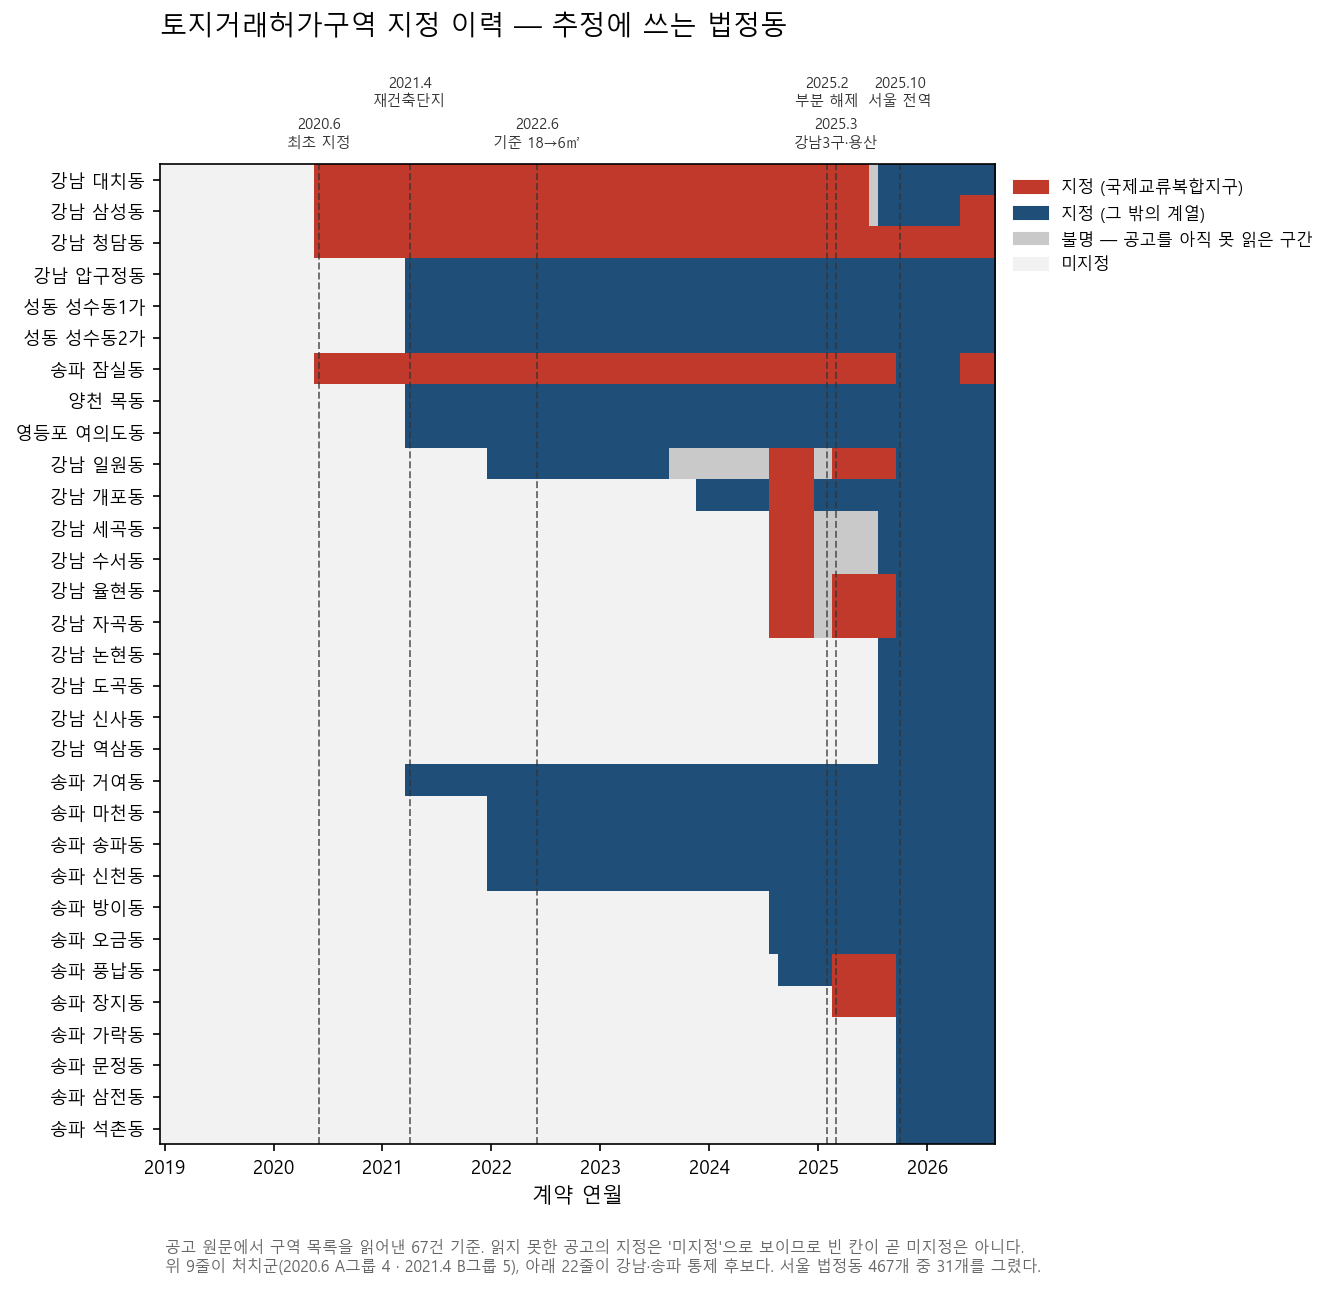
\includegraphics[width=\linewidth]{ltz_heatmap_report.png}
  \caption[토지거래허가구역 지정 이력 --- 추정에 쓰는 법정동]{%
    토지거래허가구역 지정 이력. 가로축은 계약 연월, 한 행이 한 법정동이다.
    \textbf{위 아홉 줄이 처치군}(2020.6 A그룹 넷 · 2021.4 B그룹 다섯),
    아래가 강남·송파 통제 후보다. 붉은색은 국제교류복합지구 계열 지정으로
    A그룹의 처치가 이 계열이다. 점선 여섯이 2.2절의 사건이며,
    \textbf{2025-10 에서 모든 행이 덮이는 것}이 인과 추정을 2025-10-19 에서
    끊는 이유다(0002). 통제 후보 가운데 2025년 이전에 파랗게 칠해지는 동들이
    9.3절에서 빼는 오염 동이다. 회색은 공고 원문에서 구역 목록을 아직 읽어내지
    못한 구간으로, \textbf{빈 칸이 곧 미지정은 아니다}. 서울 전역 467개 동을
    같은 방식으로 그린 것은 \texttt{output/figures/}에 있다.}
  \label{fig:heatmap}
\end{figure}

\subsection{선행연구 세 편과 재현}

2020년 6월 지정을 다룬 국내 연구 세 편을 확인했다. 셋 모두 2025년에 발표됐고,
셋 모두 \textbf{동 단위 집계 자료}를 쓰며, 셋 모두 처치를 \textbf{2020년 6월 단일
사건}으로 취급한다.

말로 비판하는 대신 \textbf{세 편의 사양을 이 연구의 자료로 직접 돌렸다}
(\texttt{scripts/replicate/}). 세 가지가 나왔다.

\textbf{(가) 전상현 외(2025)} --- 동-월 패널 675개(27개 동 $\times$ 25개월)에
구역더미, 시점더미, 교호항, 거래건수를 넣은 OLS다. 같은 격자를 재현하면 거래가
한 건도 없는 \textbf{빈 셀이 31개}이고 전부 통제동이다. 논문 기술통계의 가격
최솟값이 0인 것으로 보아 그 빈 셀을 0으로 코딩한 것으로 보이며, 그렇게 하면 네
계수와 $R^2$가 모두 논문값에 근사하게 재현된다(교호항 $+0.3549$, 논문
$+0.2928$). 그런데 \textbf{빈 셀을 정상적으로 제외하면 교호항이 $-0.0448$로
부호가 뒤집힌다.} 거래가 없는 달의 ``평균 가격''은 0이 아니라 결측이다.

같은 논문이 \textbf{거래건수를 통제변수로} 넣은 것도 문제다. 거래량 감소는
정책의 결과이므로 통제하면 효과의 일부를 빨아들인다. 빼면 교호항이 $-0.1121$
($p=0.002$), 동·월 고정효과까지 넣으면 $-0.1215$가 된다.

\textbf{(나) 이한웅·이춘원(2025)} --- 잠실동을 처치, 송파구 나머지 동을 통제로
두었다. 본문은 이중차분을 표방하나 \textbf{보고된 $t$-검정은 각 집단 내부의
사전-사후 비교}이며 이중차분 계수가 아니다. 논문 표의 수치로 차이의 차이를 직접
계산하면 $\pm$3개월 $+12.2$\,\%p, $\pm$6개월 $-2.9$\,\%p, $\pm$12개월
$-3.9$\,\%p로 \textbf{$\pm$6개월부터 부호가 바뀐다}. 잠실동 가격이 유의하게
올랐다는 것은 맞지만, 통제동도 함께 그리고 더 많이 올랐다.

\textbf{(다) 양지영·정준호(2025)} --- 합성대조군법을 썼다. 도너 풀 15개 동 가운데
\textbf{압구정동·성수동1가·성수동2가가 2021년 4월 27일 토허구역으로 지정}됐다.
연구기간 2018-06$\sim$2022-05 중 마지막 13개월 동안 도너의 20\%가 처치를 받은
상태였다. 처치받은 단위를 도너 풀에 두면 반사실 경로가 왜곡된다
\citep{abadie2010synthetic}.

\subsection{왜 결론이 갈렸는가 --- 설계 선택의 분해}

세 편은 서로 다른 결론을 냈다. 전상현은 가격에 영향이 없다고, 이한웅은 올랐다고,
양지영은 억제됐다고 적었다. \textbf{이것이 실질적 차이인가 설계 선택의
산물인가}가 이 연구의 네 번째 연구 질문이다.

이를 답하려고 \textbf{사양 곡선}\citep{simonsohn2020specification}을 썼다.
합리적인 설계 선택을 전부 조합해 한 그림에 놓는 방법이다. 축은 이 연구가 실제로
내린 결정에서 왔고, 각 축의 대안은 \textbf{선행연구가 실제로 쓴 것이거나 이
연구가 고치기 전에 쓰던 것}이다. 지어낸 대안이 아니다.

\[
\underbrace{2}_{\text{처치군}} \times \underbrace{4}_{\text{통제군}}
\times \underbrace{3}_{\text{창}} \times \underbrace{2}_{\text{사건정렬}}
\times \underbrace{2}_{\text{빈칸}} \times \underbrace{2}_{\text{척도}}
= 192 \;\text{가지}
\]

192가지 전부에서 거래량 효과가 음수였다(9.5절). 여기서 중요한 것은 그 사실이
아니라 \textbf{무엇이 추정치의 크기를 갈랐는가}다. 축마다 그 축의 값들이 내는
중위 추정치의 최대 차이를 재면 표~\ref{tab:rq4-axes}와 같다.

% 자동 생성 — scripts/build_tables.py. 손으로 고치지 않는다.
% 출처: output/results/05b_spec_curve.json : 축별_영향.거래량
\begin{table}[htbp]
  \centering
  \caption{설계 선택이 추정치를 가르는 폭 (거래량, 지정 직후 3개월). 사건 시점 정렬이 통제군 정의의 17배다.}
  \label{tab:rq4-axes}
  \begin{tabular}{lr}
    \toprule
    \textbf{설계 선택} & \textbf{추정치 폭 (\%p)} \\
    \midrule
    사건정렬 & 39.6 \\
    척도 & 11.4 \\
    처치군 & 6.7 \\
    통제군 & 2.3 \\
    창 & 1.1 \\
    빈칸 & 0.9 \\
    \bottomrule
  \end{tabular}

  \begin{minipage}{\linewidth}\footnotesize
  \textit{주.} 축별로 그 축의 값들이 내는 중위 추정치의 최대 차이. 달력 월 $-40.5\%$ 대 효력일 $-80.1\%$.
  \end{minipage}
\end{table}


\textbf{사건 시점 정렬이 통제군 정의의 17배다.} 구체적으로 달력 월로 자르면
중위 $-40.5\%$, 효력일에 맞추면 $-80.1\%$다. 지정 효력일이 6월 23일인데 달력
월로 묶으면 2020년 6월 한 칸에 지정 전(1$\sim$22일)과 후(23$\sim$30일)가 섞인다.
실제로 강남·송파의 해당 칸 3,343건 중 1,532건(45.8\%)이 지정 전 거래였다.

\textbf{선행연구끼리 결론이 엇갈린 이유는 지역을 어떻게 나눴느냐가 아니라
날짜를 어디에 맞췄느냐에서 왔다.} 통제군 정의는 2.3\,\%p밖에 가르지 않는다.
세 편이 서로 다른 지역 정의를 쓴 것은 결론 차이의 원인이 아니다.

\subsection{차별점}

이 연구와 선행연구 세 편의 차이를 정리하면 다음과 같다.

\begin{table}[htbp]
  \centering
  \caption{선행연구 세 편과의 차이}
  \label{tab:diff}
  \begin{tabular}{lllll}
    \toprule
    \textbf{항목} & \textbf{전상현 외} & \textbf{이한웅·이춘원} &
    \textbf{양지영·정준호} & \textbf{본 연구} \\
    \midrule
    분석 단위 & 동-월 집계 & 동 패널 & 동 패널 & \textbf{거래 단위} \\
    물건 특성 통제 & 없음 & 불명 & 세대수·건축연도 &
      \textbf{면적·층 + 단지 FE} \\
    사건 시점 정렬 & 달력 월 & 달력 & 달력 & \textbf{효력일} \\
    처치 구조 & 2020.6 단일 & 2020.6 단일 & 2020.6 단일 &
      \textbf{2020/2021/2025} \\
    2021.4 지정 & --- & --- & \textbf{미반영(도너 오염)} & 반영 \\
    사전추세 검정 & 없음 & 필요성만 언급 & SCM 사전적합 &
      \textbf{사건연구 + 민감도} \\
    거래량 & \textbf{통제변수로 사용} & 기술통계 & --- & \textbf{주 결과변수} \\
    코드 공개 & --- & --- & --- & \textbf{전 과정} \\
    \bottomrule
  \end{tabular}
\end{table}

가장 뚜렷한 두 지점은 \textbf{처치 역전}과 \textbf{동일 동 내 파급효과}다. 처치
역전 자체는 방법론적으로 확립되어 있고\citep{dechaisemartin2020twoway} 적용
사례도 있다. 이 사례의 특징은 역전 간격이 \textbf{39일}로 극히 짧아 거시 환경과
계절성이 사실상 고정되어 있었다는 점, 그리고 해제가 전면적이 아니라 부분적이어서
\textbf{같은 동 안에 규제 상태가 다른 단지가 공존}한다는 점이다. 뒤쪽이 7장의
조건이 된다.

% 3장 자료와 시스템. CS 기여. 8~10쪽.
% 쓰는 방식: "무엇을 만들었다" 가 아니라 "그게 없었으면 2층이 불가능했다".

\section{자료와 시스템}

제목의 1층이 이 장이다. 다만 \textbf{잘게 쪼갠 것 자체는 기여가 아니다.} 의의는
\textbf{미시 자료가 아니면 보이지 않는 것을 실제로 보였다}는 데 있다. 이 장의
각 절은 그 대응 관계를 밝히는 순서로 쓴다.

\begin{table}[htbp]
  \centering
  \caption{미시 자료가 아니면 보이지 않는 것}
  \label{tab:micro-need}
  \begin{tabular}{p{5.2cm}p{4.0cm}p{5.0cm}}
    \toprule
    \textbf{발견} & \textbf{필요했던 미시 정보} & \textbf{동 단위 집계로는} \\
    \midrule
    직후 효과 $-59\% \to -76\%$ & 거래 하나하나의 \textbf{계약일} &
      달력 월 안에서 지정 전후를 못 가른다 \\
    공고와 효력 사이 나흘의 막차 수요 & 하루 단위 거래 & 안 보인다 \\
    면적 기준이 회피 통로 & 거래마다의 \textbf{전용면적} &
      동 전체 거래 수만 있어 불가능 \\
    중위가가 11포인트 부풀려짐 & \textbf{같은 집}의 반복 거래 &
      구성 변화를 못 걷어낸다 \\
    2025년 부분 해제 & \textbf{단지}별 해제·유지 여부 &
      같은 동 안의 두 집단을 못 가른다 \\
    `인근 급등'이 기준점의 산물 & 서울 전역 단지를 \textbf{한 표}에 &
      처치동 인근만 보게 되어 기준점을 못 옮긴다 \\
    두 사건을 \textbf{같은 자}로 & 서울 25개 구를 하나의 패널로 &
      사건마다 통제군이 달라져 차이를 못 잰다 \\
    \bottomrule
  \end{tabular}
\end{table}

선행연구가 동 단위 집계로 ``60\% 줄었다''에서 멈춘 이유가 여기 있다. 그 이상으로
나아갈 정보가 자료에 없었다.

\subsection{실거래 상세 자료}

국토교통부가 공개하는 아파트 매매 실거래 자료는 두 종류다. 일반 자료와
\textbf{상세 자료}(\texttt{RTMSDataSvcAptTradeDev})이며 활용신청이 개별적으로
필요하다. 상세 자료라야 \texttt{aptSeq}(단지 식별자), \texttt{excluUseAr}
(전용면적), \texttt{floor}(층), \texttt{buildYear}(건축연도), 그리고 계약
\textbf{일자}가 함께 온다.

정제를 마친 표본은 표 \ref{tab:sample}과 같다. \textbf{같은 자료를 두 장으로
짓는다} --- 분석 8개 자치구와 서울 25개 자치구다. 뒤쪽이 필요한 이유는 통제군에
있다. 합성대조군은 처치동과 비슷한 동을 서울 전역에서 찾아야 하고(9.2절),
2021년 B그룹은 영등포·양천·성동구까지 걸쳐 있어 8개 구 안에 통제군이 없다
(9.6절). \textbf{기준점을 옮겨 가며 파급을 재는 것}도 서울 전역 패널이라야
가능하다(7.3절).

% 자동 생성 — scripts/build_tables.py. 손으로 고치지 않는다.
% 출처: output/results/02_build.json
\begin{table}[htbp]
  \centering
  \caption{표본 요약. 두 장을 함께 짓는 이유는 \textbf{통제군}에 있다 --- 합성대조군의 기증자 풀과 2021년 B그룹 분석이 서울 전역 패널을 쓴다.}
  \label{tab:sample}
  \begin{tabular}{lrr}
    \toprule
    \textbf{} & \textbf{분석 8개 자치구} & \textbf{서울 25개 자치구} \\
    \midrule
    거래 (건) & 472,782 & 1,407,186 \\
    단지 (aptSeq) & 3,502 & 9,240 \\
    법정동 & 108 & 343 \\
    자치구 & 8 & 25 \\
    반복매매 쌍 & 377,289 & 1,158,318 \\
    제외 --- 취소거래 & 6,293 & 17,307 \\
    제외 --- 신고지연 절단 & 3,156 & 13,677 \\
    계약일 구간 & 2006-01-02 \textasciitilde{} 2026-05-31 & 2006-01-01 \textasciitilde{} 2026-05-31 \\
    수집 시점 & 2026-09-03 & 2026-09-03 \\
    \bottomrule
  \end{tabular}

  \begin{minipage}{\linewidth}\footnotesize
  \textit{주.} 같은 스냅샷에서 같은 규칙으로 정제했다. 분석 패널은 8개 자치구(강남·서초·송파·강동·성동·광진·동작·용산), 서울 패널은 25개 자치구 전체다. 반복매매 쌍은 (단지, 전용면적, 층) 조합의 재거래이며 보유 180일 미만을 뺀 수다(0018).
  \end{minipage}
\end{table}


단지 식별자가 왜 결정적인지는 간단한 예로 알 수 있다. 어느 동에서 한 달에
100건이 팔리다가 20건으로 줄었다고 하자. 줄어드는 비율이 단지마다 다르면
\textbf{각 단지의 가격이 하나도 변하지 않아도 동 평균은 움직인다.} 측정된
``평균 가격 변화'' 안에 진짜 가격 변화와 구성 변화가 섞인다. 실제로 처치동
사후 표본의 평균 전용면적이 93.9\,m$^2$에서 88.7\,m$^2$로 이동했다.

사양 12개를 비교해 보면 \textbf{단위 고정효과 수준이 결과 크기를 두 배 갈랐다}
(0003). 법정동 수준에서 비교하면 가격 효과가 $-12.3 \sim -15.8\%$, 단지 수준으로
내리면 $-6.0 \sim -8.0\%$다. 창 길이($\pm$12/24/36개월)와 통제군 범위(2개 구/8개
구)는 거의 영향이 없었다. \textbf{결과를 좌우하는 유일한 설계 선택이 단위
고정효과였다.}

\subsection{공고 원문에서 법정동 패널까지}

토허구역의 ``어디가 언제''는 공고에만 있다. 그래서 공고를 자료로 다룬다.

\begin{enumerate}[leftmargin=2em, itemsep=2pt]
  \item \textbf{원문 수집.} 서울시보와 전자관보에서 지정·재지정·해제 공고를
        모은다. 서울시보 원본은 2.9\,GB라 저장소 밖에 두고, 발췌한 PDF만 넣는다.
  \item \textbf{본문 텍스트 추출.} PDF에서 글자를 뽑되, 글꼴마다 한글 코드가
        다르게 매핑되는 문제를 글꼴별 오프셋으로 교정한다
        (\texttt{lib/pdftext.py}).
  \item \textbf{구역 표 추출.} 공고 별표에서 자치구·법정동·지번·면적 기준을
        읽는다. 판독 건수는 현재 1,168건이다.
  \item \textbf{지정 구간 생성.} 같은 법정동의 공고들을 시간 순으로 이어 붙여
        \texttt{[시작일, 종료일)} 구간으로 만든다.
  \item \textbf{거래에 결합.} 거래의 계약일과 법정동으로 그 시점의 규제 상태를
        붙인다.
\end{enumerate}

여기서 두 가지 판단이 필요했다.

\textbf{(가) 지정 범위를 동 전체로 볼 것인가}(0010). 공고는 지번 단위로 적는
경우와 동 전체로 적는 경우가 섞여 있다. 2020년 6월 공고는 네 개 동을 동 전체로
지정했음을 지형도면으로 확인했다. 확인 과정에서 외부 자료가 효력일을
2020-06-19로 답했으나 \textbf{공고 2020-1832호 원문은 2020-06-23}이었다. 원문을
따랐다. 2차 자료의 한계를 보여 주는 사례다.

\textbf{(나) 유지 단지를 어떻게 확정할 것인가}(0008). 2025년 2월 부분 해제에서
지정이 유지된 단지를 단지명으로 맞추면 자료마다 14개, 13개, 15개로 갈렸다.
공고 제2025-497호 별표의 \textbf{지번}으로 매칭해 실거래 자료의
\textbf{16개 단지 식별자}로 확정했다(선경이 1차·2차로, 한보미도맨션이 1·2로
나뉜다).

\textbf{(다) 통제군 오염 점검}(0009, 0020). 통제군에 있어야 할 동이 나중에
토허구역으로 지정되면 처치·통제 격차가 줄어 추정치가 0 쪽으로 끌린다. 강남·송파
통제동 23개 가운데 여섯(거여·압구정·마천·송파·신천·일원)이 분석 창 안에서
지정됐음을 찾았고, \textbf{제외 목록을 결과를 보기 전(2026-09-07)에 확정}한 뒤
분석했다(9.3절).

\subsection{표본 정제}

정제 규칙은 둘이다(0004).

\textbf{취소거래 제외.} \texttt{cdealType}이 \texttt{'O'}인 해제 거래를 뺀다.
8개 자치구·2026-09-03 수집 기준 원자료 482,231건 중 6,293건(1.30\%)이다. 신고 후
취소되는 거래에는 시세 조작 목적의 허위 신고가 섞일 수 있고, 규제 시점 전후로
몰리면 추정치를 위로 편향시킨다.

\textbf{신고지연 절단.} 신고기한이 계약일로부터 30일이라 수집 시점에 가까운
계약월은 신고가 덜 들어와 과소집계된다. 2026-05에서 06으로 넘어가며 거래가 절반
이하로 떨어지므로 보수적으로 \textbf{2026-05까지만} 쓴다. 신고율을 추정해
역산하는 방법도 있으나 그 추정의 불확실성을 자료에 섞어 넣게 되므로 버리는 쪽을
택했다.

이 연구에는 \textbf{절단이 둘}이고 섞이기 쉬우므로 분명히 둔다. 자료 품질 때문에
표본 끝을 2026-05-31에서 끊고(0004), 통제군 소멸 때문에 인과추정을
2025-10-19에서 끊는다(0002). \textbf{뒤쪽이 더 강한 제약}이므로 신고지연 절단은
실제로 인과추정에 영향을 주지 않는다.

\textbf{뺀 것이 결과를 바꾸는지 확인했다}(0030). 취소거래를 다시 넣어 같은 사양을
돌리면 지정 직후 효과가 $-79.8\%$에서 $-79.5\%$로 \textbf{0.3\,\%p} 움직인다.
규제 직후에 몰리지도 않는다 --- 세 사건에 대해 취소율의 이중차분이 창에 따라
$-2.3 \sim +1.7$\,\%p로 부호가 바뀐다(9.7절).

\subsection{자체 가격지수}

거래가 80\% 줄면 팔리는 물건의 구성이 바뀌므로, 가격을 해석하려면 구성 변화를
걷어내야 한다. 약점이 \textbf{정반대}인 두 방법을 모두 지었다.

\textbf{반복매매지수}(0018)는 같은 물건의 두 거래만 쓴다. 같은 집이면 면적·층·
단지·입지가 전부 같으므로 구성이 원천적으로 바뀔 수 없다. 추정식은
\[
\log P_{t_2} - \log P_{t_1} = \beta_{t_2} - \beta_{t_1} + \varepsilon
\]
이고, $t_2$에 $+1$ · $t_1$에 $-1$인 희소 행렬로 회귀한다
\citep{bailey1963regression}. 오래 보유한 쌍일수록 가격 변화의 분산이 커지므로
\citet{caseshiller1987}의 3단계 가중을 쓴다 --- 잔차 제곱을 보유기간에 회귀하고
그 역수의 제곱근으로 다시 추정한다. 실측 기울기가 보유 1년당 분산 $+0.006$으로
가정과 맞았다.

세 가지를 정했다. 첫째, 실거래 자료에 \textbf{호실 번호가 없으므로} 물건을
(단지, 전용면적, 층)으로 본다. 월 단위로 5.8\%의 칸에 두 건 이상이 들어가지만,
같은 단지·면적·층이면 가격이 거의 같아 서로 바뀌어 짝지어져도 편의가 2차적이다.
둘째, \textbf{보유 180일 미만을 뺀다} --- `가격 변화가 정확히 0'인 쌍의 비중이
4.1\%에서 1.5\%로 떨어지고 그 뒤로는 완만하다. 셋째, 연율 로그수익률 $\pm$50\%
초과를 뺀다(전체의 0.5\%).

\textbf{헤도닉 지수}(0025)는 반대로 모든 거래를 쓰되 특성을 통제한다.
\[
\log(\text{㎡당가}) \sim \text{월 더미} + \log(\text{면적}) +
\log(\text{면적})^2 + \text{층 구간 더미}
\]
월 더미가 지수다. \textbf{연식은 넣지 않는다} --- 단지 고정효과 아래에서 연식은
시간의 일차함수라 월 더미에 완전히 흡수된다(제거 후 잔차 $10^{-10}$). 넣어도
계수는 같지만 읽는 사람이 통제된 줄로 오해한다.

% 자동 생성 — scripts/build_tables.py. 손으로 고치지 않는다.
% 출처: output/results/08_hedonic.json : 지수_사다리
\begin{table}[htbp]
  \centering
  \caption{구성 통제의 사다리. 아래로 갈수록 더 많은 것을 고정한다.}
  \label{tab:index-ladder}
  \begin{tabular}{lrrr}
    \toprule
    \textbf{가격지수} & \textbf{지정 전 비} & \textbf{지정 후 비} & \textbf{변화 (\%)} \\
    \midrule
    중위가(총액) & 0.945 & 0.849 & -10.1 \\
    중위가(㎡당) & 1.012 & 0.885 & -12.5 \\
    헤도닉 & 0.979 & 0.870 & -11.1 \\
    헤도닉+단지 & 0.985 & 0.927 & -5.9 \\
    반복매매 & 1.001 & 0.941 & -6.0 \\
    \bottomrule
  \end{tabular}

  \begin{minipage}{\linewidth}\footnotesize
  \textit{주.} 약점이 정반대인 두 방법(헤도닉과 반복매매)이 $-5.9\%$ 와 $-6.0\%$ 에서 만난다. 집계 지수의 $-10 \sim -12\%$ 는 절반쯤이 구성 변화였다.
  \end{minipage}
\end{table}


\begin{figure}[htbp]
  \centering
  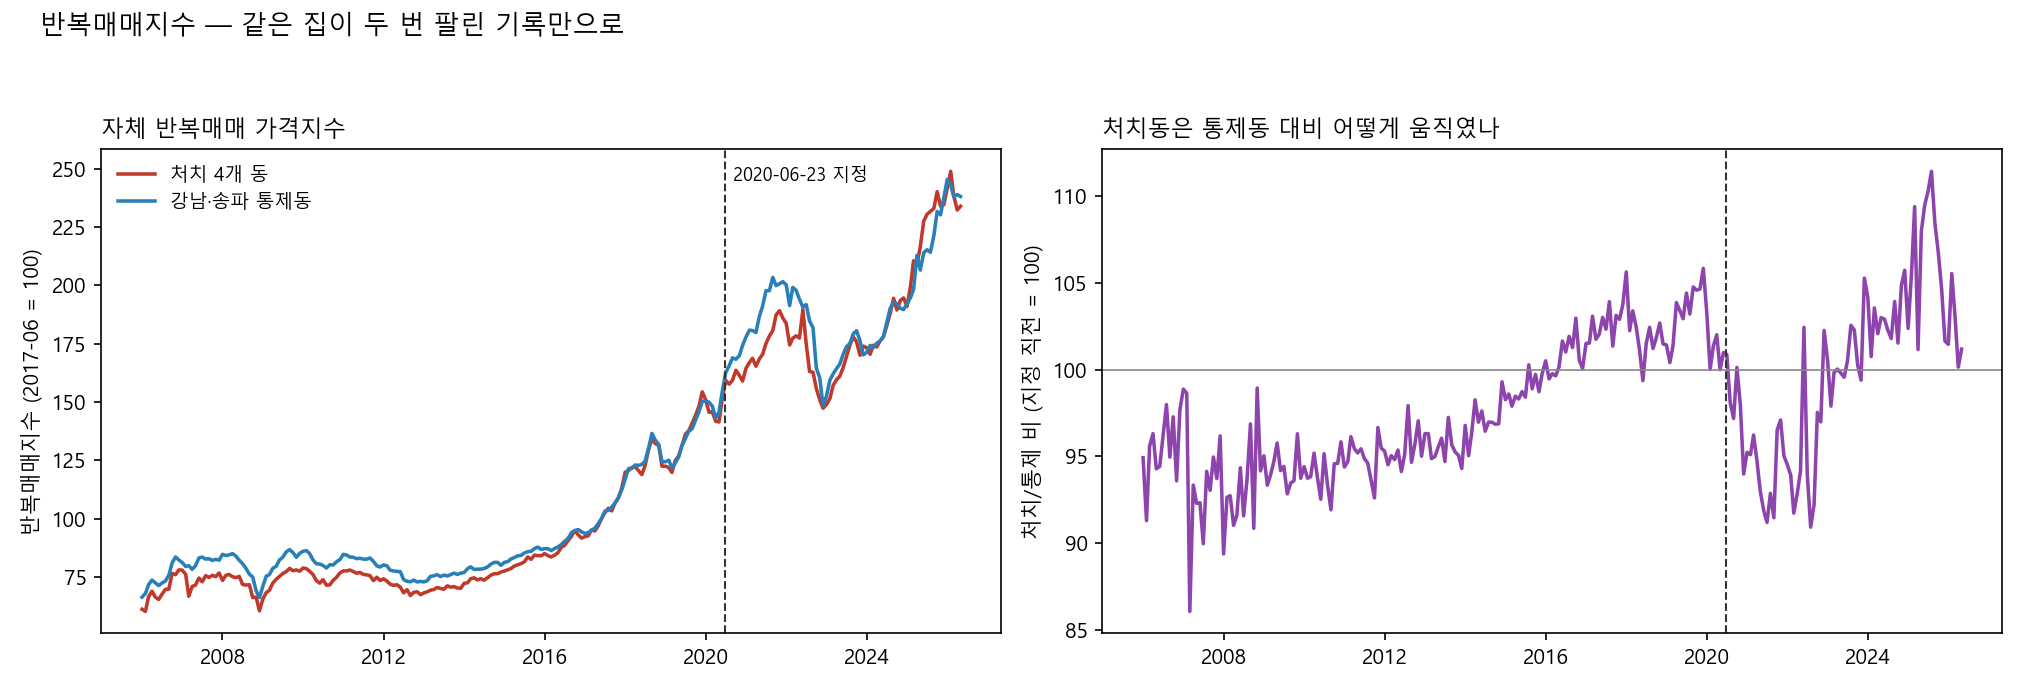
\includegraphics[width=\linewidth]{07_repeat_sales.png}
  \caption{반복매매 가격지수. 2017-06 = 100.}
  \label{fig:repeat-sales}
\end{figure}

\textbf{약점이 정반대인 두 방법이 $-5.9\%$와 $-6.0\%$에서 만난다.} 반복매매는 두
번 팔린 집만 쓰고(선택편의), 헤도닉은 관측되는 특성만 통제한다. 둘이 일치하면
서로를 떠받친다. 그리고 집계 지수의 $-10 \sim -12\%$는 \textbf{절반쯤이 구성
변화}였음을 보여 준다.

지수 자체의 그럴듯함도 확인했다. 2017-06을 100으로 두면 2021-06에 187,
2022-06에 190, 2023-06에 169($-11\%$), 2026-05에 237이다. 2022년 금리 급등기의
조정과 이후 재상승이 그대로 나타난다.

\subsection{재현 장치}

\textbf{이 절이 이 보고서에서 가장 `시스템'다운 부분이다.} 숫자가 아니라
\textbf{숫자를 믿게 만드는 장치}를 지었다는 이야기다.

원자료 수집부터 그림·표 생성까지 \textbf{\pipeSteps 단계 파이프라인} 하나로 돈다
(\texttt{python run\_all.py}). 단계는 자료 \pipeData, 정책 \pipePolicy, 분석
\pipeAnalysis, 재현 \pipeReplicate, 시각화 \pipeViz, 문서 \pipeDocs 로 나뉘고,
뒤 단계가 앞 단계 산출물을 읽으므로 하나라도 실패하면 거기서 멈춘다. 그림
\ref{fig:pipeline}이 전체 흐름이다.

\textbf{이 문단의 단계 수도 손으로 적지 않았다.} 주차 보고서가 한 편 늘면 문서
단계가 하나 늘기 때문에, 손으로 적으면 그 순간 틀린 값이 된다. 도식을 그리는
스크립트가 \texttt{run\_all.py}의 단계 표를 읽어 세고 그 값을 매크로로 내보낸다.

\begin{figure}[htbp]
  \centering
  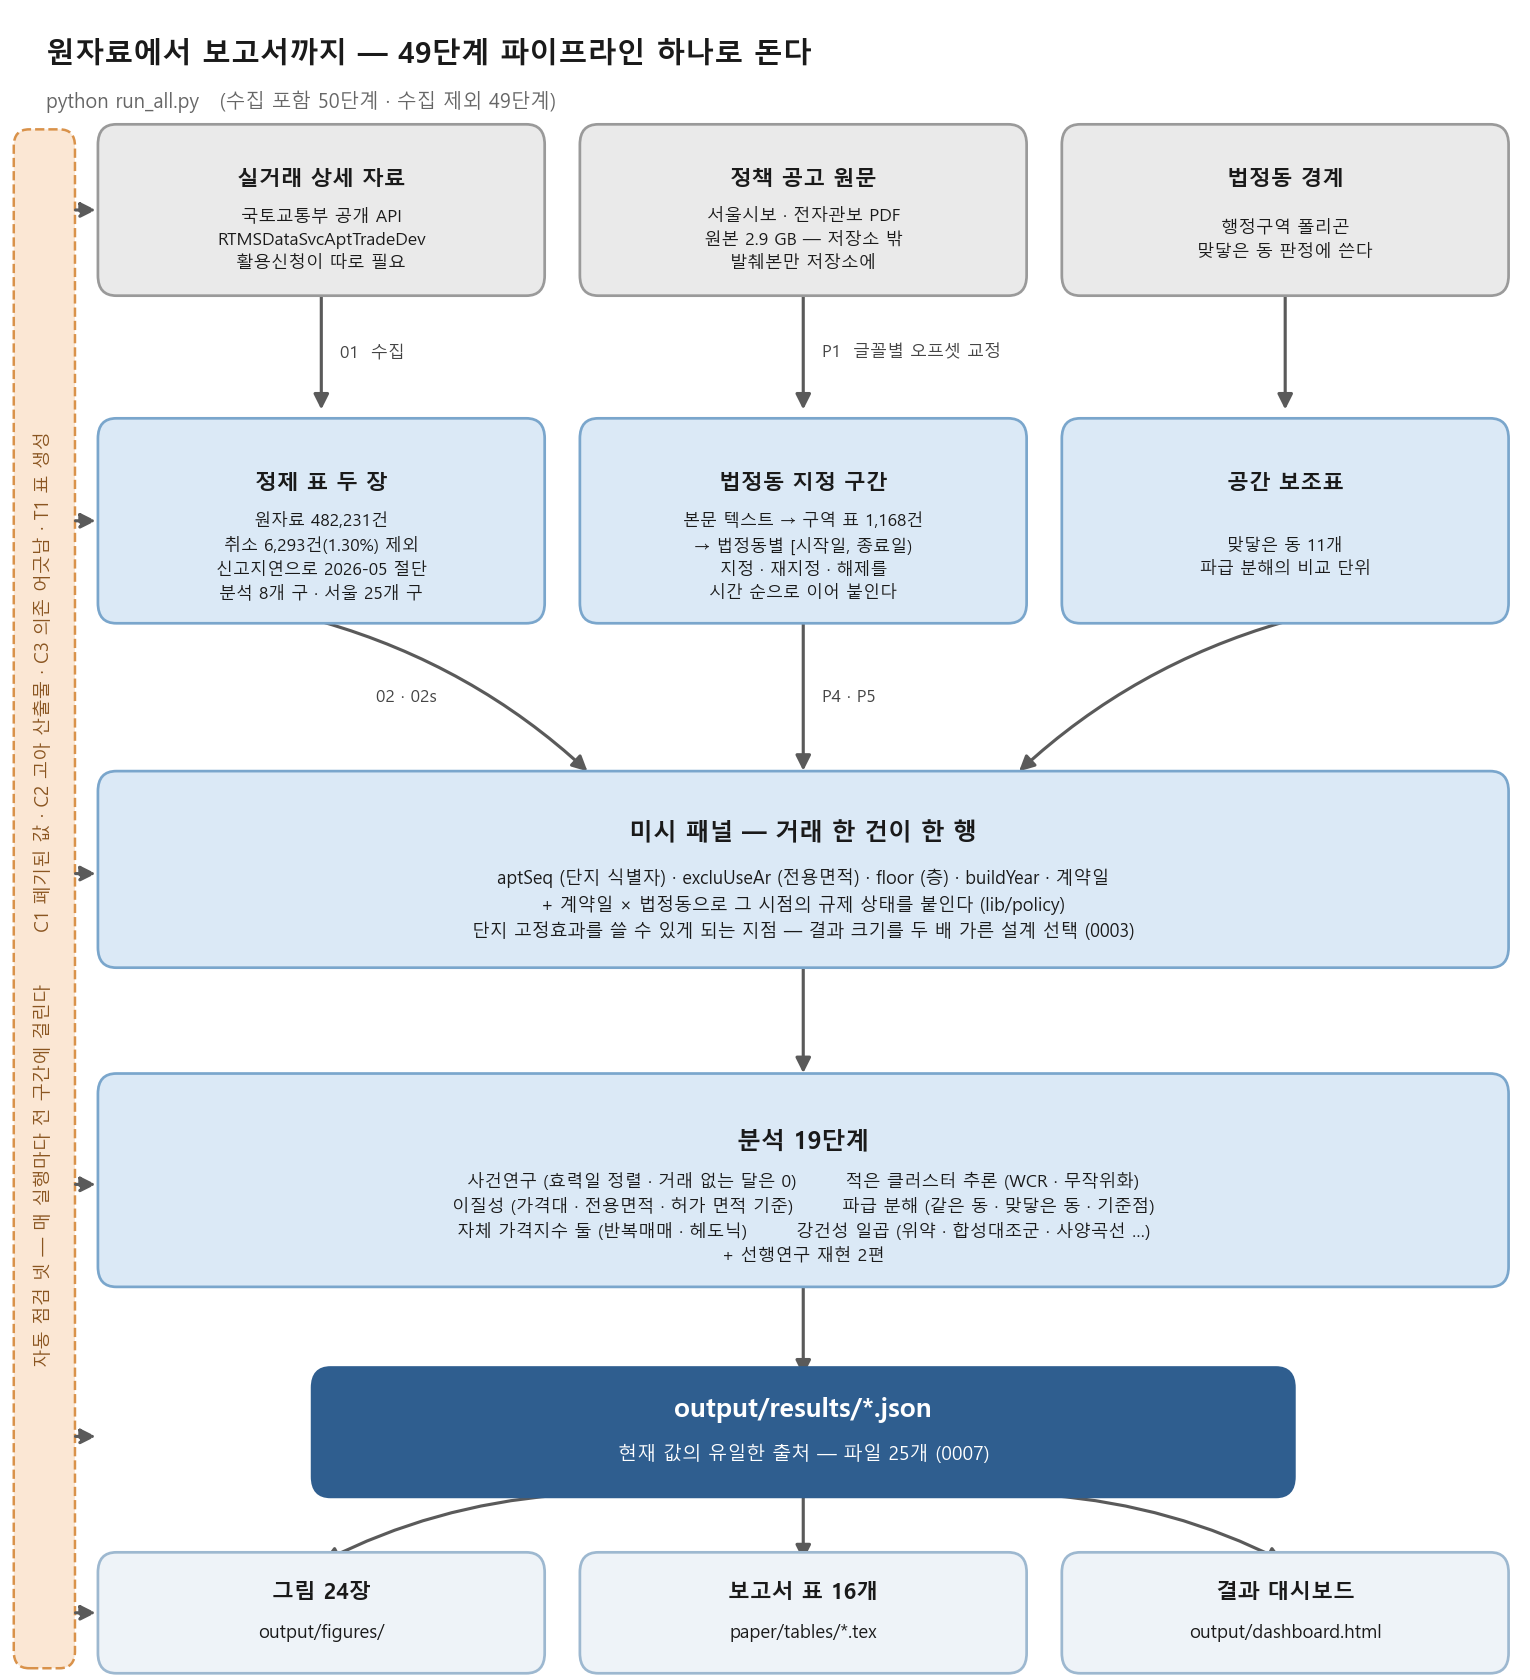
\includegraphics[height=0.86\textheight]{pipeline.png}
  \caption[원자료에서 보고서까지 --- \pipeSteps 단계 파이프라인]{%
    원자료에서 보고서까지. 입구는 셋이지만 \textbf{출구는 하나}다 ---
    현재 값의 출처는 \texttt{output/results/*.json} 하나이며(0007), 보고서의 표와
    결과 대시보드는 거기서 생성된다. 가운데 줄기(공고 PDF $\to$ 법정동 지정
    구간)가 없으면 처치 변수 자체가 없다. 왼쪽 띠의 점검 넷은 분석 뒤가 아니라
    매 실행마다 걸린다. \textbf{이 그림의 숫자도 손으로 적은 것이 아니라
    \texttt{run\_all.py}와 산출물 폴더를 센 것이다.}}
  \label{fig:pipeline}
\end{figure}

그 위에 점검 넷이 매 실행마다 걸린다.

\begin{table}[htbp]
  \centering
  \caption{자동 점검 넷}
  \label{tab:checks}
  \begin{tabular}{llp{7.5cm}}
    \toprule
    \textbf{단계} & \textbf{스크립트} & \textbf{무엇을 잡나} \\
    \midrule
    C1 & \texttt{check\_numbers.py} &
      살아있는 문서와 결정기록에 남은 \textbf{폐기된 값}.
      조건이 붙은 줄은 통과시킨다 \\
    C2 & \texttt{check\_stale.py} &
      이번 실행에서 \textbf{다시 만들어지지 않은} 산출물,
      그리고 만들어 놓고 \textbf{아무도 가리키지 않는} 문서 \\
    C3 & \texttt{check\_deps.py} &
      \texttt{requirements.txt}와 실제 import의 어긋남.
      함수 안의 늦은 import까지 AST로 훑는다 \\
    T1 & \texttt{build\_tables.py} &
      보고서의 표를 결과 JSON에서 생성. 가리키는 키가 없으면 알린다 \\
    \bottomrule
  \end{tabular}
\end{table}

설계 원칙은 하나다. \textbf{현재 값의 출처는 \texttt{output/results/*.json}
하나다}(0007). 문서의 숫자가 이 파일과 어긋나면 JSON이 맞다. 그래서 보고서의
표와 결과 대시보드는 \textbf{숫자를 손으로 적지 않는다} --- 적는 것은 ``어디서
꺼낼지''와 ``어떻게 보일지''뿐이다.

문서는 세 종류로 나눈다. \textbf{동결}(주차 보고서·발표 자료)은 그 시점의
기록이므로 갱신하지 않고, \textbf{살아있는}(백로그·용어집·연구의 뼈대)은 항상
현재 상태이며, \textbf{최종}(이 보고서)은 하나의 조건으로 통일한다. 다만 동결
문서라도 \textbf{작성 시점에 이미 틀린 값}은 정정하고 그 사실을 남긴다.

\subsection{클린 환경 재현}

장치가 돈다는 말을 하려면 \textbf{받는 사람의 환경}에서 확인해야 한다. 새 폴더에
내려받아 새 가상환경에서 돌렸다.

\textbf{멈췄다.} 12단계에서 \texttt{shapely}를 찾지 못했다.
\texttt{requirements.txt}에 \texttt{shapely}와 \texttt{markdown}이 빠져
있었던 것이다. 법정동 경계로 맞닿은 동을 찾을 때와 보고서 HTML을 만들 때 쓰는데,
작업 환경에는 다른 경로로 깔려 있어 몇 주 동안 드러나지 않았다.
\textbf{받는 사람만 겪고 만드는 사람은 못 보는 고장}이다.

고친 뒤 전 단계가 돌았고(약 21분) \textbf{\texttt{output/results/*.json} 25개가
바이트 단위로 같았다.} 그리고 같은 일이 다시 생기지 않도록 \texttt{check\_deps.py}를
만들어 파이프라인에 넣었다.

절차에서 알게 된 것 셋을 \texttt{README}에 적었다. 첫째, \textbf{원자료는
재수집하면 안 된다} --- 실거래 자료는 취소와 지연신고로 소급 갱신되므로 다시
받으면 다른 자료가 온다. 재현은 \textbf{같은 스냅샷 위에서} 하는 것이다. 둘째,
윈도의 경로 길이 한계(260자) 때문에 깊은 폴더에서는 \texttt{statsmodels} 설치가
깨진다. 셋째, 그림을 매번 커밋해 \texttt{.git}이 936\,MB다.

\subsection{유령 숫자 사건}

앞 절의 장치들을 \emph{왜} 만들었는지가 이 절이다.

\texttt{output/results/es\_price.csv}와 \texttt{es\_volume.csv}가 2026-09-03
파일이었다. 그 사이 사건연구 스크립트가 JSON 저장으로 바뀌면서
\textbf{아무도 그 CSV를 만들지 않게 됐다.} 그래서 사건 시점 정렬 수정(0013)
\emph{이전} 숫자($k=0$에서 $-58.7\%$)가 석 달 가까이 남아 있었다.

\textbf{전체 재실행을 두 번 했는데도 못 잡았다.} 전체 재실행은 다시 만들어지는
파일만 본다. 아무도 만들지 않는 파일은 \texttt{git status}에도 뜨지 않고 영원히
낡은 채로 남는다.

그래서 \texttt{check\_stale.py}를 만들었다. 바뀐 것이 아니라 \textbf{안 바뀐
것}을 센다. 붙이자마자 다섯을 더 잡았다. 고아 파일 네 개를 지웠고, 그중
\texttt{current\_zones.csv}에는 유지 단지가 ``14개''로 적혀 있었다 --- 0008에서
16개로 확정한 뒤 폐기된 숫자다. 그리고 결정기록 0004에 \textbf{6개 자치구 시절
값}(4,285건)이 남아 있었다. 결정기록이 검사 대상에서 빠져 있었기 때문에 다섯 달
동안 드러나지 않았다. 검사 대상에 넣은 뒤 \textbf{나머지는 전부 깨끗했다}
(당시 28편, 현재 30편).

\textbf{제목의 두 층이 여기서 만난다.} 1층(미시 패널 구축)은 2층(인과추정)이
답할 수 있게 해 주는 전제이고, 그 전제가 썩지 않게 지키는 것이 이 절의 장치들이다.
제안서가 ``데이터 엔지니어링이 분석의 부속물이 아니라 식별 전략의 전제''라고 쓴
것이 이 뜻이며, 6장의 면적 기준 발견이 그 주장의 가장 좋은 증거다.

% 4장 식별 전략. 0001 · 0011 · 0012 · 0013 · 0003 · 0014 · 0002 · 0022

\section{식별 전략}

\subsection{왜 거래량인가}

당초 계획은 가격을 주 결과변수로 두는 것이었다. 선행연구 세 편이 모두 가격을
다루므로 비교가 쉽기 때문이다. \textbf{자료를 보고 바꿨다}(0001).

\textbf{첫째, 이론적으로 옳다.} 토허제는 가격 상한제가 아니라 거래에 허가라는
마찰을 부과하는 제도이므로 1차 반응이 나타나는 지점은 거래량이다. 가격은 거래량이
줄어든 뒤에 오는 2차 반응이다.

\textbf{둘째, 가격은 사전 추세를 넘지 못한다.} 2020년 6월 사건에서 가격의 사전
계수가 $k=-5, -4, -3$에서 각각 $+0.026$, $+0.032$, $+0.034$로 모두 유의하며
\textbf{한 방향으로 매끈하게} 움직인다. 기준 분기로 올수록 격차가 줄어들고
있었다는 뜻이고, 그 하강을 연장하면 사후의 하락과 구별되지 않는다.

\textbf{셋째, 거래량이 60\% 감소하면 거래 물건의 구성이 변한다.} 가격 해석에
앞서 거래량 반응을 규명해야 하는 순서상의 이유가 있다(3.1절).

여기서 흔한 오해 하나를 미리 정리한다. \textbf{거래량도 사전 추세를 위배한다}
(0014). 다만 위배의 \emph{모양}이 다르다. 가격은 한 방향으로 누적되고, 거래량은
인접한 두 분기가 반대로 흔들린다. 가격과 갈리는 지점은 \textbf{위배의 유무가
아니라 그 위배가 추정치를 위협하는지}다(4.5절).

이 판단은 다섯 달 뒤 세 가지 방법으로 확인됐다 --- 사양 곡선(192/192 대 144 중
70), 사전추세 민감도 구간(붕괴값 1.62 대 0.22), 합성대조군($p=0.007$ 대 0.511).
가격은 버리지 않고 \textbf{선행연구와의 대조 지점}으로 8장에 둔다.

\subsection{처치군과 통제군}

\textbf{처치군}은 2020년 6월 23일 동 전체가 지정된 네 개 법정동(대치·삼성·청담·
잠실)이다(0012). 2021년 4월 지정(B그룹)은 9.6절에서 별도 사건으로 다룬다.

\textbf{통제군}은 \textbf{같은 구(강남·송파) 안의 비지정 동}이다(0011). 바깥 구가
아니라 같은 구 안으로 둔 이유는 학군·교통·생활권과 거시 충격이 가장 가깝기
때문이다. 강남·송파 비처치동 23개 가운데 분석 창 안에 지정된 여섯을 뺀 사양을
반드시 함께 보고한다(9.3절).

통제군 선정에서 확인한 사실 하나. 처치군 거래의 \textbf{63.9\%}가 시가 15억원
초과이고 통제 자치구는 0.3$\sim$3.9\%다. 같은 서울 안에서 노출도가 20배 차이난다.
이것이 6장의 출발점이 된다.

\subsection{사건 시점 정렬}

\textbf{이 절의 선택 하나가 추정치를 39.6\,\%p 가른다}(2.4절).

지정 효력일은 2020년 6월 23일이다. 거래를 달력 월로 묶으면 ``2020년 6월'' 한 칸에
지정 전(1$\sim$22일)과 후(23$\sim$30일)가 섞인다. 실제로 그 칸 3,343건 중
1,532건(45.8\%)이 지정 전 거래였다. 그래서 \textbf{효력일에 맞춘 월}을 쓴다 ---
한 달이 23일에 시작해 다음 달 22일에 끝난다(0013).

\[
k(\text{거래일}) = \left\lfloor \frac{\text{효력일 기준 경과 개월}}{3} \right\rfloor,
\qquad k=0 \;\text{은 효력일 직후 3개월}
\]

\textbf{거래가 한 건도 없는 달을 0으로 채운다.} \texttt{groupby}에서 빠진 채로
두면 `거래가 있었던 달'만 보게 되어 감소 효과가 과소추정된다. 법정동 27개 $\times$
사건월 51개 = 1,377칸 가운데 90칸이 0이다.

두 선택을 함께 적용해 직후 효과가 $-59\%$에서 $-76\%$로 바뀌었다. 선행연구의
``60\%''는 \textbf{달력 월로 센 값}이다.

\subsection{단지 고정효과}

기본 사양은 \textbf{단지 $\times$ 계약월 양방향 고정효과}이고 면적과 층을 추가로
통제한다(0003). 가격 회귀는 거래 단위, 거래량 회귀는 법정동 $\times$ 사건월
패널이다. 거래 건수는 거래 하나에서 정의되지 않으므로 거래량만큼은 집계가
불가피하다.

\[
\log(\text{건수}_{dt}) = \sum_{k \neq -1} \beta_k \cdot
(\text{처치}_d \times \mathbb{1}[k_t = k]) + \alpha_d + \gamma_t + \varepsilon_{dt}
\]

$\alpha_d$는 법정동, $\gamma_t$는 사건월 고정효과다. 0이 있으므로
$\log(1+n)$을 쓴다. 표준오차는 법정동으로 군집한다.

$\beta_k$가 뜻하는 것은 \textbf{$k$분기의 처치-통제 격차에서 기준 분기의 격차를
뺀 값}이다. 격차의 차이이므로 수준의 차이는 고정효과가 이미 걷어 간다.

\subsection{평행추세와 사전 추세 위배}

사건 시점을 효력일에 맞추고 사전 구간을 제대로 출력하니 \textbf{거래량도 사전
추세를 위배했다.} $k=-2$가 $-48.0\%$($p<0.001$), $k=-3$이 $-24.4\%$($p=0.046$)다.

처음에는 \textbf{12·16 대책}(2019-12-16, 시가 15억 초과 주담대 전면 금지)을
의심했다. $k=-2$가 그 직후 창이고 처치군의 15억 초과 거래 비율이 63.9\%이기
때문이다. \textbf{의심이 틀렸다.} 월 단위로 펴 보니 사전 기간의 격차가 기준월
대비 \emph{내내} 음수였다. 추세가 기울어진 것이 아니라 \textbf{기준월 하나가
높았다.}

\begin{itemize}[leftmargin=2em, itemsep=1pt]
  \item $k=-1$ (기준, 2020-03-23$\sim$06-22): 격차 $+1.334$
  \item 사전 24개월 평균: $+0.857$ (표준편차 0.232)
  \item 차이: $+0.477$ --- \textbf{2$\sigma$ 밖}
  \item 12·16 이전 평균 $+0.909$ 대 이후 평균 $+0.670$, 차이 $-0.239$
\end{itemize}

\textbf{기준월 이상치($+0.477$)가 12·16 효과($-0.239$)의 두 배다.} $k=-1$은
코로나 1차 유행이 잦아들며 거래가 반등하고 6·17 대책과 지정을 앞둔 막차 수요가
겹친 분기이며, 바로 앞 $k=-2$는 12·16 직후라 반대로 눌려 있다.

세 가지로 다시 쟀다.

\textbf{(가) 기준 분기를 바꾼다.}

% 자동 생성 — scripts/build_tables.py. 손으로 고치지 않는다.
% 출처: output/results/06d_pretrend.json : A_기준분기
\begin{table}[htbp]
  \centering
  \caption{기준 분기를 옮겨 본 거래량 효과. $k=-2$ 만 크게 튄다.}
  \label{tab:pretrend-ref}
  \begin{tabular}{lrrrr}
    \toprule
    \textbf{기준 분기} & \textbf{$k{=}0$} & \textbf{$k{=}1$} & \textbf{$k{=}4$} & \textbf{사전 유의 칸} \\
    \midrule
    -1 & -79.8 & -66.8 & -39.7 & 3 \\
    -2 & -61.2 & -36.2 & 16.0 & 6 \\
    -3 & -73.3 & -56.2 & -20.3 & 3 \\
    -4 & -77.8 & -63.4 & -33.5 & 2 \\
    -5 & -78.4 & -64.5 & -35.5 & 2 \\
    -6 & -78.6 & -64.8 & -36.0 & 1 \\
    \bottomrule
  \end{tabular}

  \begin{minipage}{\linewidth}\footnotesize
  \textit{주.} $k=-2$ 는 12·16 대책 직후라 눌려 있는 분기다. 나머지는 $-73 \sim -80\%$ 로 좁게 모인다.
  \end{minipage}
\end{table}


\textbf{$k=-2$를 기준으로 쓸 때만 크게 튄다.} 나머지는 $-73 \sim -80\%$로 좁게
모이고, 기준을 멀리 둘수록 사전 유의 개수가 3에서 1로 줄어든다. 위배가 추세가
아니라 인접 분기의 흔들림임을 가리킨다.

\textbf{(나) 사전 구간을 자른다.} 12·16 대책을 사전에서 빼든 넣든 $k=0$이
$-74.2\%$, $-73.8\%$, $-73.3\%$로 거의 같다. 처음의 의심이 여기서 명확히
기각된다.

\textbf{(다) 사전 기울기를 사후로 늘려 뺀다.} 사전 계수에 직선을 맞추면 기울기가
분기당 $-0.0334$이고(기준 분기의 고정된 0을 포함하면 $-0.0003$으로 거의 0이다 ---
불리한 쪽을 썼다), 보정하면 $k=0$이 $-69.0\%$로 버티지만 사후 후반은 무너진다.

\begin{figure}[htbp]
  \centering
  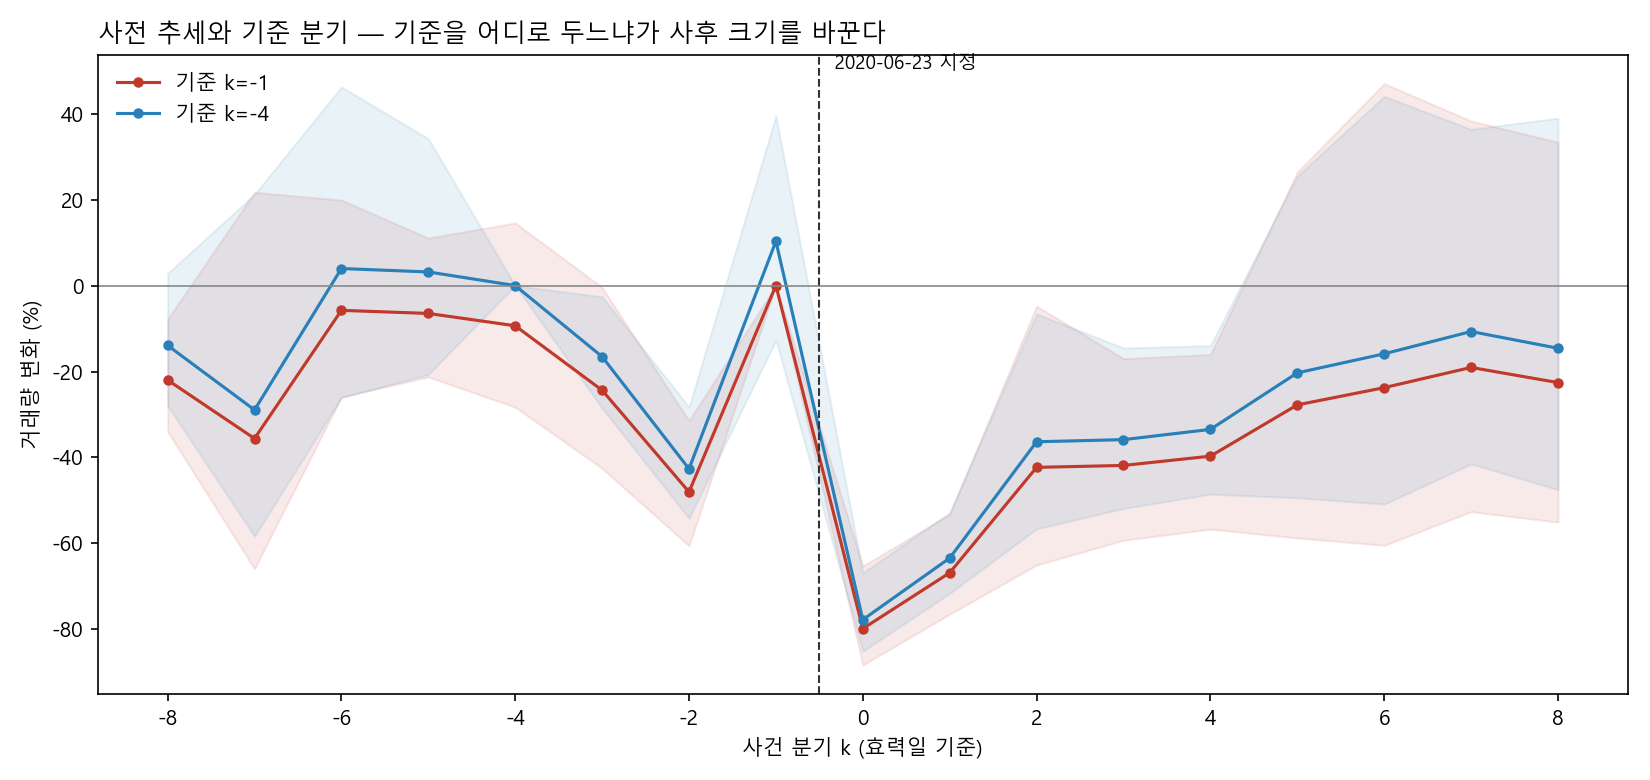
\includegraphics[width=\linewidth]{06d_pretrend.png}
  \caption{사전 추세 진단. 기준월 하나가 높았고 인접 두 분기가 반대로 흔들린다.}
  \label{fig:pretrend}
\end{figure}

\textbf{결정은 셋이다}(0014). 주 사양은 관행대로 $k=-1$을 유지한다. 지정 직후
효과는 \textbf{구간으로} 보고한다($-74 \sim -80\%$, 합성대조군까지 넣으면
$-71 \sim -80\%$). 그리고 \textbf{사후 $k \geq 4$는 해석하지 않는다} --- 기준
선택에 $-20 \sim +16\%$로 흔들리고 기울기 보정에도 부호가 뒤집힌다. ``효과가
얼마나 오래 갔는가''는 이 설계로 답할 수 없다.

\subsection{분석 구간}

인과추정 대상 기간을 \textbf{2025-10-19까지}로 한정한다(0002). 10·15 대책으로
2025-10-20부터 토허구역이 서울 25개 자치구 전체로 확대되어 \textbf{서울 안에
미처치 아파트가 존재하지 않는다.} 나흘 앞선 10-16에 규제지역도 서울 전역으로
확대되어 두 정책의 효과 분리도 불가능하다.

경기 미지정 지역을 통제군으로 쓰는 대안은 시장 구조가 달라 평행추세 방어가
어렵고, 경기 12개 지역도 동시에 지정되었다. \textbf{이 제약은 한계가 아니라 설계
근거다} --- 정책 타임라인을 읽고 식별 가능 구간을 스스로 잘라낸 판단이다.

\subsection{사전 등록한 예측}

6장에서 효과의 이질성이 허가 대상의 면적 기준에서 왔다는 결론에 이른다. 그
결론이 맞다면 \textbf{다른 자료에서 특정한 결과가 나와야 한다.} 그 예측을
결과를 보기 전에 적어 두었다(0022, 2026-09-18).

\begin{quote}
2025년 재지정은 허가 면적 기준이 6\,m$^2$이므로 소형 면제가 거의 없다.
면적 기준이 이질성의 원인이라면 \textbf{2025년에는 소형도 함께 줄어야 한다.}
\end{quote}

대출 가설이 맞았다면 2025년에도 소형은 줄지 않았어야 한다. 두 가설이 반대 방향을
예측하는 지점이다. 답은 6.8절에 있다.

% 5장 주 결과. 0013 · 0014 · 0019 · 0017

\section{주 결과 --- 얼마나 줄었나}

\subsection{지정 직후 거래량}

2020년 6월 23일 지정 직후 3개월 거래량은 \textbf{반사실 대비 $-71 \sim -80\%$}다.
단일 숫자가 아니라 구간으로 적는 이유는 둘이다. 기준 분기를 $-1$, $-3$, $-4$,
$-5$, $-6$ 중 어디에 두어도 $-73 \sim -80\%$ 안에 들어가고(4.5절), 합성대조군이라는
전혀 다른 방법으로 재면 $-71.0\%$다(9.2절).

\textbf{모든 수치는 반사실 대비임을 다시 밝힌다}(0006). ``거래가 80\% 줄었다''가
아니라 ``지정이 없었을 때보다 80\% 적다''는 뜻이다. 통제동도 같은 기간에 줄었고,
그만큼을 뺀 나머지가 여기 적힌 값이다.

\subsection{사건연구 궤적}

한 숫자로 요약하기 전에 분기별 궤적을 먼저 본다. 사전 구간이 평평한지, 효과가
언제 시작해 어떻게 줄어드는지가 여기서 드러난다.

\begin{figure}[htbp]
  \centering
  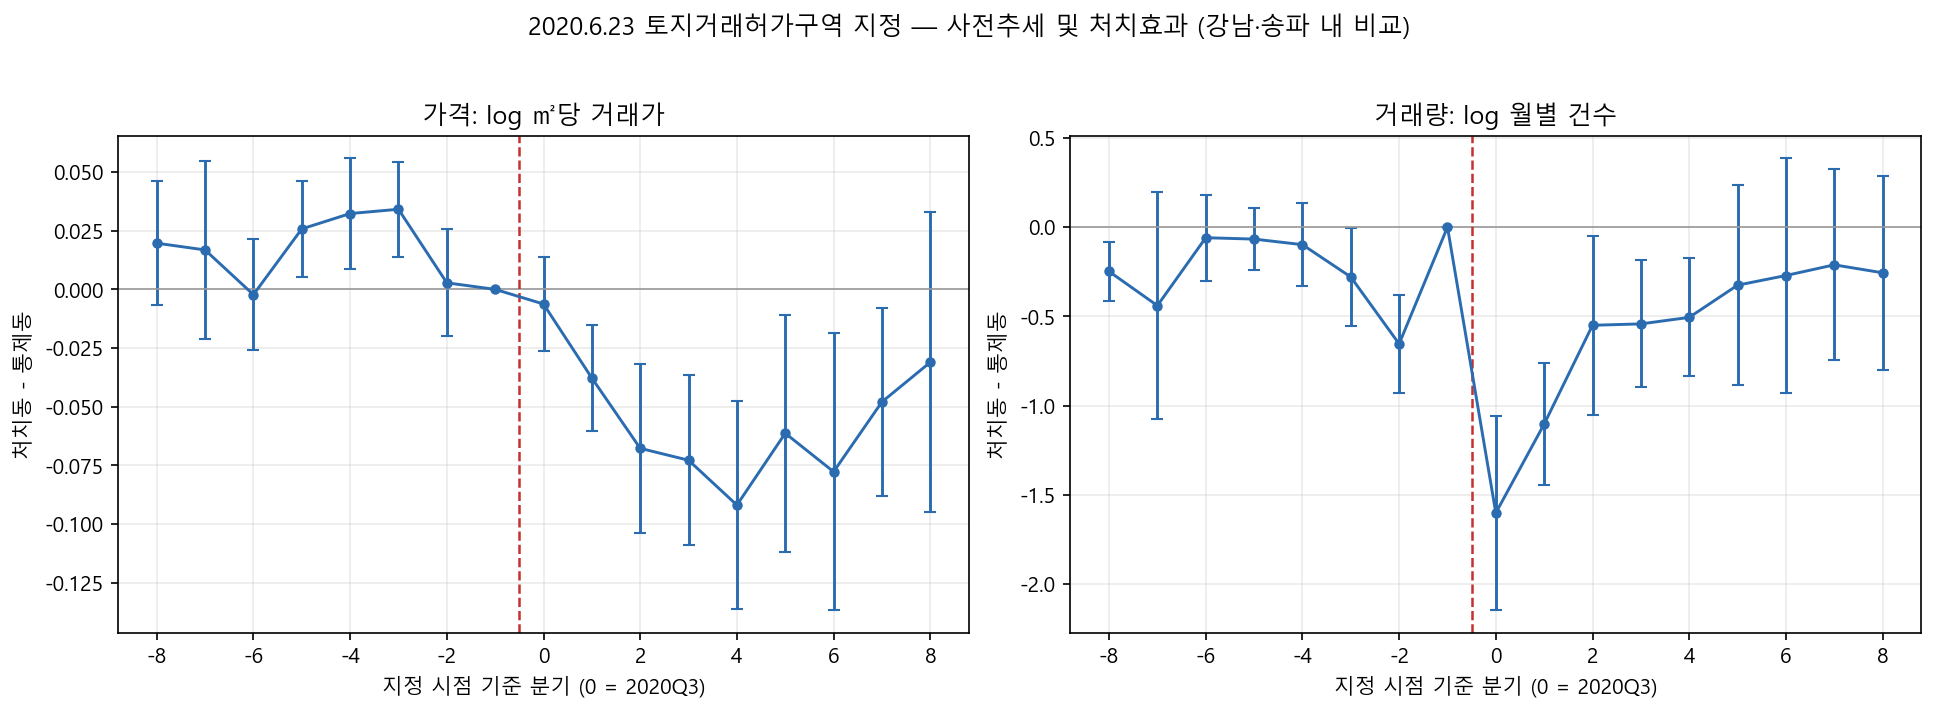
\includegraphics[width=\linewidth]{event_study_2020.png}
  \caption{2020-06-23 지정 사건연구. 왼쪽 가격(log ㎡당가), 오른쪽 거래량
           (log 월별 건수). 세로 점선이 지정 시점, 가로 0선이 기준 분기와
           같다는 뜻이다.}
  \label{fig:event-study-2020}
\end{figure}

그림~\ref{fig:event-study-2020}의 오른쪽이 거래량이다. 지정 분기($k=0$)의 계수가
$-1.6015$이므로 $\exp(-1.6015)-1 = -79.8\%$다. 이후 $k=1$에서 $-66.8\%$,
$k=2$에서 $-42.3\%$, $k=4$에서 $-39.7\%$로 완만해진다.

왼쪽 가격과 대조하면 \textbf{두 결과변수의 모양이 다르다}는 것이 한눈에 보인다.
가격은 사전 구간의 점들이 0 위에 줄줄이 떠 있고 사후에 서서히 내려가며, 거래량은
사전에 0 근처에 모여 있다가 효력일 직후에 수직으로 떨어진다. \textbf{제도가
거래에 마찰을 붙이는 제도라는 사실이 그림에 그대로 나타난다.}

\subsection{적은 클러스터 추론}

처치가 네 개 동뿐이다. 관행적인 군집 표준오차는 묶음이 충분히 많다는 가정 위에
있으므로 \textbf{클러스터가 적으면 표준오차를 작게 잡아 $p$를 과하게 작게
만든다}\citep{mackinnon2017wild}. 실제로 사건연구 $k=0$의 관행 $p$가
$8 \times 10^{-9}$로 나왔다. 그 자체가 증상이다.

두 가지로 다시 쟀다(0019).

\textbf{와일드 클러스터 제약 부트스트랩(WCR).} 귀무가설을 부과한 잔차에 법정동마다
같은 가중을 곱해 가짜 자료를 9,999벌 만들고 $t$ 통계량의 분포를 직접 만든다.
클러스터가 적을 때 권장되는 Webb 6점 분포를 쓴다\citep{webb2014reworking}.

\textbf{무작위화 추론.} 27개 동 가운데 4개를 처치로 고르는 \textbf{모든 경우}
$\binom{27}{4} = 17{,}550$가지를 돌려 진짜 배정이 몇 번째인지 센다
\citep{fisher1935design}. 분포 가정이 전혀 없다.

% 자동 생성 — scripts/build_tables.py. 손으로 고치지 않는다.
% 출처: output/results/06_inference.json
\begin{table}[htbp]
  \centering
  \caption{적은 클러스터 추론. 관행 $p$ 를 버리고 둘을 함께 적는다.}
  \label{tab:inference}
  \begin{tabular}{lrrrr}
    \toprule
    \textbf{사양} & \textbf{효과 (\%)} & \textbf{관행 $p$} & \textbf{WCR $p$} & \textbf{무작위화 순위} \\
    \midrule
    사건연구 k=0 & -79.8 & $<0.001$ & 0.014 & 1 / 17,550 \\
    24개월 이중차분 & -33.5 & 0.016 & 0.050 & 97 / 17,550 \\
    삼중차분 (차이) & -56.1 & 0.002 & 0.027 & 321 / 17,220 \\
    \bottomrule
  \end{tabular}

  \begin{minipage}{\linewidth}\footnotesize
  \textit{주.} 법정동 27개 중 처치가 4개다. WCR 은 Webb 6점 9,999벌, 무작위화는 4개를 고르는 17,550가지 전수.
  \end{minipage}
\end{table}


\begin{figure}[htbp]
  \centering
  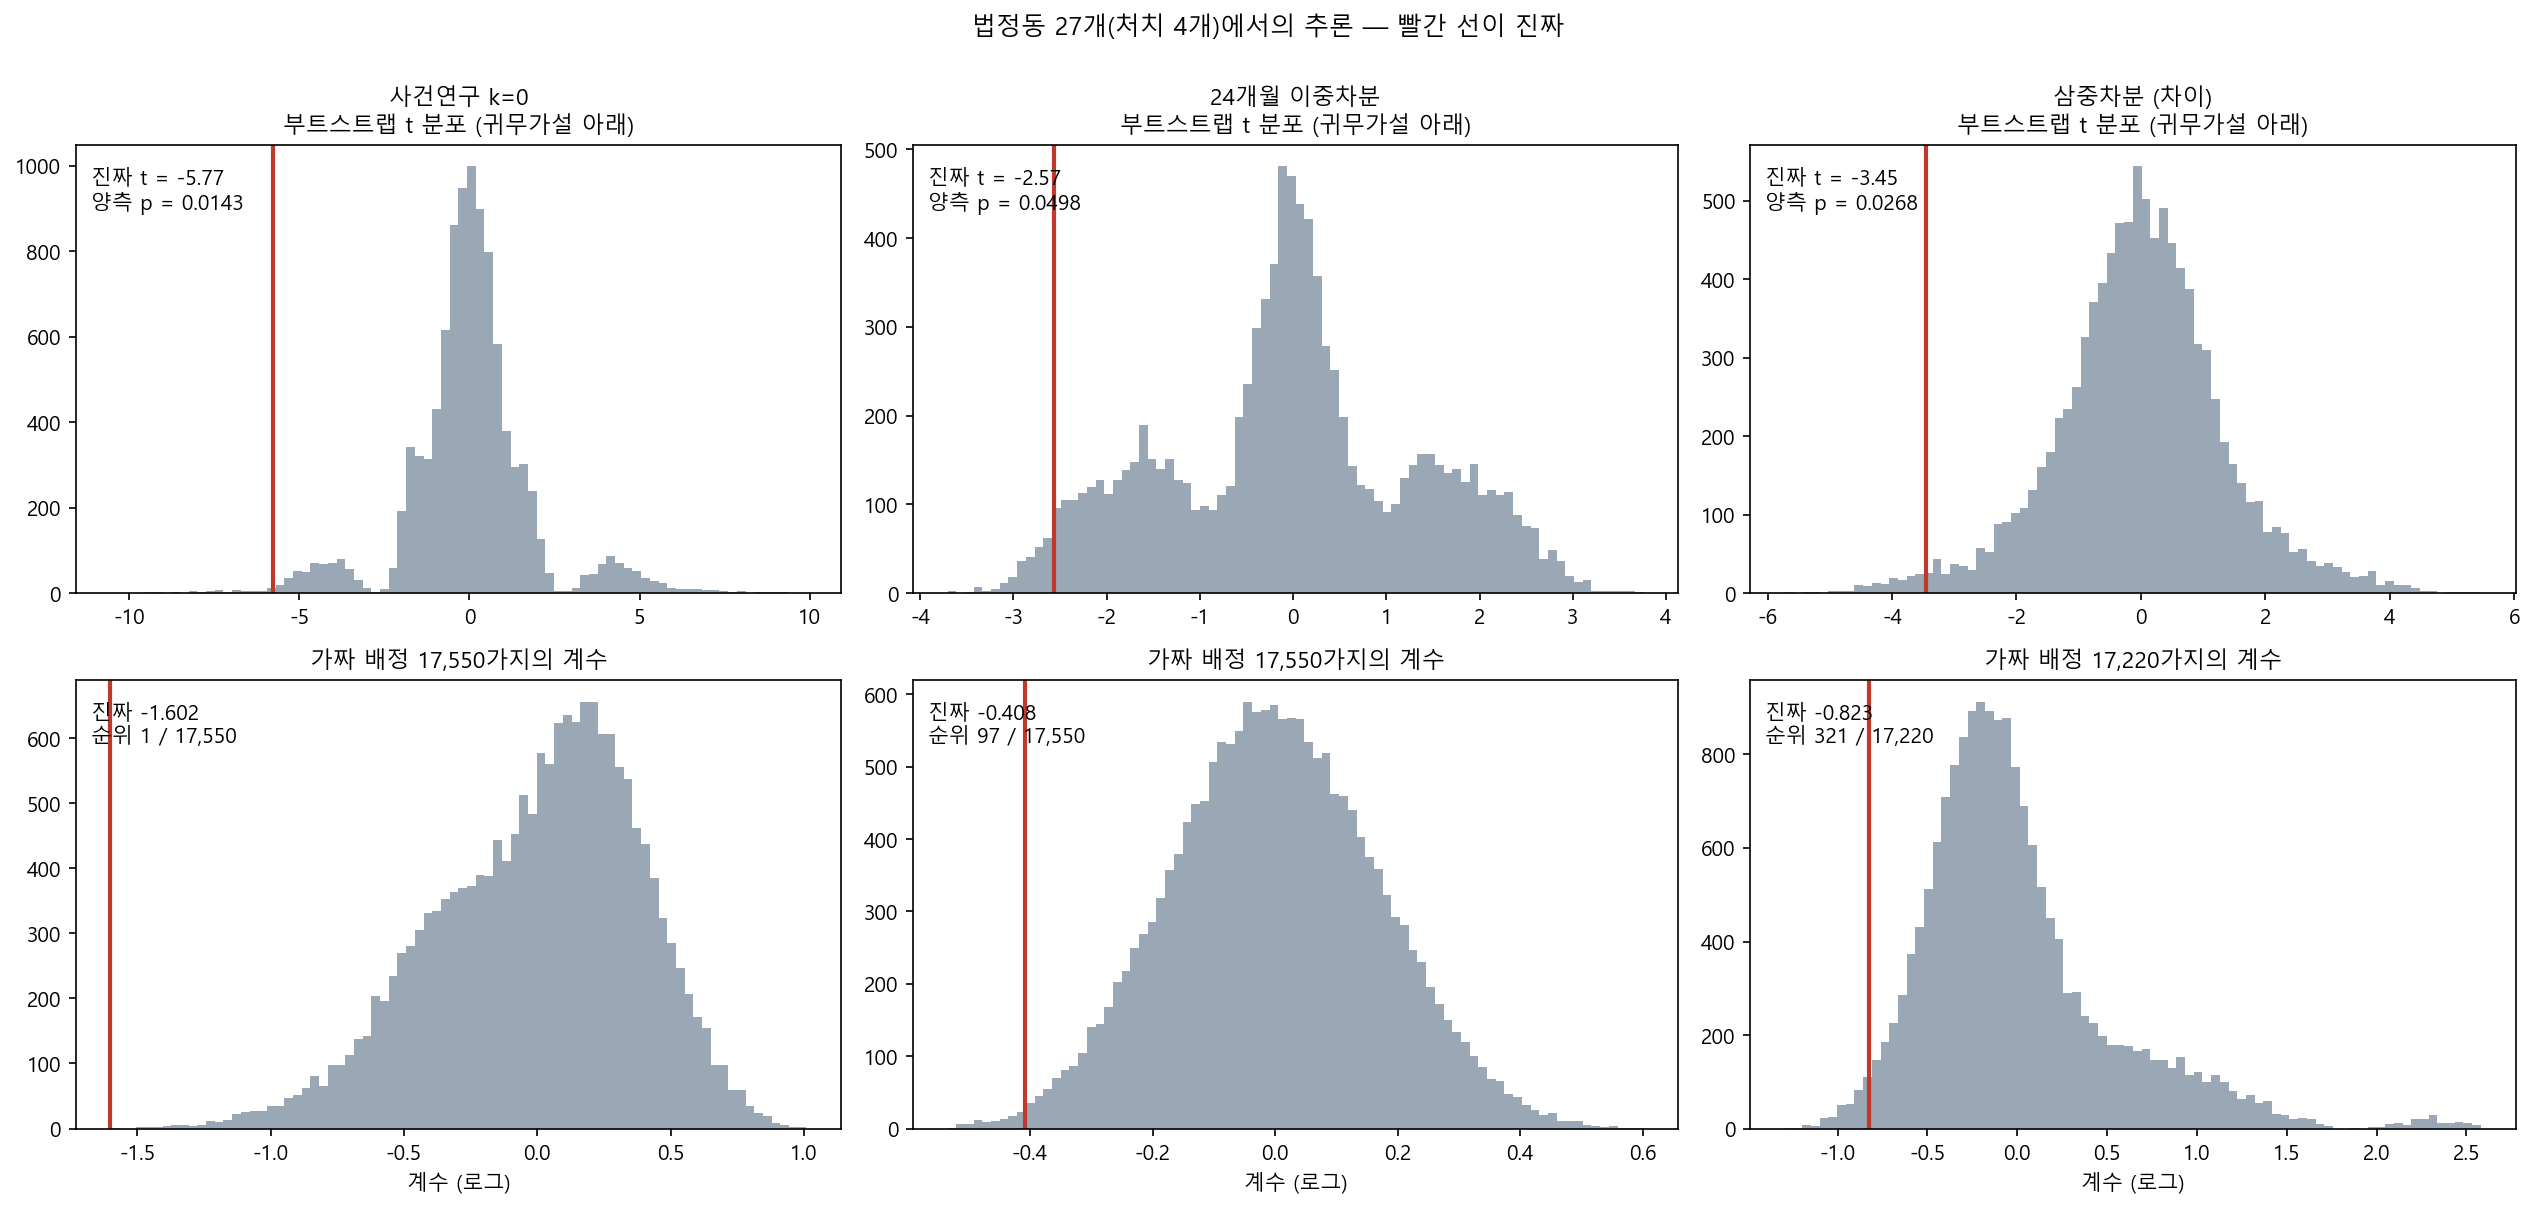
\includegraphics[width=\linewidth]{06_inference.png}
  \caption{와일드 클러스터 부트스트랩과 무작위화 분포. 세로선이 진짜 배정이다.}
  \label{fig:inference}
\end{figure}

\textbf{지정 직후 효과는 어떤 추론으로도 살아남는다.} 17,550가지 배정 중
\textbf{1위}다. 서울 강남·송파의 어느 네 개 동을 골라도 진짜 처치동만큼 지정 직후에
거래가 줄어든 조합은 없다. 관행 $p$ $8\times10^{-9}$는 과장이었지만 결론은 그대로다.

\textbf{다만 ``1위''라는 말은 지정 직후에 한정된다.} 24개월 평균은 97위다.
이 구별을 지키지 않으면 과장이 된다.

\subsection{24개월은 경계에 있다}

사후 24개월을 하나로 묶은 이중차분은 $-33.5\%$이고 WCR $p$가 0.047로
\textbf{0.05에 붙어 있다}. 통제군 오염 동 여섯을 빼면 $-38.4\%$로 커지고 $p$가
0.015로 내려온다(9.3절) --- 경계의 일부는 오염에 의한 감쇠였다.

그러나 \textbf{사전 추세를 모수로 열면 이 값은 버티지 못한다.} 24개월 평균의
붕괴값이 0.05다(8.4절의 방법과 같다). 사전에 관측된 위배의 5\%만 사후에 이어져도
구간이 0을 품는다.

\textbf{그래서 이 보고서는 지속 기간을 말하지 않는다.} 4.5절에서 ``사후
$k \geq 4$는 해석하지 않는다''고 정한 것, 9.2절의 합성대조군에서 사후 27개월
평균이 152개 중 22위($p=0.145$)인 것, 그리고 여기의 붕괴값 0.05가 모두 같은
방향을 가리킨다. \textbf{일시 충격인지 지속적 동결인지는 이 설계로 답할 수 없다.}

% 6장 누구에게 달랐나. 이 연구의 뼈대. 0015 · 0019 · 0021 · 0022 · 0023 · 0029
% 이야기 순서로 쓴다 — 서술이 세 번 바뀐 과정을 숨기지 않는다.

\section{누구에게 달랐나}

이 장은 \textbf{결론만 적지 않고 결론에 이른 순서대로} 쓴다. 서술이 세 번 바뀌었고,
바뀐 과정 자체가 이 연구에서 가장 값어치 있는 부분이기 때문이다.

\begin{table}[htbp]
  \centering
  \caption{이질성 서술이 바뀐 과정}
  \label{tab:het-history}
  \begin{tabular}{llp{7.0cm}}
    \toprule
    \textbf{시점} & \textbf{서술} & \textbf{근거} \\
    \midrule
    1주차 & 15억 이하에서 효과가 더 컸다 & 표본을 갈라 따로 추정 \\
    2주차 & 고가 단지에 집중된다 & 삼중차분 ($p=0.0006$) \\
    3주차 & 방향은 맞으나 단단하지 않다 & 적은 클러스터 추론 \\
    3주차 & \textbf{가격이 아니라 면적 기준일 수 있다} &
      경계 민감도 + 면적대 탐색 \\
    3주차 & \textbf{면적 기준이 주된 원인이다} &
      2022 강화 + 2021 위약 \\
    \bottomrule
  \end{tabular}
\end{table}

\textbf{주 결과(지정 직후 $-71 \sim -80\%$)는 한 번도 움직이지 않았다.} 흔들린
것은 이질성의 해석이다.

\subsection{1주차 질문 --- 대출을 고려해야 하지 않나}

1차 발표에서 지도교수가 ``대출 규제를 고려해야 하는 것 아니냐''고 물었다. 근거
없는 지적이 아니었다. 처치군 거래의 \textbf{63.9\%}가 시가 15억원 초과이고 통제
자치구는 0.3$\sim$3.9\%다. 같은 서울 안에서 노출도가 20배 차이난다. 그리고
15억 초과 주담대 금지(2019-12-17)는 토허구역 지정(2020-06-23)보다 \textbf{6개월
앞선다.}

\subsection{대출 규제 25건을 상쇄 10 / 핵심 4 로 가르다}

대출 규제는 토허제와 자료의 성격이 다르다(0015). 토허제는 ``어디가 언제''가
공고에만 있어 공고를 다 모아야 했지만, 대출 규제는 대부분 \textbf{``어디''가
없다} --- 전국 또는 규제지역 일률이다. 그리고 상당수가 금융감독원 행정지도로 나가
관보에 다 남지도 않는다. \textbf{`전수 수집'이라는 접근 자체가 성립하지 않는다.}

그래서 \textbf{증거 등급}을 나눠 2016년 이후 25건을 1차 자료로 확인하고(1차 19건,
시행일 불명 4건), \textbf{처치군과 통제군에 다르게 걸리는가} 하나로 갈랐다.

\begin{table}[htbp]
  \centering
  \caption{대출 규제 25건의 분류}
  \label{tab:loan-class}
  \begin{tabular}{llp{8.0cm}}
    \toprule
    \textbf{분류} & \textbf{건수} & \textbf{뜻} \\
    \midrule
    \textbf{상쇄} & 10 & 서울 전역 동일 적용. 시간 고정효과가 흡수한다 \\
    \textbf{핵심} & 4 & 집값에 걸려 처치군에 집중된다 \\
    나머지 & 11 & 창 밖 · 영향 작음 · 확인 필요 \\
    \bottomrule
  \end{tabular}
\end{table}

\textbf{규제를 다 모을 필요가 없다는 것이 핵심 통찰이다.} 이중차분에서 양쪽에
똑같이 걸리는 규제는 시간 고정효과가 저절로 뺀다. 다르게 걸리는 것만 골라내면 된다.

남는 넷은 2019-12-17 시가 15억 초과 주담대 전면 금지, 2019-12-23 9억 초과분
LTV 40$\to$20\%, 같은 날 9억 초과 차주단위 DSR 40\%, 그리고 2022-12-01 15억 금지
폐지다. \textbf{넷 다 지역이 아니라 집값에 걸린다.}

\textbf{규제가 실제로 물렸는지부터 확인했다.} 문턱 바로 아래와 위($\pm$0.5억)의
거래 수 비를 재면\citep{bestkleven2018} 규제 이전 0.96배, 금지 기간 \textbf{1.60배},
폐지 이후 1.09배다. 분기별로는 금지 직후 2.1배까지 올랐다가 폐지 분기에 0.81로
떨어진다. \textbf{규제가 켜질 때 쏠림이 생기고 꺼지자 사라진다.}

\begin{figure}[htbp]
  \centering
  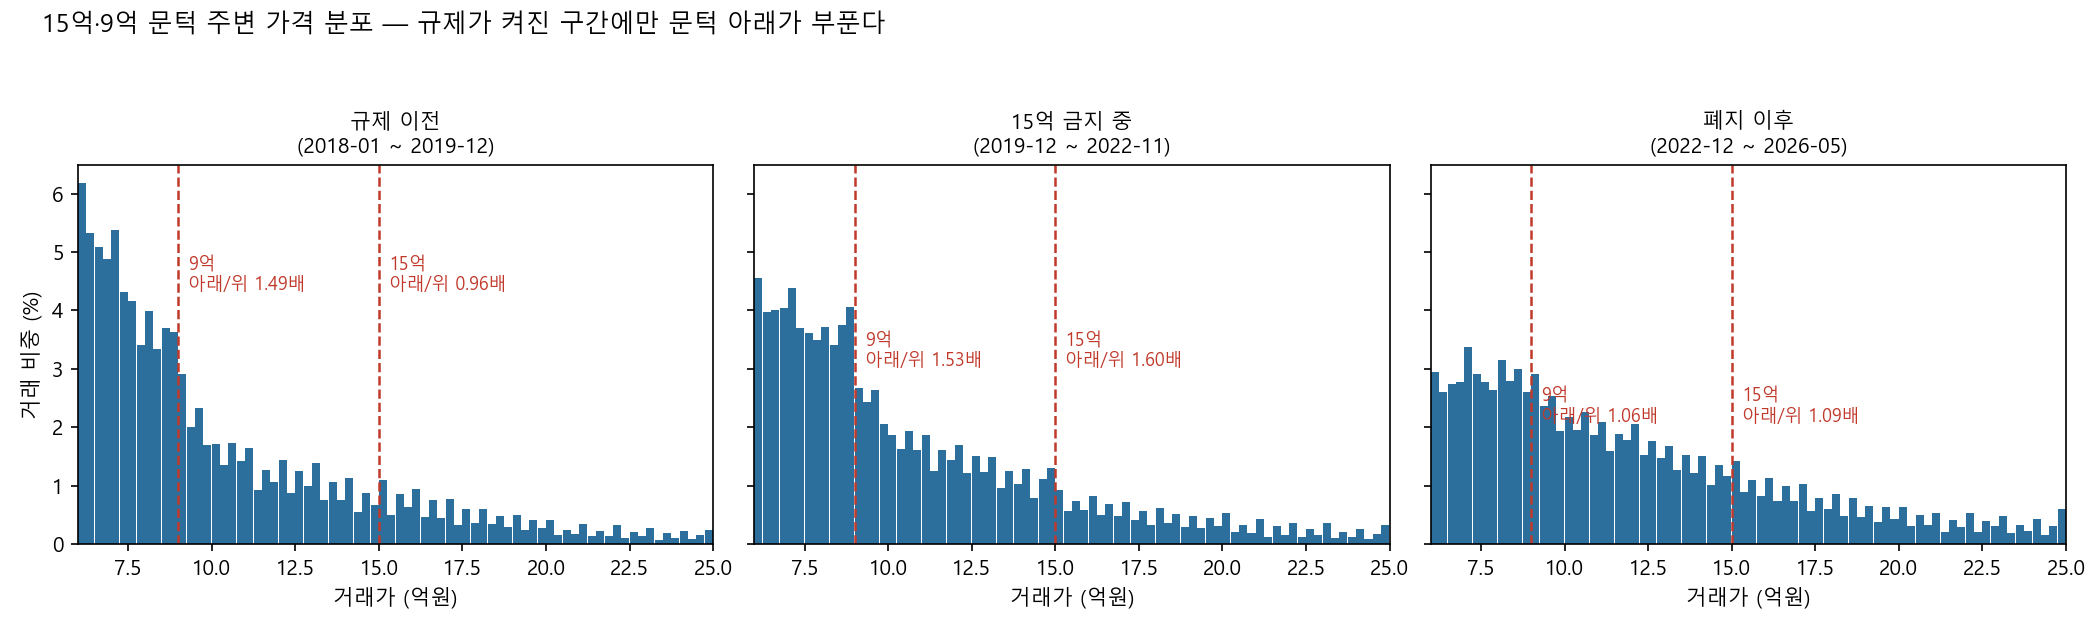
\includegraphics[width=\linewidth]{06c_bunching.png}
  \caption{15억원 문턱의 쏠림. 규제를 따라 켜지고 꺼진다.}
  \label{fig:bunching}
\end{figure}

\textbf{그리고 교란변수가 아님을 셋으로 확인했다.} 첫째, 수준의 불균형은
이중차분에서 문제가 아니다 --- 필요한 것은 추세의 평행이고 수준은 고정효과가
뺀다. 둘째, 상쇄 10건은 시간 고정효과가 먹는다. 셋째, 핵심 4건은 집값에 걸리므로
\textbf{같은 가격대 안에서 비교하면 차분으로 빠진다.} 실제로 고가 통제동이 45\%
줄 때 고가 처치동은 76\% 줄었다. 그리고 12·16 대책을 사전 구간에서 빼든 넣든
$k=0$이 $-73 \sim -74\%$로 바뀌지 않는다(4.5절).

\subsection{삼중차분 --- 고가 단지에 집중된다}

교란이 아니라면 \textbf{이질성 요인}인가. 여기서 두 개념을 구별해야 한다.
교란변수는 처치와 결과에 동시에 영향을 주어 추정치를 \emph{편향}시키고 통제해야
한다. 이질성 요인은 처치 효과의 \emph{크기}를 좌우하므로 \textbf{나눠 봐야 하고
통제하면 안 된다} --- 통제하면 가격 수준 자체를 통제하게 되어 효과의 일부를
빨아들인다(나쁜 통제).

처치군 안에서 15억 초과·이하를 갈라 한 식에 교차항으로 넣었다. \textbf{노출도는
처치 이전에 정해진 값이어야 하므로} 거래 시점 가격이 아니라 12·16 시행 직전 2년의
단지별 중위 거래가를 기준가로 삼았다(전체 거래의 94\%에 기준가가 붙는다).

\begin{table}[htbp]
  \centering
  \caption{가격군별 원자료 --- 법정동 $\times$ 사건월 칸의 평균 거래 건수}
  \label{tab:loan-raw}
  \begin{tabular}{llrrr}
    \toprule
    \textbf{가격군} & \textbf{집단} & \textbf{사전} & \textbf{사후} &
    \textbf{변화} \\
    \midrule
    저가 & 처치 & 7.6 & 3.9 & $-48\%$ \\
    저가 & 통제 & 20.2 & 10.8 & $-47\%$ \\
    \textbf{고가} & \textbf{처치} & \textbf{42.2} & \textbf{10.3} &
      $\mathbf{-76\%}$ \\
    고가 & 통제 & 15.7 & 8.7 & $-45\%$ \\
    \bottomrule
  \end{tabular}
\end{table}

\textbf{저가는 처치와 통제가 똑같이 줄었고 고가만 처치가 더 줄었다.} 삼중차분도
같은 말을 한다 --- 저가 효과 $+5.4\%$($p=0.502$), 차이 $-0.823$($p=0.001$), 고가
효과 $-53.7\%$다.

이것이 2주차의 결론이었다. \textbf{그리고 3주차에 두 번 흔들린다.}

\textbf{먼저 추론이다}(0019). $p=0.0006$은 법정동 27개·처치 4개의 관행 $p$다.
적은 클러스터에 맞는 추론으로 다시 재면 WCR 0.027, 무작위화 등꼬리 0.037,
절댓값 \textbf{0.106}이다. 방향은 원자료가 뒷받침하나 확신의 정도를 낮춘다.

\subsection{그런데 15억에 계단이 없다}

``15억을 골라서 그 결과가 나온 것 아니냐''에 답하려고 경계를 9·12·15·18·20억으로
옮기며 같은 삼중차분을 돌렸다(0021).

% 자동 생성 — scripts/build_tables.py. 손으로 고치지 않는다.
% 출처: output/results/06f_threshold.json : 결과
\begin{table}[htbp]
  \centering
  \caption{고가·저가 경계를 옮기면. 15억에 계단이 없다.}
  \label{tab:threshold}
  \begin{tabular}{lrrrrr}
    \toprule
    \textbf{경계 (억)} & \textbf{저가 (\%)} & \textbf{고가 (\%)} & \textbf{차이 (로그)} & \textbf{WCR $p$} & \textbf{무작위화 $p$} \\
    \midrule
    9 & 52.7 & -44.9 & -1.019 & 0.011 & $<0.001$ \\
    12 & 29.7 & -54.0 & -1.036 & 0.017 & $<0.001$ \\
    15 & 5.4 & -53.7 & -0.823 & 0.032 & 0.037 \\
    18 & -24.7 & -53.6 & -0.484 & 0.026 & 0.189 \\
    20 & -28.4 & -43.7 & -0.240 & 0.426 & 0.450 \\
    \bottomrule
  \end{tabular}

  \begin{minipage}{\linewidth}\footnotesize
  \textit{주.} 경계를 어디에 두든 고가 효과는 $-44 \sim -54\%$ 로 평평하고, 저가 효과는 경계를 따라 매끈하게 움직인다.
  \end{minipage}
\end{table}


\begin{figure}[htbp]
  \centering
  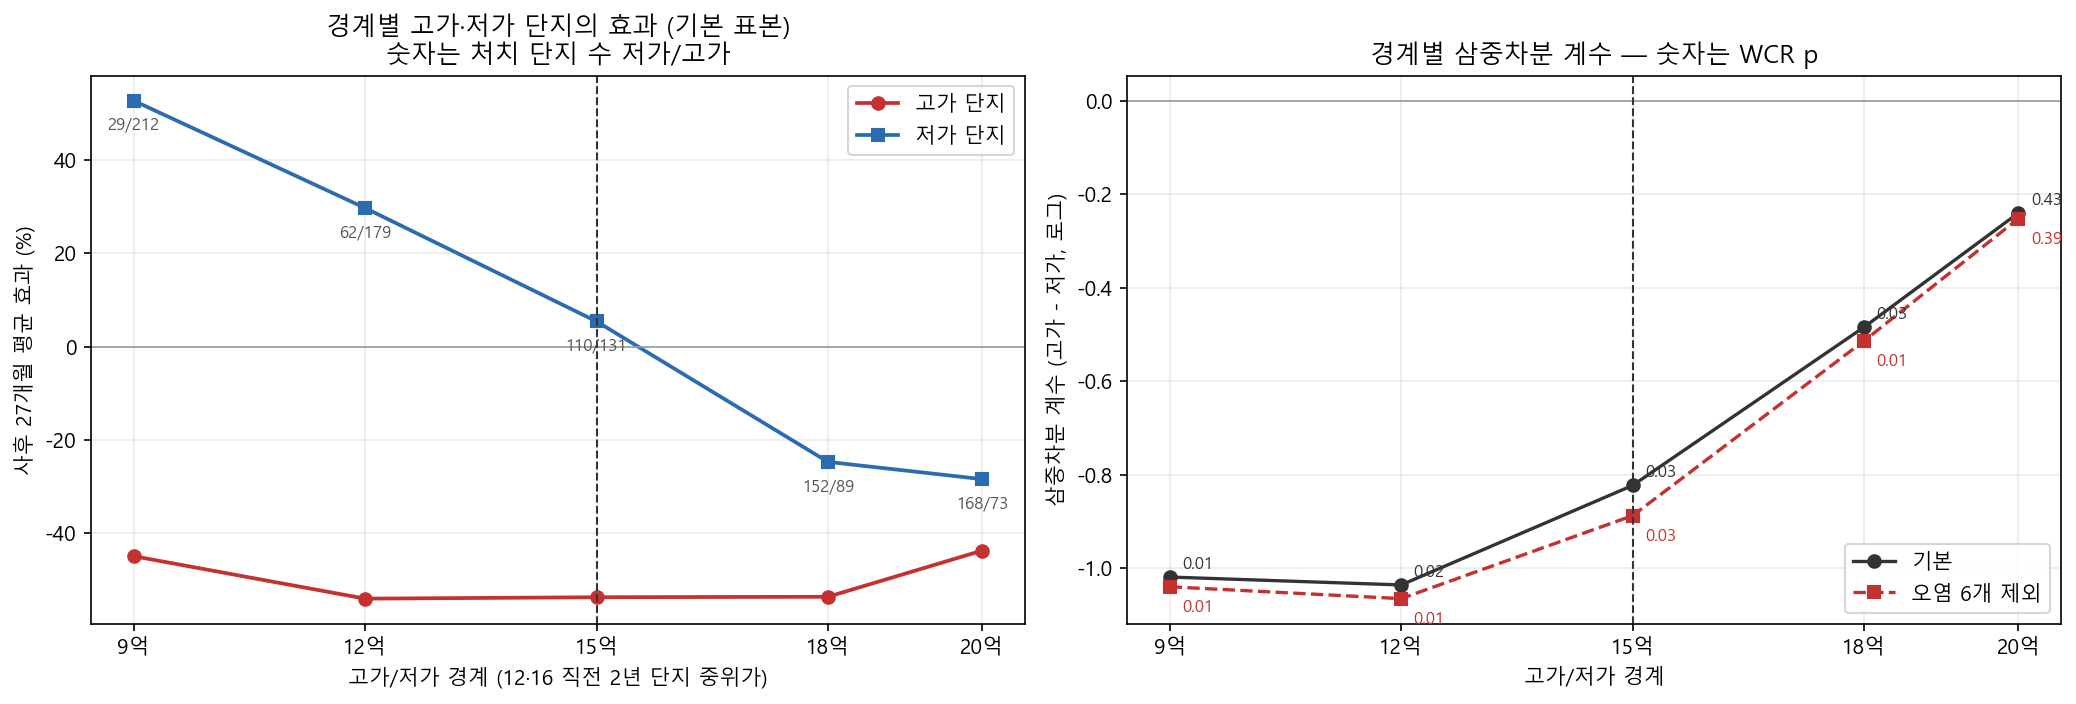
\includegraphics[width=\linewidth]{06f_threshold.png}
  \caption{고가·저가 경계를 9$\sim$20억으로 옮길 때. 15억에 계단이 없다.}
  \label{fig:threshold}
\end{figure}

읽을 것이 셋이다.

\textbf{첫째, 고가 효과는 어느 경계에서나 $-44 \sim -54\%$다.} 15억을 골라서 나온
결과가 아니다. 이 점에서는 2주차 결론이 보강된다.

\textbf{둘째, 저가 효과는 경계를 따라 미끄러진다.} $+52.7\%$에서 $-28.4\%$까지
부드럽게 내려간다. 경계를 올리면 12억·15억짜리 단지가 `저가'로 넘어오는데 그
단지들도 크게 줄었기 때문이다.

\textbf{셋째 --- 그리고 결정적으로 --- 15억에 계단이 없다.} 대출이 이질성을
만들었다면 15억 초과는 대출이 이미 막혀 있었고 15억 이하는 아니었으므로 효과가
15억을 사이에 두고 \textbf{뚝 끊겨야} 한다. 자료는 그렇지 않다. 고가 효과가
12·15·18억에서 $-54.0$, $-53.7$, $-53.6\%$로 평평하다. \textbf{15억은 자료 안에서
특별한 자리가 아니다.}

\subsection{`저가'는 사실상 `소형'이었다}

경계를 낮출수록 `저가'가 무엇과 겹치는지 보았다. \textbf{9억 이하 처치 단지 거래의
전용면적 중위값이 36.4\,m$^2$}다. 9억 초과는 84.8\,m$^2$다.

그리고 2020년 6월 지정의 허가 대상은 \textbf{주거지역 대지 18\,m$^2$ 초과}였다.
대지지분이 작은 소형은 구역 안에 있어도 \textbf{허가 없이 살 수 있었다.}

전용면적대별로 원자료를 보면 모양이 분명하다.

\begin{table}[htbp]
  \centering
  \caption{전용면적대별 거래 변화 (사전 24개월 대비 사후 27개월 월평균)}
  \label{tab:area-raw}
  \begin{tabular}{lrrrr}
    \toprule
    \textbf{전용면적} & \textbf{처치 사전 월평균} & \textbf{처치 변화} &
    \textbf{통제 변화} & \textbf{차이} \\
    \midrule
    \textbf{40\,m$^2$ 미만} & 10.0 & $\mathbf{+7.3\%}$ & $-3.6\%$ &
      $\mathbf{+10.9}$\,\%p \\
    40$\sim$60 & 24.3 & $-73.1\%$ & $-51.2\%$ & $-21.9$\,\%p \\
    60$\sim$85 & 96.2 & $-76.8\%$ & $-50.6\%$ & $-26.2$\,\%p \\
    85$\sim$135 & 42.5 & $-76.3\%$ & $-50.7\%$ & $-25.6$\,\%p \\
    135 이상 & 25.5 & $-65.8\%$ & $-41.4\%$ & $-24.5$\,\%p \\
    \bottomrule
  \end{tabular}
\end{table}

\textbf{40\,m$^2$ 미만만 줄지 않았고, 40\,m$^2$ 이상은 크기와 상관없이
$-22 \sim -26$\,\%p로 거의 같다.} 가장 비싼 135\,m$^2$ 이상과 가장 싼
40$\sim$60\,m$^2$가 같은 폭이다.

\textbf{이 모양은 대출 이야기보다 면적 면제 이야기에 맞는다.} 대출이 원인이면
40\,m$^2$ 이상 \emph{안에서도} 비쌀수록 더 줄어야 하는데 그렇지 않다. 면제가
원인이면 면제된 소형만 빠지고 나머지는 같게 줄어야 하는데 그렇다.

\subsection{2022년 기준 강화가 두 가설을 갈랐다}

여기까지는 탐색이다. 두 가설이 \textbf{반대 방향을 예측하는 사건}이 자료 안에
있었다(0022).

\begin{table}[htbp]
  \centering
  \caption{두 가설이 예측하는 것}
  \label{tab:two-hyp}
  \begin{tabular}{lll}
    \toprule
    \textbf{가설} & \textbf{규제가 다르게 물린 축} & \textbf{예측} \\
    \midrule
    대출 & 가격 & 15억을 사이에 두고 효과가 끊긴다 \\
    \textbf{면제} & \textbf{크기} &
      소형만 빠지고, 면제가 사라지면 소형도 줄어든다 \\
    \bottomrule
  \end{tabular}
\end{table}

\textbf{2022년 6월 23일에 허가 기준이 대지 18\,m$^2$에서 6\,m$^2$로 강화됐다}
(서울특별시공고 제2022-1795호 원문에서 확인). 이날 처치 4개 동의 \textbf{소형만}
새로 허가 대상이 된다. 대형은 이미 대상이었으므로 바뀌는 것이 없다.
\textbf{대출 가설은 이 날짜에 아무것도 예측하지 않는다.}

% 자동 생성 — scripts/build_tables.py. 손으로 고치지 않는다.
% 출처: output/results/06g_area_exemption.json : 나_2022_기준강화
\begin{table}[htbp]
  \centering
  \caption{2022-06-23 허가 면적 기준 강화(대지 18 $\to$ 6\,m$^2$). 소형만 줄었다.}
  \label{tab:area-2022}
  \begin{tabular}{lrrrrr}
    \toprule
    \textbf{소형 경계 (m$^2$)} & \textbf{처치 소형 거래} & \textbf{소형 (\%)} & \textbf{대형 (\%)} & \textbf{WCR $p$} & \textbf{무작위화 $p$} \\
    \midrule
    30 & 62 & -26.2 & 17.1 & 0.082 & 0.111 \\
    40 & 130 & -33.2 & 21.7 & 0.021 & 0.016 \\
    50 & 141 & -30.9 & 21.0 & 0.022 & 0.055 \\
    60 & 212 & -19.8 & 12.1 & 0.123 & 0.108 \\
    \bottomrule
  \end{tabular}

  \begin{minipage}{\linewidth}\footnotesize
  \textit{주.} 그날 처치동 소형만 새로 허가 대상이 된다. 대출 가설은 이 날짜에 아무것도 예측하지 않는다.
  \end{minipage}
\end{table}


\begin{figure}[htbp]
  \centering
  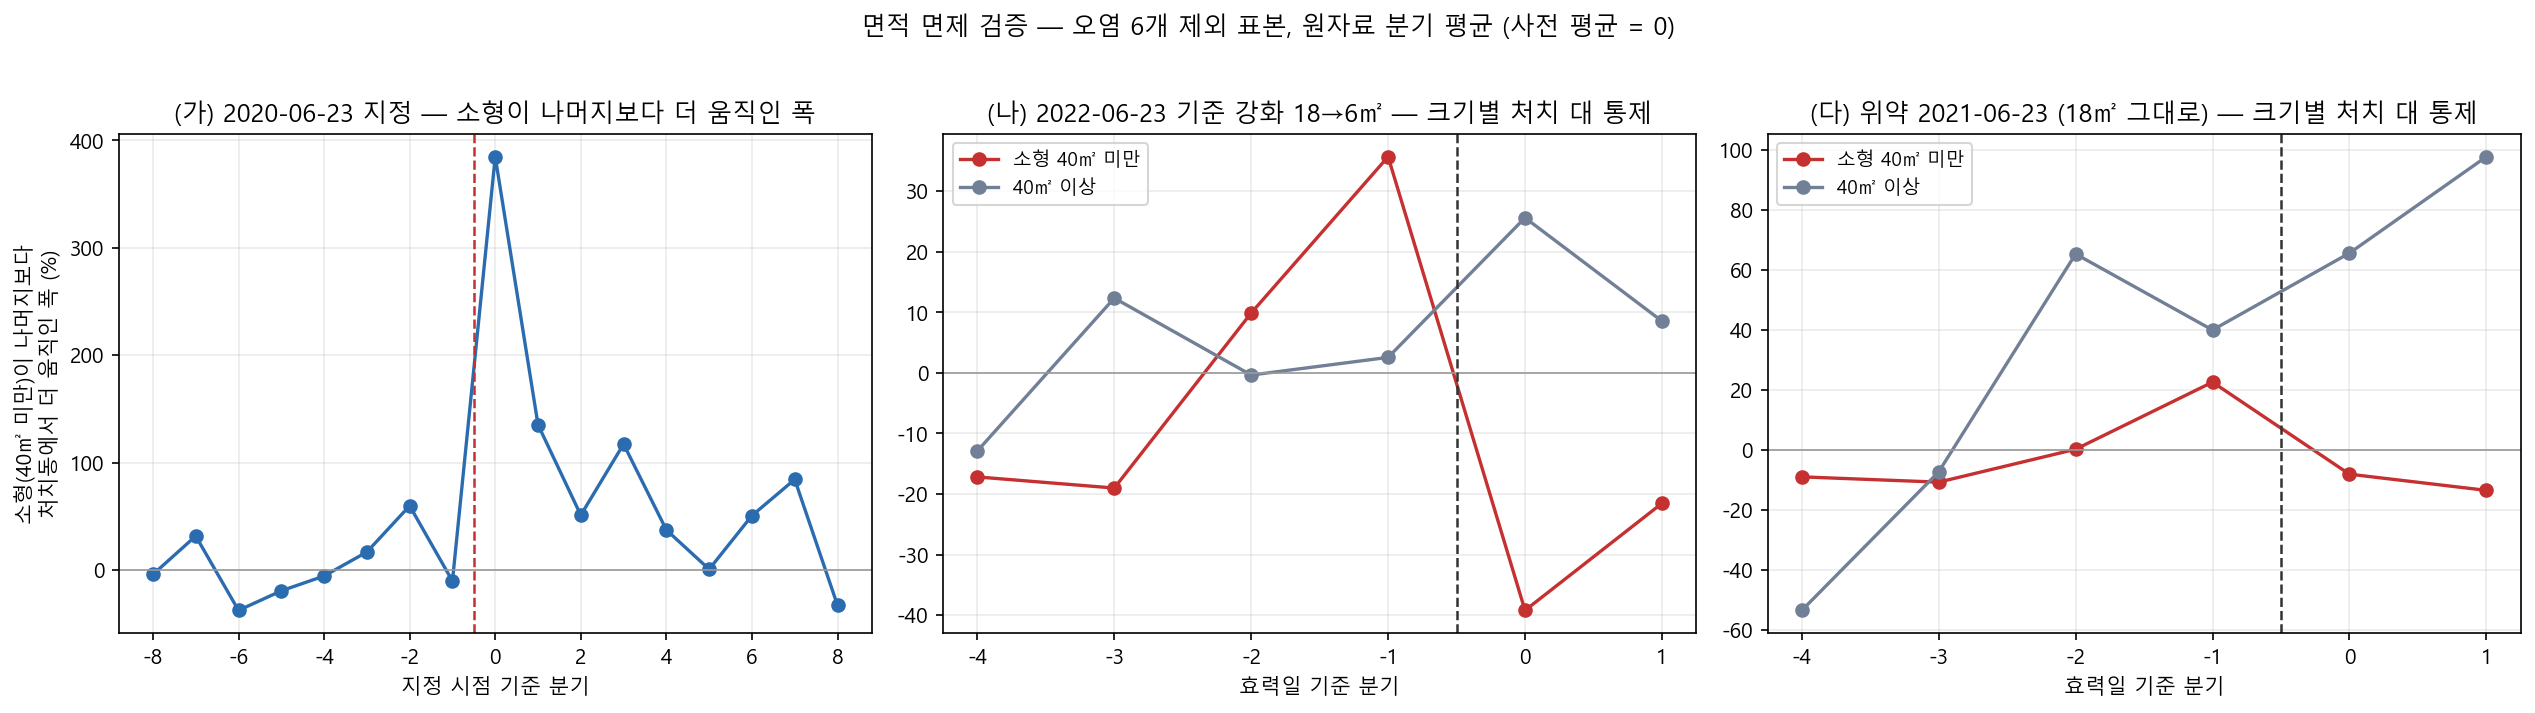
\includegraphics[width=\linewidth]{06g_area_exemption.png}
  \caption{면적 면제 검증. 가운데가 2022년 기준 강화, 오른쪽이 2021년 위약.
           빨간 선이 소형(40\,m$^2$ 미만)이다.}
  \label{fig:area-exemption}
\end{figure}

\textbf{소형만 줄었다.} 40\,m$^2$ 경계에서 $-33.2\%$(WCR 0.023, 무작위화 0.001)이고
\textbf{대형은 오히려 올라간다}($+21.7\%$, 0.236).

\textbf{첫 설계는 위약에서 실패했음을 밝혀 둔다.} 처음에는 처치동 소형과 처치동
대형을 견주는 삼중차분으로 했는데, 2021년 위약이 $-0.715$로 진짜($-0.600$)만큼
크게 나왔다. 원인은 비교 기준이었다 --- 2021년 위약의 사전 구간은 2020년 지정 직후
1년이라 처치동 대형이 폭락해 있던 때이고, 사후에 대형이 회복하니 ``소형이
상대적으로 줄었다''로 보였다. \textbf{대형을 비교 기준에서 빼고 같은 크기끼리
처치동 대 통제동으로 다시 쟀다.}

\subsection{위약 --- 2021년 재지정}

2021년 6월 23일 재지정은 같은 계절, 같은 행정 절차였지만 \textbf{면적 기준을
18\,m$^2$ 그대로 두었다.} 소형에게 바뀐 것이 없으므로 효과가 0이어야 한다.

% 자동 생성 — scripts/build_tables.py. 손으로 고치지 않는다.
% 출처: output/results/06g_area_exemption.json : 다_2021_위약
\begin{table}[htbp]
  \centering
  \caption{위약 --- 2021-06-23 재지정. 면적 기준을 그대로 두었다.}
  \label{tab:area-2021}
  \begin{tabular}{lrrrr}
    \toprule
    \textbf{소형 경계 (m$^2$)} & \textbf{소형 (\%)} & \textbf{대형 (\%)} & \textbf{WCR $p$} & \textbf{무작위화 $p$} \\
    \midrule
    30 & -14.5 & 72.0 & 0.009 & 0.009 \\
    40 & -8.1 & 87.8 & 0.016 & 0.011 \\
    50 & 6.2 & 84.2 & 0.025 & 0.038 \\
    60 & 20.7 & 83.2 & 0.034 & 0.047 \\
    \bottomrule
  \end{tabular}

  \begin{minipage}{\linewidth}\footnotesize
  \textit{주.} 같은 계절, 같은 행정 절차인데 소형에 바뀐 것이 없다. 0 이어야 한다.
  \end{minipage}
\end{table}


\textbf{소형은 규칙이 바뀐 해에만 줄었다.} 2021년에는 $-8.1\%$($p=0.61$)로 0과
구분되지 않고, 2022년에는 $-33.2\%$($p=0.023$)다. 직전 분기를 빼도 $-27.4\%$가
남고, 사전 24개월로 늘려도 $-32.1\%$다. 소형 경계를 옮겨도 30\,m$^2$ $-26\%$,
40 $-33\%$, 50 $-31\%$, 60 $-20\%$로 유지된다(60에서 약해지는 것은 대지 18\,m$^2$를
넘는 단지가 섞여 들어오기 때문으로 읽는다).

\textbf{소형을 빼면 15억 가격 차이가 유의하지 않아진다.} 전체 표본에서 차이가
$-0.823$(무작위화 0.037)인데 40\,m$^2$ 이상만 남기면 $-0.669$(무작위화
\textbf{0.098})가 된다. \textbf{가격 차이의 상당 부분이 소형이었다.}

\subsection{사전 등록한 예측이 맞았다}

4.7절에 적어 둔 예측을 확인할 차례다. 2025년 2월 13일 A그룹이 대부분 해제됐다가
\textbf{39일 만인 3월 24일} 강남3구·용산 전체 아파트로 재지정됐다. 이번 지정의
허가 기준은 \textbf{6\,m$^2$}이므로 소형 면제가 거의 없다.

% 자동 생성 — scripts/build_tables.py. 손으로 고치지 않는다.
% 출처: output/results/09_release_2025.json : 크기_삼중차분
\begin{table}[htbp]
  \centering
  \caption{면적 기준이 바뀌자 효과의 모양이 바뀌었다. 2022년에 적어 둔 예측이 2025년 자료에서 확인됐다.}
  \label{tab:size-ddd}
  \begin{tabular}{lrrrrr}
    \toprule
    \textbf{사건} & \textbf{허가 대상} & \textbf{대형 (\%)} & \textbf{소형 (\%)} & \textbf{차이 (로그)} & \textbf{$p$} \\
    \midrule
    2020-06-23 지정 & 대지 18㎡ 초과 & -95.0 & 125.7 & 3.818 & $<0.001$ \\
    2025-03-24 재지정 & 대지 6㎡ 초과 & -89.4 & -71.5 & 0.987 & 0.388 \\
    \bottomrule
  \end{tabular}

  \begin{minipage}{\linewidth}\footnotesize
  \textit{주.} 2020년 지정은 대지 18\,m$^2$ 초과만 허가 대상이라 소형이 면제됐고, 2025년 재지정은 6\,m$^2$ 라 면제가 거의 없다.
  \end{minipage}
\end{table}


\begin{figure}[htbp]
  \centering
  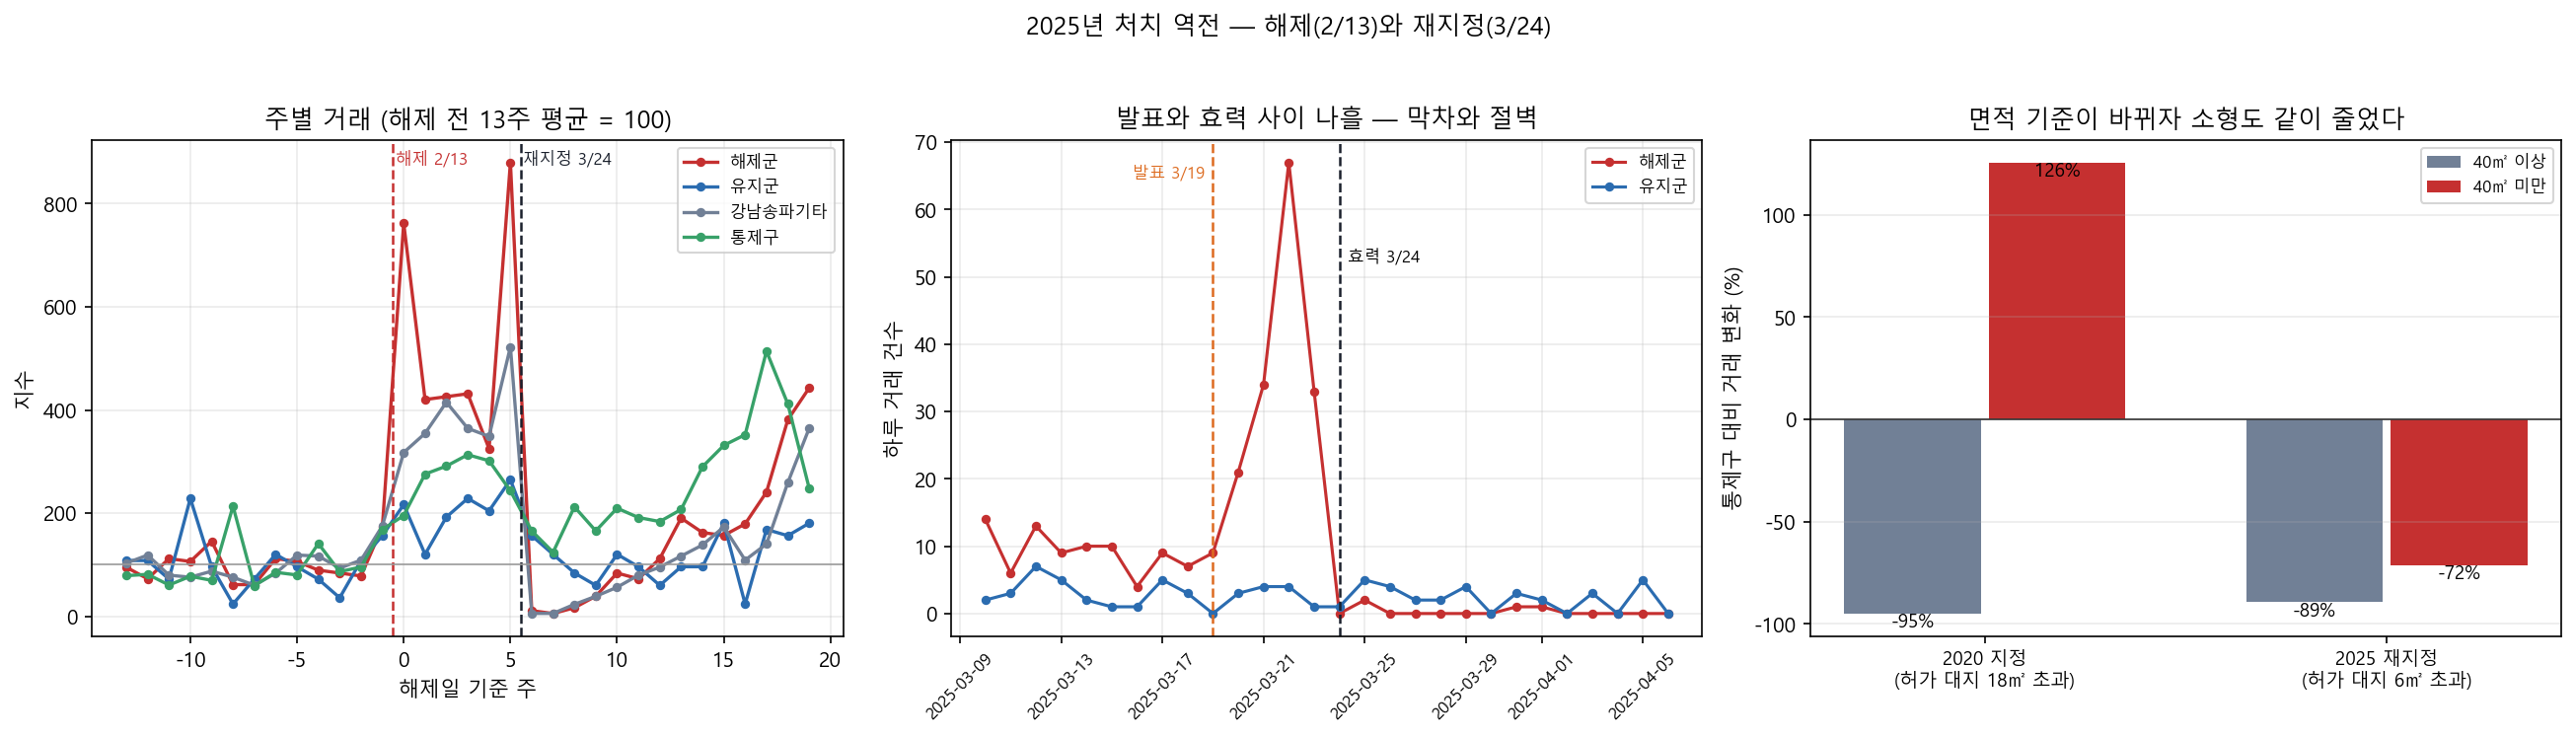
\includegraphics[width=\linewidth]{09_release_2025.png}
  \caption{2025년 처치 역전. 왼쪽 주별 거래, 가운데 발표와 효력 사이 나흘의
           막차와 절벽, 오른쪽 면적 기준이 바뀌자 소형도 줄었다.}
  \label{fig:release-2025}
\end{figure}

\textbf{예측이 맞았다.} 2020년에는 대형 $-95.0\%$ 대 소형 $+125.7\%$로 부호가
반대였는데, 2025년에는 대형 $-89.4\%$ 대 소형 $-71.5\%$로 \textbf{같은 방향}이다.
두 집단의 차이가 2020년 $+3.818$에서 2025년 $+0.987$로 줄었다.

재지정 직후 5주 거래량은 유지군 대비 $-78.9\%$이고(정상 13주 기저), 해제창을
기저로 하면 $-92.3\%$다. 12주로 늘리면 통제군에 따라 $-14\%$와 $-60\%$로 갈리므로
\textbf{지속 기간은 여기서도 말하지 않는다.}

그림 가운데 패널이 덤으로 나온 발견이다. 공고(3월 19일)와 효력(3월 24일) 사이
\textbf{나흘} 동안 하루 거래가 평소 5$\sim$10건에서 \textbf{66건}까지 튀었다가
효력일 다음 날부터 0 근처로 떨어진다. 주간으로 보면 30$\to$155$\to$2건이다.
\textbf{막차 수요가 하루 단위 자료에서만 보인다.} 그리고 그 막차 계약이 나중에
무더기로 취소된 것도 아니다 --- 2020년 막차 구간의 취소율이 3.78\%로 직전 한 달
4.85\%보다 오히려 낮다(9.7절).

\subsection{대출의 몫 --- 작거나 가릴 수 없다}

면적 기준이 주된 원인이라는 결론이 \textbf{대출의 몫이 0이라는 뜻은 아니다.}
소형을 뺀 뒤에도 15억 경계의 차이가 점추정으로 $-0.669$ 남는다. 무작위화로는
유의하지 않다(0.098).

대출 가설을 한 번 더 걸어 보려고 \textbf{15억 금지의 폐지}(2022-12-01)를 사건으로
삼았다(0029). 걸 때 줄었다면 풀 때 돌아와야 한다. \textbf{착수 전에 교란 셋을
적어 두었고 셋 다 현실로 나타났다} --- 그날 9억 꺾임도 함께 풀렸고, 한 달 뒤
2023-01-03 대책이 규제지역을 대거 해제했으며, 2022년 말은 금리 급등기였다.

\begin{table}[htbp]
  \centering
  \caption{금지와 폐지의 거울상 (고가 단지 거래, 저가 대비)}
  \label{tab:mirror}
  \begin{tabular}{lrrr}
    \toprule
    \textbf{사건} & \textbf{$\pm$1개월} & \textbf{$\pm$3개월} &
    \textbf{$\pm$12개월} \\
    \midrule
    2019-12-17 금지 & $-32.2\%$ (0.001) & $-50.7\%$ ($<0.001$) &
      $-33.5\%$ ($<0.001$) \\
    2022-12-01 폐지 & $+21.3\%$ (\textbf{0.380}) & $+81.1\%$ ($<0.001$) &
      $+67.7\%$ ($<0.001$) \\
    \bottomrule
  \end{tabular}
\end{table}

부호가 반대이고 위약도 깨끗하다(2020-12-01 $+0.6\%$, 2021-12-01 $-9.1\%$,
2023-12-01 $+5.1\%$). \textbf{그러나 1·3 대책 이전의 깨끗한 창($\pm$1개월)에서는
유의하지 않다.} 그리고 문턱을 옮기면 폐지 효과가 9억 $+123.9\%$에서 20억
$+69.5\%$로 매끈하게 기울며 \textbf{15억에 아무 일도 일어나지 않는다.}

\begin{figure}[htbp]
  \centering
  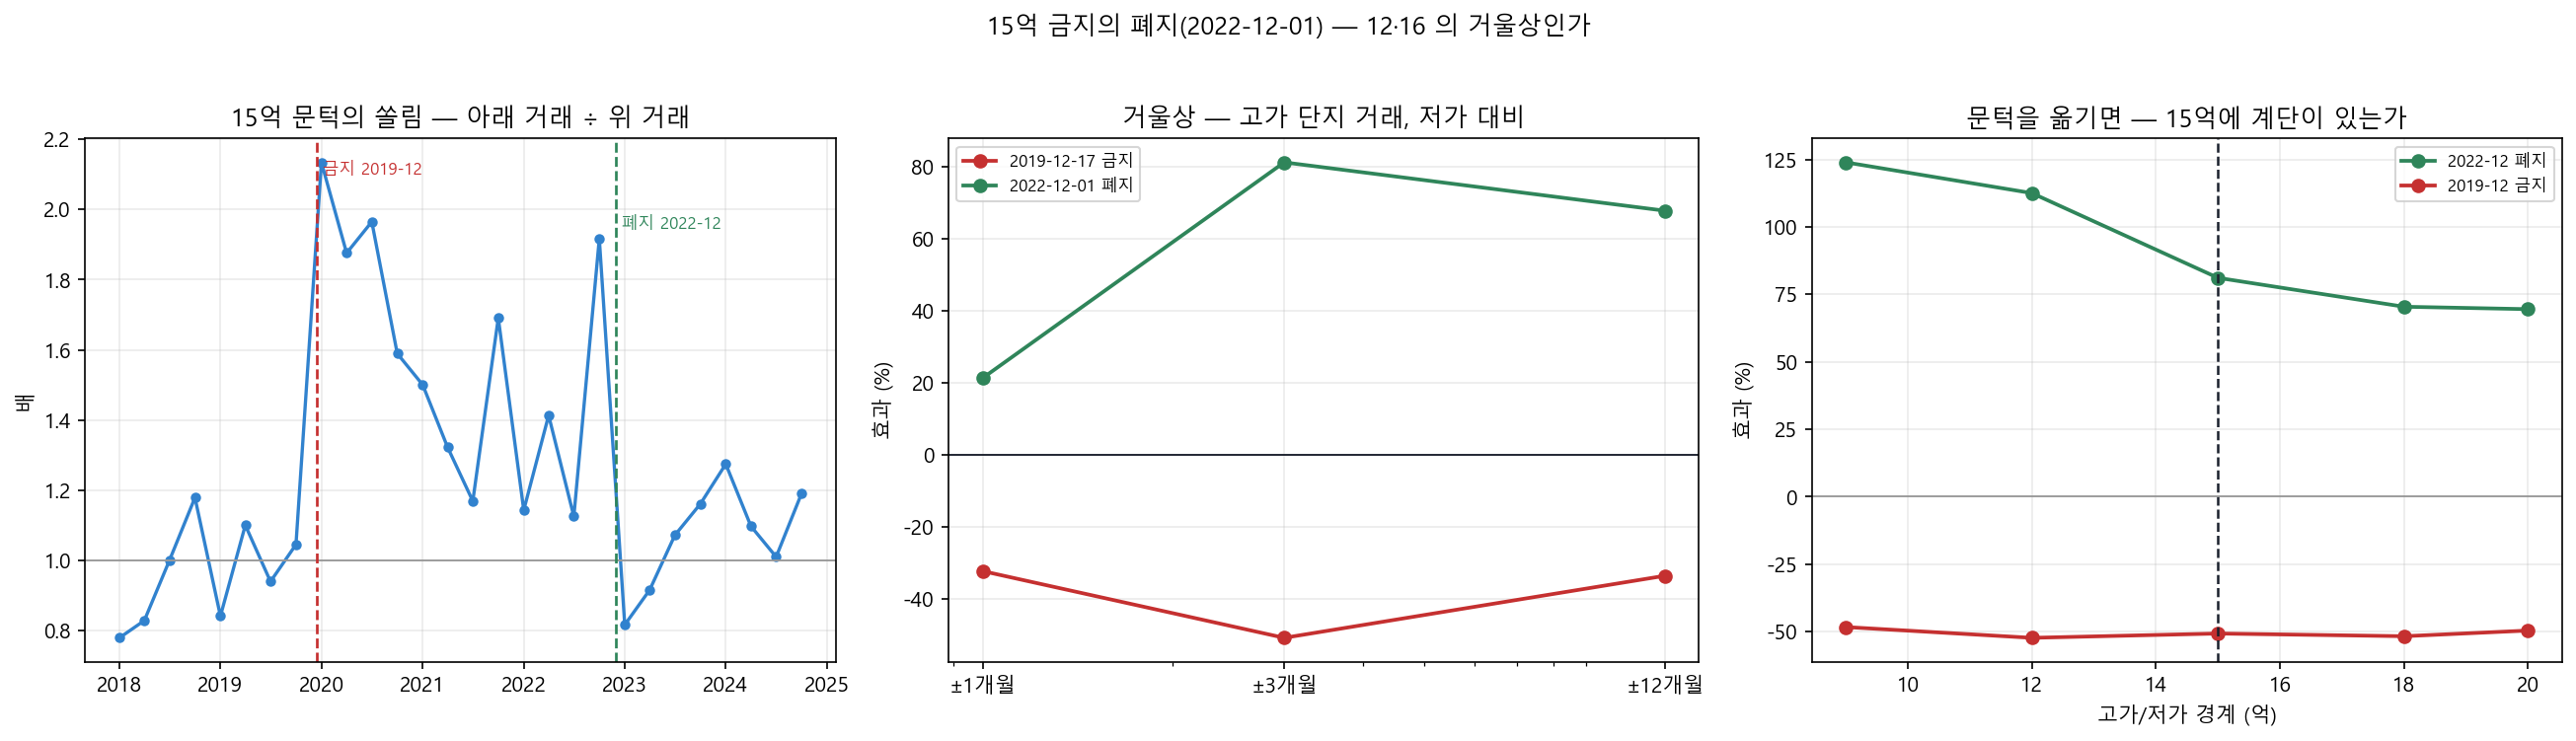
\includegraphics[width=\linewidth]{06e_loan_repeal.png}
  \caption[15억 금지(2019-12)와 그 폐지(2022-12-01) --- 15억에 계단이 없다]{%
    15억 금지(2019-12)와 그 폐지(2022-12-01). \textbf{오른쪽 판이 이
    절의 요지다} --- 가로축을 고가/저가 경계로 삼아 문턱을 9억에서 20억까지
    옮겨도 두 선 모두 \textbf{15억(점선)에서 꺾이지 않는다}. 규제가 15억에
    걸려 있는데 효과가 15억에서 계단을 만들지 않는다면, 그 효과를 대출 규제의
    몫으로 돌릴 수 없다(0021 · 0029). 가운데 판은 금지와 폐지의 부호가 반대라는
    것을, 왼쪽 판은 문턱 아래위 거래 비율이 금지 시점에 2.1배까지 치솟았다가
    폐지 시점에 되돌아오는 것을 보여 준다.}
  \label{fig:loan-repeal}
\end{figure}

\textbf{``폐지 덕에 고가 거래가 돌아왔다''고 쓰지 않는다.} 돌아온 것은 사실이지만
금리 정점 통과와 1·3 대책에서 그 몫을 가를 수 없다. 이 작업의 수확은 오히려
\textbf{``15억에 계단이 없다''를 서울 전역·다른 사건·다른 창에서 재확인}한 것이다.
6.4절은 강남·송파 표본 하나였다.

\subsection{이 장의 결론}

\begin{quote}
대출 규제는 \textbf{교란변수가 아니다}. 토지거래허가제의 효과는 단지마다
달랐는데, 그 차이는 대출 규제보다 \textbf{허가 대상의 면적 기준}으로 더 잘
설명된다. 2020년에는 대지 18\,m$^2$ 이하 소형이 허가 대상에서 빠져 거래가 줄지
않았고, 2022년 기준이 6\,m$^2$로 강화되자 그 소형의 거래가 약 3분의 1 줄었다.
\textbf{대출의 몫은 작거나 가릴 수 없다.}
\end{quote}

근거는 셋이다. 2020년 지정 때 소형은 줄지 않았고, 2022년 기준이 강화되자
\emph{그때} 소형이 줄었으며, 기준을 바꾸지 않은 2021년 재지정에서는 소형이
움직이지 않았다. \textbf{대출 가설은 뒤의 둘을 설명하지 못한다.}

% 7장 어디로 번졌나. 0024

\section{어디로 번졌나}

토허제의 명분은 가격 안정이다. 규제 밖 단지로 수요가 옮겨 갔을 뿐이라면 규제는
문제를 푼 것이 아니라 \textbf{옮긴 것}이다. 선행연구 두 편이 `인근 지역 급등'을
보고했다\citep{lee2025, yang2025}.

\subsection{규제 밖이 세 층으로 있다}

이 자료에는 규제 밖이 세 층으로 있고 \textbf{층마다 사건이 다르다}(0024).

\begin{table}[htbp]
  \centering
  \caption{규제 밖의 세 층}
  \label{tab:spill-layers}
  \begin{tabular}{llp{6.5cm}}
    \toprule
    \textbf{층} & \textbf{사건} & \textbf{규제 밖에 무엇이 있나} \\
    \midrule
    1 같은 동 안 & 2025-02-13 해제 & 해제군 옆에 유지군 16개 단지가 남았다 \\
    2 옆 동 & 2020-06-23 지정 & 처치 4개 동에 11개 동이 맞닿는다 \\
    3 옆 구 & 2025-03-24 재지정 & 강남3구·용산이 막히고 4개 구가 남았다 \\
    \bottomrule
  \end{tabular}
\end{table}

\textbf{층 1이 이 연구의 특별한 조건이다.} 통상적인 파급효과 연구는 규제 지역과
인접한 비규제 지역을 비교하므로 두 지역이 원래 달랐을 가능성이 남는다. 2025년
2월 해제는 전면적이 아니라 부분적이어서 \textbf{같은 동 안에 규제 상태가 다른
단지가 공존}한다. 학군·교통·생활권이 물리적으로 동일하다.

맞닿은 동은 법정동 경계 다각형(467개)으로 뽑는다. 처치 4개 동 덩어리에 닿는 동이
14개이고, 창 안에 다른 계열로 지정된 동을 빼면 11개가 남는다.

\textbf{기준점을 명시하는 것이 이 장의 핵심이다.} 파급을 `처치동 대비'로 재면
처치동이 줄어든 것만으로도 옆 동이 늘어난 것처럼 보인다. 같은 자료·같은 창에
기준점만 바꿔 가며 사다리를 만들어 함께 싣는다.

\subsection{같은 동 안에서만 옮겨 갔다}

파급이 있으면 \textbf{규제가 바뀐 쪽과 안 바뀐 쪽의 부호가 반대}여야 한다. 한쪽이
늘 때 다른 쪽이 줄었으면 수요가 옮겨 간 것이고, 둘 다 줄었으면 같이 영향받은 것이다.

\begin{table}[htbp]
  \centering
  \caption{규제가 바뀐 쪽과 안 바뀐 쪽 (거래량). 층마다 사건이 다르다}
  \label{tab:spill-pairs}
  \begin{tabular}{llrr}
    \toprule
    \textbf{규제 밖이 어디에} & \textbf{사건} &
    \textbf{규제가 바뀐 쪽} & \textbf{안 바뀐 쪽} \\
    \midrule
    \textbf{같은 동 안} & 2025.2 해제 &
      해제군 $+80.6\%$ & 유지군 $\mathbf{-26.5\%}$ \\
    옆 동 & 2020.6 지정 &
      처치동 $-57.8\%$ & 맞닿은 동 $-9.0\%$ \\
    옆 구 & 2025.3 재지정 &
      강남3구·용산 $-82.3\%$ & 인접 4개 구 $+23.0\%$ (0.16) \\
    \bottomrule
  \end{tabular}
\end{table}

\textbf{같은 동 안에서는 옮겨 갔다.} 2025년 2월에 규제가 대부분 풀렸는데 16개
단지만 그대로 남았다. 풀린 쪽이 $+80.6\%$, \textbf{규제가 하나도 바뀌지 않은
유지군이 $-26.5\%$}다($p<0.001$, 먼 통제군 대비). 같은 동, 같은 학군, 같은 달인데
바뀐 것은 \textbf{옆 단지의 규제가 풀렸다는 것뿐}이다.

\textbf{옆 동으로는 가지 않았다.} 2020년 지정에서 맞닿은 동이 $-9.0\%$($p=0.088$)로
\textbf{늘어난 것이 아니라 같이 줄었다.} 공통지지 표본에서는 $-19.0\%$로 더
내려간다.

% 자동 생성 — scripts/build_tables.py. 손으로 고치지 않는다.
% 출처: output/results/12_spillover.json : 층2_고리별
\begin{table}[htbp]
  \centering
  \caption{2020-06 지정의 거리 고리별 효과. 서울 나머지 19개 구 대비.}
  \label{tab:spill-rings}
  \begin{tabular}{lrrrr}
    \toprule
    \textbf{고리} & \textbf{거래량 (\%)} & \textbf{$p$} & \textbf{가격 (\%)} & \textbf{$p$} \\
    \midrule
    R0 처치동 & -57.8 & $<0.001$ & -9.7 & $<0.001$ \\
    R1 맞닿은 동 & -9.0 & 0.088 & -5.0 & 0.001 \\
    R2 강남송파 비인접 & -2.4 & 0.664 & -1.5 & 0.269 \\
    R3 인접 4개구 & -10.4 & 0.055 & -0.7 & 0.459 \\
    \bottomrule
  \end{tabular}

  \begin{minipage}{\linewidth}\footnotesize
  \textit{주.} 어느 고리도 거래량이 양($+$)이 아니다. 거래가 옆 동으로 옮겨 간 흔적이 없다.
  \end{minipage}
\end{table}


\begin{figure}[htbp]
  \centering
  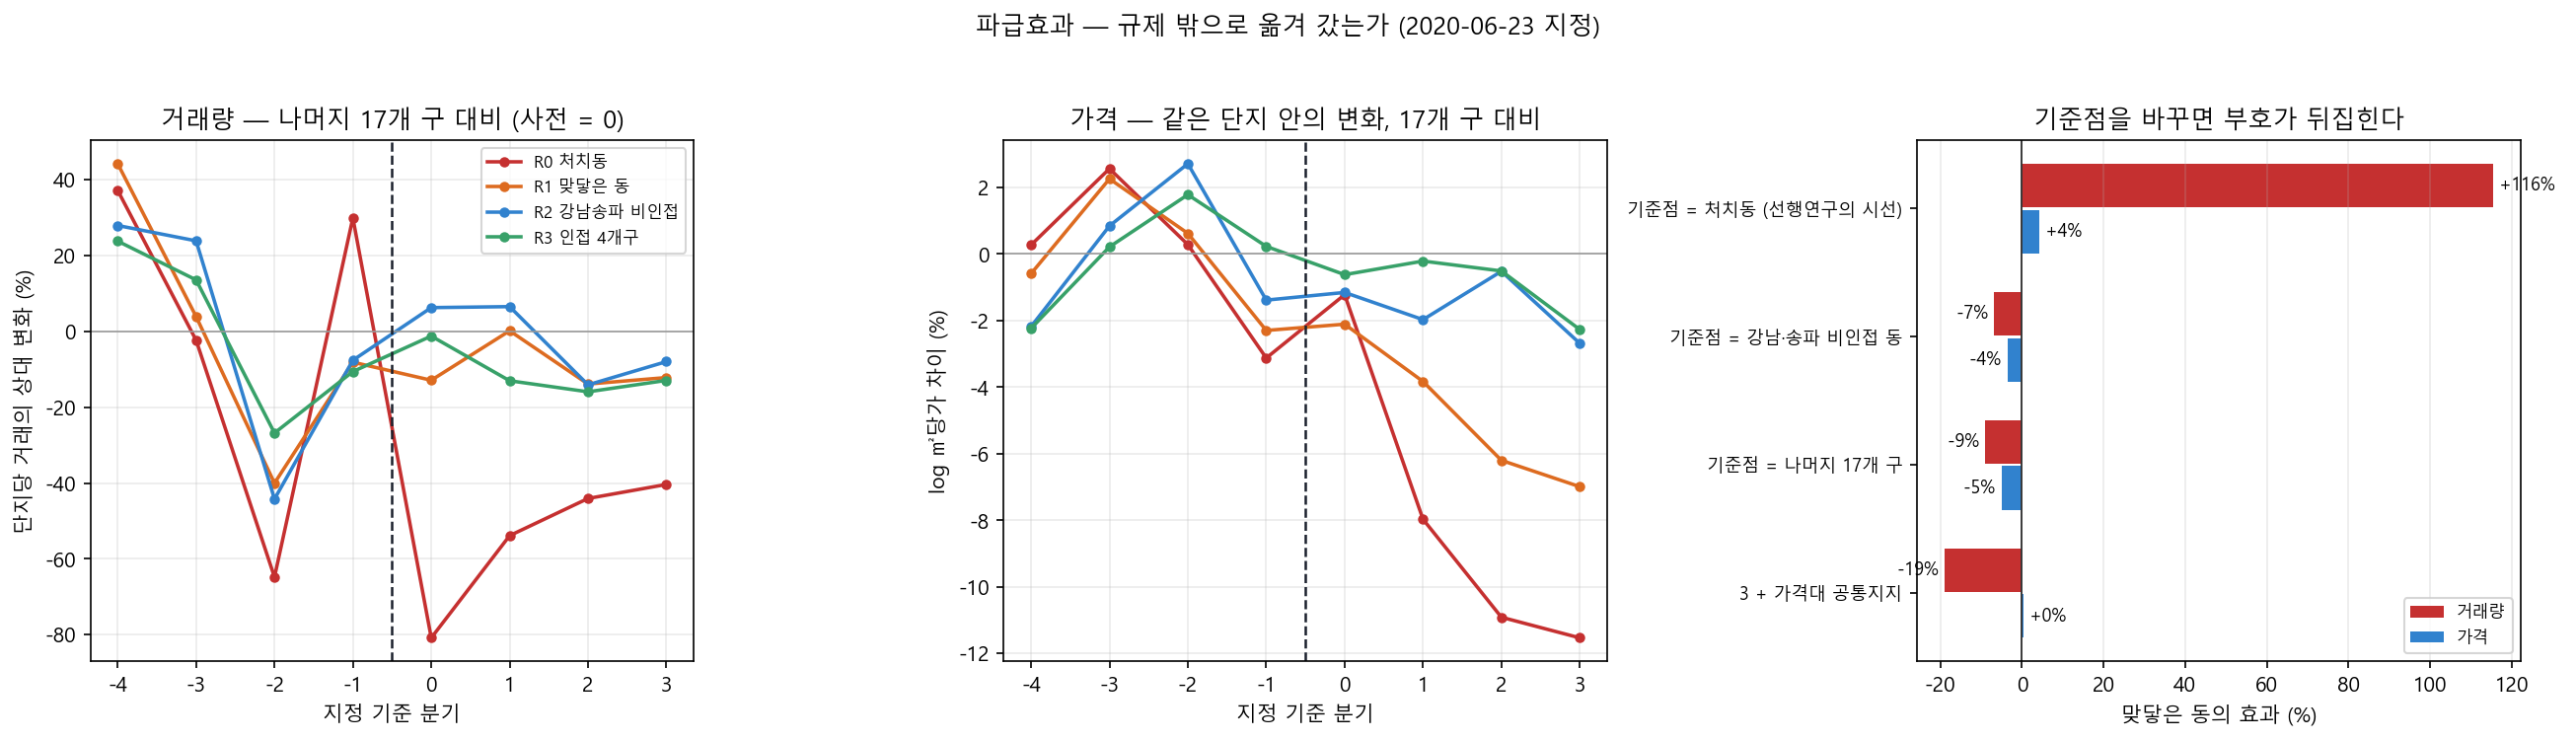
\includegraphics[width=\linewidth]{12_spillover.png}
  \caption{파급효과. 왼쪽 거리 고리별 거래량, 가운데 가격, 오른쪽 기준점을
           바꾸면 부호가 뒤집힌다.}
  \label{fig:spillover}
\end{figure}

\textbf{옆 구는 방향만 있다.} 2025년 재지정에서 인접 4개 구가 $+23.0\%$로 부호는
파급 방향이지만 $p=0.157$이다. 창이 5주로 짧고 늘리면 2025-06-27 대출 규제가
섞인다. \textbf{``인접 구로 넘어갔다''고 쓰지 않는다.} 같은 `인접 4개 구'가 2020년
사건에서는 $-10.4\%$로 부호가 반대인 것도 단정하지 말아야 할 이유다.

\textbf{여기서 `유의하지 않다'를 `효과가 없다'로 읽으면 안 된다.} 창이 5주라 검정력이
모자란 것인지 효과가 없는 것인지 가를 수 없다. \textbf{``확인할 수 없다''}로 쓴다.

\subsection{기준점을 바꾸면 부호가 뒤집힌다}

이 절이 7장에서 가장 중요하다. 아래 표는 \textbf{같은 맞닿은 동}이고 같은 자료,
같은 창, 같은 사양이다. \textbf{무엇과 견주는지만} 다르다.

% 자동 생성 — scripts/build_tables.py. 손으로 고치지 않는다.
% 출처: output/results/12_spillover.json : 사다리_맞닿은동
\begin{table}[htbp]
  \centering
  \caption{같은 자료, 같은 창, 같은 사양. 기준점만 바꿨다 (맞닿은 동).}
  \label{tab:spill-bench}
  \begin{tabular}{lrrrr}
    \toprule
    \textbf{기준점} & \textbf{거래량 (\%)} & \textbf{$p$} & \textbf{가격 (\%)} & \textbf{$p$} \\
    \midrule
    1. 기준점 = 처치동 (선행연구의 시선) & 115.5 & $<0.001$ & 4.3 & 0.111 \\
    2. 기준점 = 강남·송파 비인접 동 & -6.8 & 0.331 & -3.6 & 0.055 \\
    3. 기준점 = 나머지 19개 구 & -9.0 & 0.088 & -5.0 & 0.001 \\
    4. 3 + 가격대 공통지지 & -19.0 & 0.021 & 0.3 & 0.748 \\
    \bottomrule
  \end{tabular}

  \begin{minipage}{\linewidth}\footnotesize
  \textit{주.} $+115.5\%$ 는 옆 동이 늘어서가 아니라 처치동이 $-57.8\%$ 로 줄어서다. 선행연구가 보고한 `인근 급등' 이 이것이다.
  \end{minipage}
\end{table}


\textbf{처치동과 견주면 $+115.5\%$, 서울 나머지 19개 구와 견주면 $-9.0\%$다.}
맞닿은 동의 거래가 처치동보다 116\% 많아진 것은 \textbf{사실}이다. 그런데 그것은
옆 동이 늘어서가 아니라 \textbf{처치동이 57.8\% 줄어서}다. 분모가 반 토막 나면
가만히 있어도 상대적으로 두 배가 된다.

\subsection{선행연구의 `인근 급등'을 다시 읽는다}

\textbf{선행연구 두 편이 보고한 `인근 지역 급등'이 표~\ref{tab:spill-bench}의
첫 줄이다.} 계산이 틀린 것이 아니다. 기준점이 처치동일 뿐이다.

\begin{quote}
``토허제 때문에 인근이 급등했다''는 말은 \textbf{처치동을 기준으로 봤을 때만
참이다.} 기준점을 서울 전체로 한 칸만 옮기면 $-9.0\%$가 된다.
\end{quote}

처치동으로 같은 사다리를 놓으면 거래량은 기준점을 어떻게 바꿔도
$-57 \sim -64\%$다. \textbf{처치 효과는 기준점에 둔감하고 파급 효과는 민감하다.}
파급을 보고할 때 기준점을 밝히지 않으면 같은 자료에서 정반대 결론이 나온다는
것이 이 장의 방법론적 교훈이다.

그리고 \textbf{층을 가로질러 크기를 비교하지 않는다.} 창 길이부터 다르다 ---
2020년 사건은 $\pm$12개월, 2025년 사건은 전 13주·후 5주다. 어느 층의 숫자가 더
큰지 견주는 것은 뜻이 없다.

% 8장 가격은 잡혔나. 0001 · 0003 · 0018 · 0025 · 0026

\section{가격은 잡혔나}

토허제의 명분이 가격 안정이므로 이 장이 제도 평가의 직접적인 자리다. 결론을 먼저
적으면 \textbf{가격을 잡았다는 증거는 약하다.}

\subsection{구성 변화 문제}

거래가 80\% 줄면 \textbf{팔리는 집의 종류가 바뀐다.} 어느 동의 한 달 평균 가격은
그달에 팔린 집들의 평균이므로, 각 단지의 가격이 하나도 변하지 않아도 어떤 단지가
더 많이 팔렸느냐에 따라 평균이 움직인다. 측정된 ``평균 가격 변화'' 안에
\textbf{진짜 가격 변화 + 구성 변화}가 섞인다.

구성이 실제로 바뀌었다. 처치동 사후 표본의 평균 전용면적이 93.9\,m$^2$에서
88.7\,m$^2$로 이동했고, 2020년 9월에는 처치 4개 동의 월평균 전용면적이
103.4\,m$^2$로 튀면서 그달의 중위가 지수(170.5)와 반복매매지수(159.4)가
\textbf{11포인트} 벌어졌다.

\subsection{지수 다섯의 사다리}

구성 통제의 사다리로 같은 자료에 지수 다섯을 지었다(3.4절, 0025). 아래로 갈수록
더 많은 것을 고정한다. 지정 전후 12개월, 처치동 $\div$ 통제동 비의 변화다.

\begin{table}[htbp]
  \centering
  \caption{무엇을 고정하느냐에 따라 가격 효과가 절반이 된다}
  \label{tab:price-ladder}
  \begin{tabular}{llr}
    \toprule
    \textbf{가격지수} & \textbf{무엇을 고정하나} & \textbf{12개월 변화} \\
    \midrule
    중위가 (총액) & 아무것도 & $-10.1\%$ \\
    중위가 (㎡당) & 물건의 크기 & $-12.5\%$ \\
    헤도닉 & 면적과 층 & $-11.1\%$ \\
    \textbf{헤도닉 + 단지} & 거기에 단지의 질까지 & $\mathbf{-5.9\%}$ \\
    \textbf{반복매매} & 같은 집 & $\mathbf{-6.0\%}$ \\
    \bottomrule
  \end{tabular}
\end{table}

\begin{figure}[htbp]
  \centering
  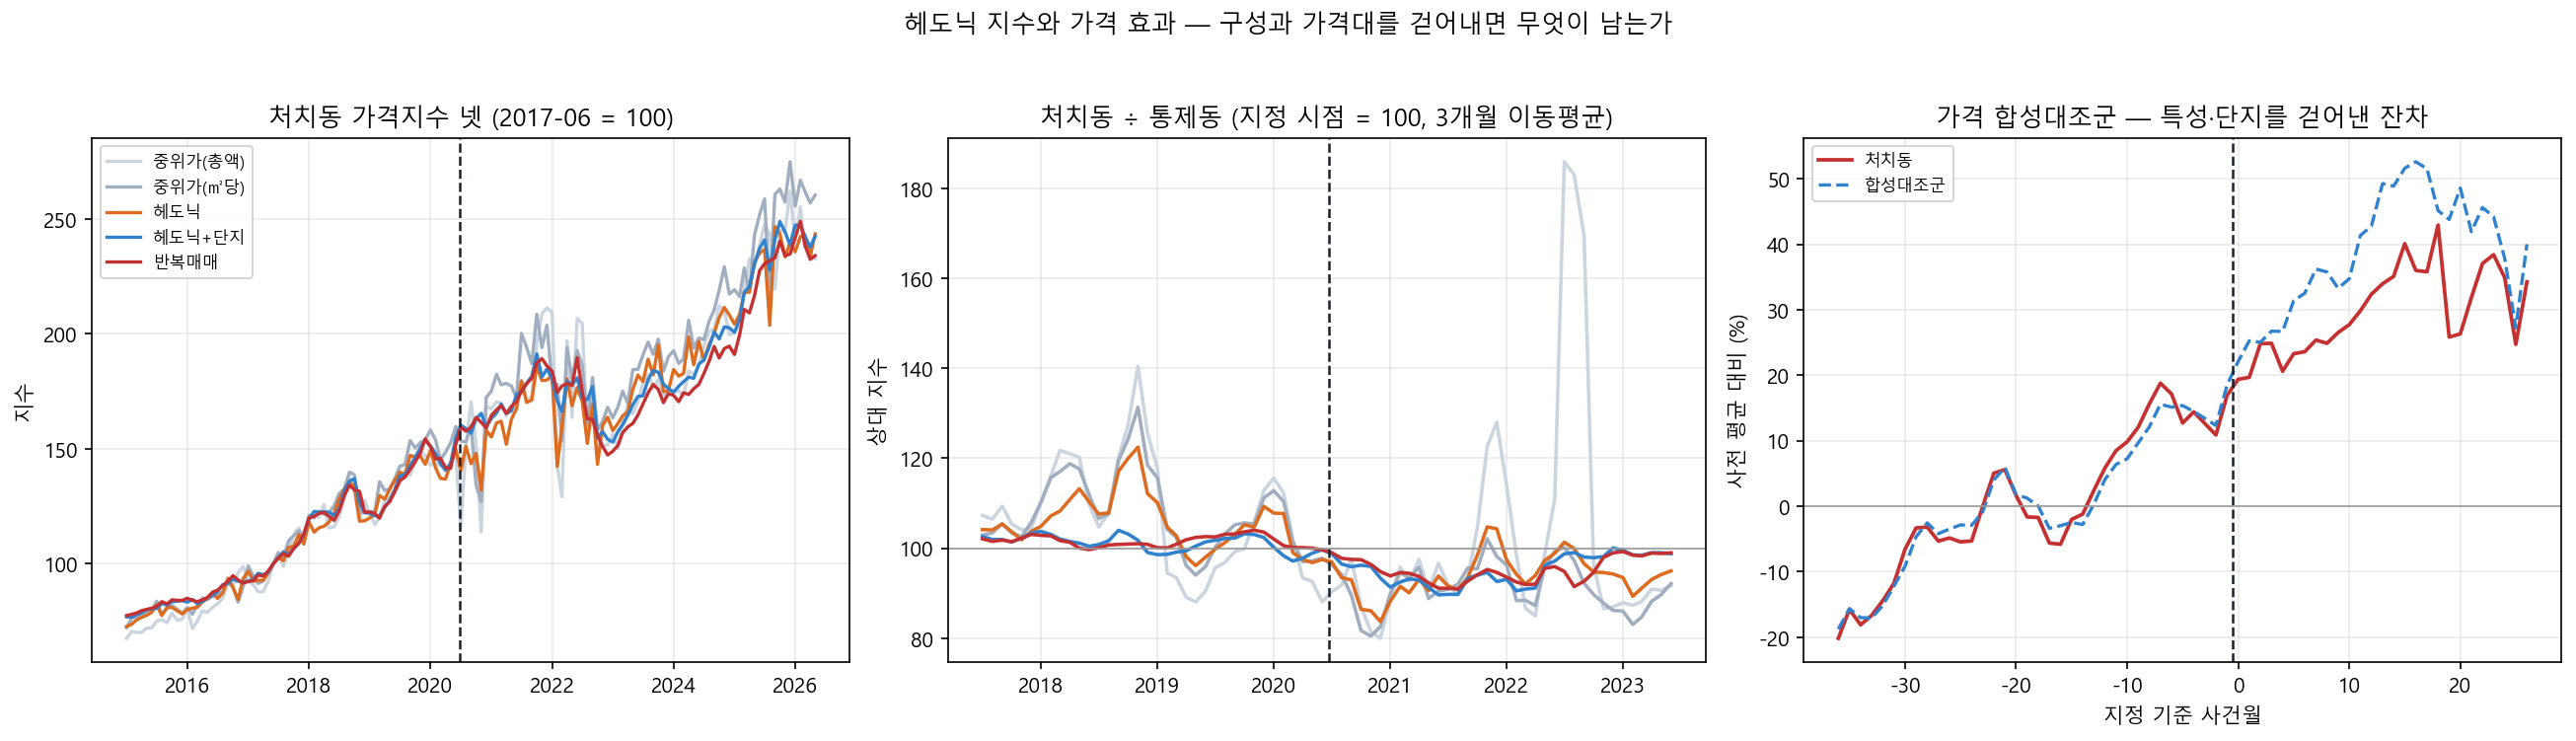
\includegraphics[width=\linewidth]{08_hedonic.png}
  \caption{가격지수 다섯과 통제군 격자.}
  \label{fig:hedonic}
\end{figure}

\textbf{결정적인 칸은 단지 고정효과다.} 면적·층만 통제하면 $-11.1\%$인데 어느
단지의 집이 팔렸는지까지 고정하면 $-5.9\%$로 절반이 된다. \textbf{집계 지수의
$-10 \sim -12\%$는 절반쯤이 구성 변화였다.}

그리고 \textbf{약점이 정반대인 두 방법이 $-5.9\%$와 $-6.0\%$에서 만난다.}
반복매매는 두 번 팔린 집만 쓰고(선택편의), 헤도닉은 모든 거래를 쓰되 관측되는
특성만 통제한다. 둘이 일치하면 서로를 떠받친다.

\subsection{통제군 격자}

통제군을 바꾸면 값이 흔들린다. 같은 창, 같은 지수로 통제군 둘 $\times$ 사양 넷을
돌렸다.

\begin{table}[htbp]
  \centering
  \caption{통제군을 바꿀 때 (12개월 변화)}
  \label{tab:price-grid}
  \begin{tabular}{lrrrr}
    \toprule
    \textbf{통제군} & \textbf{중위 총액} & \textbf{중위 ㎡당} &
    \textbf{헤도닉} & \textbf{헤도닉+단지} \\
    \midrule
    강남·송파 통제동 & $-5.5\%$ & $-6.7\%$ & $-4.2\%$ & $-5.9\%$ \\
    서울 나머지 19개 구 & $-9.8\%$ & $-10.7\%$ & $\mathbf{-2.1\%}$ &
      $-4.2\%$ \\
    \bottomrule
  \end{tabular}
\end{table}

처치동 아파트는 서울 최상위 가격대에 몰려 있고 2020$\sim$2021년은 중저가가
급등하고 고가가 뒤처진 시기다. 그래서 지정 전 ㎡당가가 처치동 범위에 드는 단지만
남긴 \textbf{공통지지} 표본에서는 가격 효과가 $-2.1\%$($p=0.270$)로 약해진다.

\textbf{읽는 방법이 둘이다.} 토허제의 가격 효과로 보였던 것이 사실은 2020$\sim$21년
고가 단지가 뒤처진 것일 수 있고, 반대로 규제가 고가 단지에 걸렸으니 가격대를
맞추는 것은 처치의 일부를 빼는 것일 수 있다. \textbf{지금 자료로는 가르지 못한다.}

\textbf{버린 사양을 밝혀 둔다.} 가격대를 통제하려고 처음에는 가격 10분위 $\times$
시점 고정효과를 넣었다. 처치동 가격 효과가 $-1.0\%$까지 사라지길래 확인해 보니
\textbf{최상위 분위 거래의 20.3\%가 처치동이고, 처치동과 맞닿은 동을 합치면
49.4\%}였다. 처치가 제 통제군이 되어 효과를 기계적으로 흡수하는 구조다. 고정효과로
빼는 대신 표본을 줄여 비교 대상을 명시적으로 고르는 쪽으로 바꿨다.

\subsection{사전 추세를 열면 무너진다}

지금까지 사전 추세는 \textbf{진단}만 했다(4.5절). 기준 분기를 옮겨 보는 것은 대안
사양 몇 개를 보는 것이지 \textbf{위배의 크기를 모수로 놓고 푸는 것이 아니다.}

\citet{rambachan2023honest}는 평행추세를 성립/불성립으로 묻지 않는다. 사후에 남아
있을 수 있는 위배를 모수 $\bar{M}$ 하나로 제한하고, 그 모수를 키워 가며
\textbf{구간이 언제 0을 품는지}를 본다. 그 지점이 \textbf{붕괴값}이다.
$\bar{M}=1$은 ``사전에 가장 크게 흔들렸던 만큼이 사후에도 매 분기 그대로
이어졌다''는 뜻이다.

\begin{table}[htbp]
  \centering
  \caption{사전 추세를 열어 둘 때의 붕괴값}
  \label{tab:breakdown}
  \begin{tabular}{lr}
    \toprule
    \textbf{무엇을 재나} & \textbf{붕괴값 $\bar{M}$} \\
    \midrule
    \textbf{거래량 --- 지정 직후 3개월} & $\mathbf{1.62}$ \\
    거래량 --- 24개월 평균 & 0.05 \\
    \textbf{가격 --- 지정 후 12개월} & $\mathbf{0.22}$ \\
    \bottomrule
  \end{tabular}
\end{table}

\begin{figure}[htbp]
  \centering
  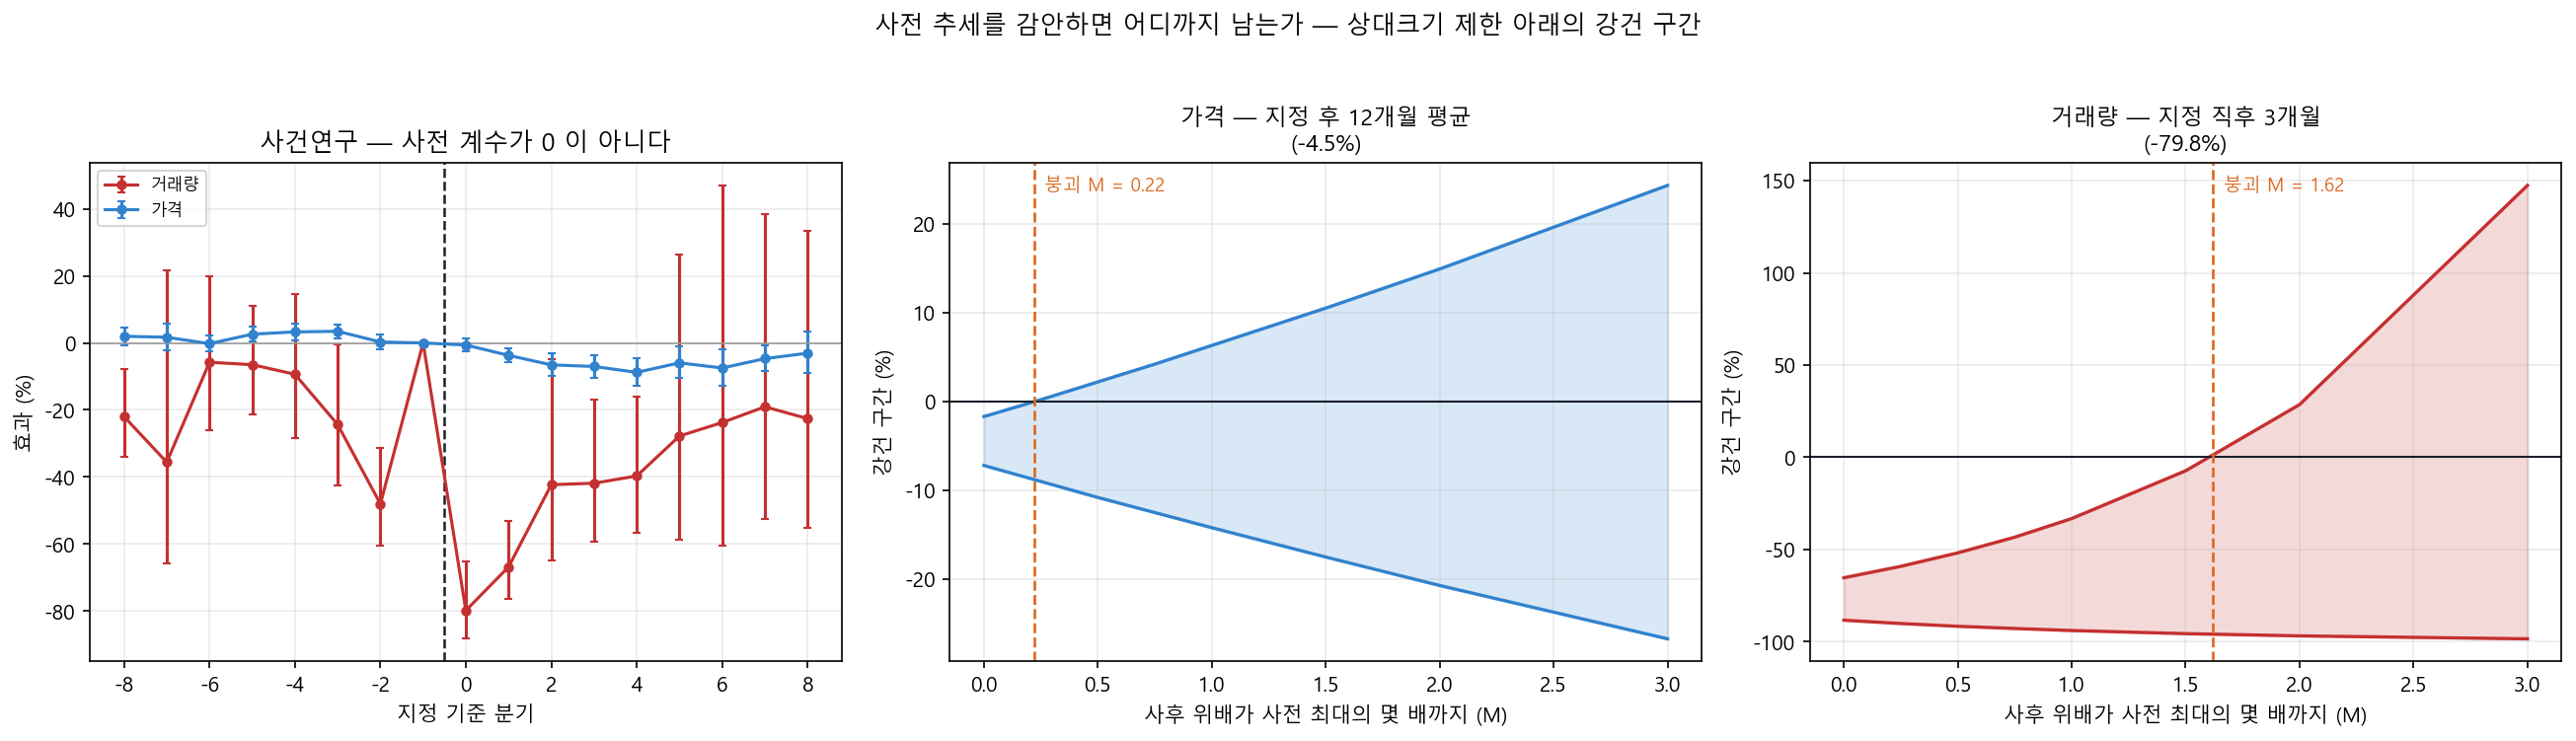
\includegraphics[width=\linewidth]{11_honest_did.png}
  \caption{사전추세 민감도 구간. $\bar{M}$ 을 키워 가며 구간이 0 을 품는 지점을
           본다.}
  \label{fig:honest-did}
\end{figure}

\textbf{거래량 직후 효과는 사전 위배의 1.6배까지 열어 두어도 남고, 가격은 0.22에서
무너진다.} 7분의 1이다. 가격 $-4 \sim -7\%$는 \textbf{평행추세를 가정했을 때만}
성립하는 값이다.

\subsection{합성대조군으로는 확인되지 않는다}

사람이 통제군을 고르지 않고 \textbf{사전 궤적이 가장 닮도록 자료가 가중치를 직접
찾게} 했다\citep{abadie2010synthetic}. 기증자 풀에서 맞닿은 동 14개는 뺀다 ---
7장에서 그 동들의 가격이 19개 구 대비 $-5.0\%$ 움직였으므로 파급을 받은 동을
통제군에 넣으면 효과가 0 쪽으로 끌린다(실제로 빼기 전 $-3.5\%$, 빼고 나서
$-5.1\%$).

\begin{table}[htbp]
  \centering
  \caption{합성대조군 --- 거래량과 가격}
  \label{tab:scm-compare}
  \begin{tabular}{llrr}
    \toprule
    \textbf{결과변수} & \textbf{검정 통계량} & \textbf{순위} &
    \textbf{경험적 $p$} \\
    \midrule
    거래량 & 지정 직후 3개월 ($-71.0\%$) & \textbf{1 / 152} &
      $\mathbf{0.007}$ \\
    거래량 & 사후 27개월 평균 ($-26.9\%$) & 22 / 152 & 0.145 \\
    가격 & 사후 12개월 평균 ($-5.1\%$) & 중간 & \textbf{0.511} \\
    \bottomrule
  \end{tabular}
\end{table}

\textbf{가격은 가짜 대치동 46개 가운데 중간쯤이다.} 우연과 구별되지 않는다.

\subsection{그래서 방향만 쓴다}

세 가지가 같은 방향을 가리킨다.

\begin{table}[htbp]
  \centering
  \caption{거래량과 가격 --- 같은 자료, 같은 사건, 같은 설계}
  \label{tab:vol-vs-price}
  \begin{tabular}{lrr}
    \toprule
    \textbf{검정} & \textbf{거래량} & \textbf{가격} \\
    \midrule
    설계 조합 중 유의하게 음수 & \textbf{192 / 192} & 70 / 144 \\
    붕괴값 $\bar{M}$ & \textbf{1.62} & 0.22 \\
    합성대조군 경험적 $p$ & \textbf{0.007} & 0.511 \\
    \bottomrule
  \end{tabular}
\end{table}

\textbf{그래서 가격은 ``내렸을 것이다''까지만 쓰고 ``몇 \% 내렸다''는 쓰지 않는다.}
설계를 바꿔 가며 144가지로 재면 $-18.2\%$에서 $+3.6\%$까지 움직이고 29개는 0 위로
올라간다. 거래량은 192가지 중 하나도 0을 넘지 않는다.

1주차에 주 결과변수를 가격에서 거래량으로 바꾼 것은 그때는 판단이었다(0001).
\textbf{다섯 달 뒤 세 가지 방법으로 그 결정이 확인됐다.}

\textbf{마지막으로 가격을 버리지 않은 이유를 적는다.} 선행연구 세 편이 모두 가격을
다루므로, 가격을 빼면 대조할 지점이 사라진다. 그리고 ``가격을 잡았다는 증거가
약하다''는 것 자체가 제도 평가의 결과다. 명분이 가격 안정인 제도에서 그 명분이
확인되지 않는다는 것은 \textbf{못 잰 것이 아니라 재서 알게 된 것}이다.

% 9장 강건성. 0016 · 0017 · 0020 · 0027 · 0028 · 0030 · 0031

\section{강건성}

이 장은 \textbf{결과를 무너뜨리려는 시도}를 모은 것이다. 일곱 가지를 걸었고, 그중
둘은 ``걸어 봤더니 가릴 수 없다''가 결과였다. 그것도 적는다.

\subsection{위약 검정}

위약 검정은 효과를 재는 것이 아니라 \textbf{측정 도구를 검사}하는 것이다. 아무 일도
없었어야 할 자리에 같은 추정을 돌려 0이 나오는지 본다. 0이 나오지 않으면 그 설계가
\textbf{없는 효과도 만들어 낸다}는 뜻이다.

필요가 생긴 이유가 있다(0016). 고가 처치동은 처치 전에 이미 특이했다 --- 법정동
$\times$ 사건월 칸당 평균 42.2건으로 고가 통제동(15.7건)의 2.7배였고 사후에
10.3 대 8.7로 수렴한다. \textbf{`원래 활발하던 곳이 평균으로 돌아온 것'과 `규제가
거래를 막은 것'은 자료에서 같게 보인다.}

이 절의 숫자는 \textbf{사후 24개월을 하나로 묶은 이중차분}($-33.5\%$)이며, 5장의
직후 효과와 \textbf{다른 값}이다. 섞어 쓰면 안 된다.

% 자동 생성 — scripts/build_tables.py. 손으로 고치지 않는다.
% 출처: output/results/13_placebo.json : A_가짜사건일
\begin{table}[htbp]
  \centering
  \caption{위약 --- 지정이 없던 날을 사건일로 두고 같은 추정을 돌렸다.}
  \label{tab:placebo-date}
  \begin{tabular}{lrr}
    \toprule
    \textbf{가짜 사건일} & \textbf{효과 (\%)} & \textbf{$p$} \\
    \midrule
    2013-06-23 & -5.0 & 0.699 \\
    2014-06-23 & -4.3 & 0.663 \\
    2015-06-23 & -9.7 & 0.088 \\
    2016-06-23 & -21.5 & 0.021 \\
    2017-06-23 & -16.6 & 0.049 \\
    2023-06-23 & -2.3 & 0.836 \\
    2024-06-23 & -1.9 & 0.864 \\
    \bottomrule
  \end{tabular}

  \begin{minipage}{\linewidth}\footnotesize
  \textit{주.} 진짜($-33.5\%$)가 가짜 최대($-21.5\%$)의 1.5배다. 다만 2016·2017 창에는 8·2 와 9·13 대책이 들어 있어 완전한 위약이 아니다.
  \end{minipage}
\end{table}


\begin{figure}[htbp]
  \centering
  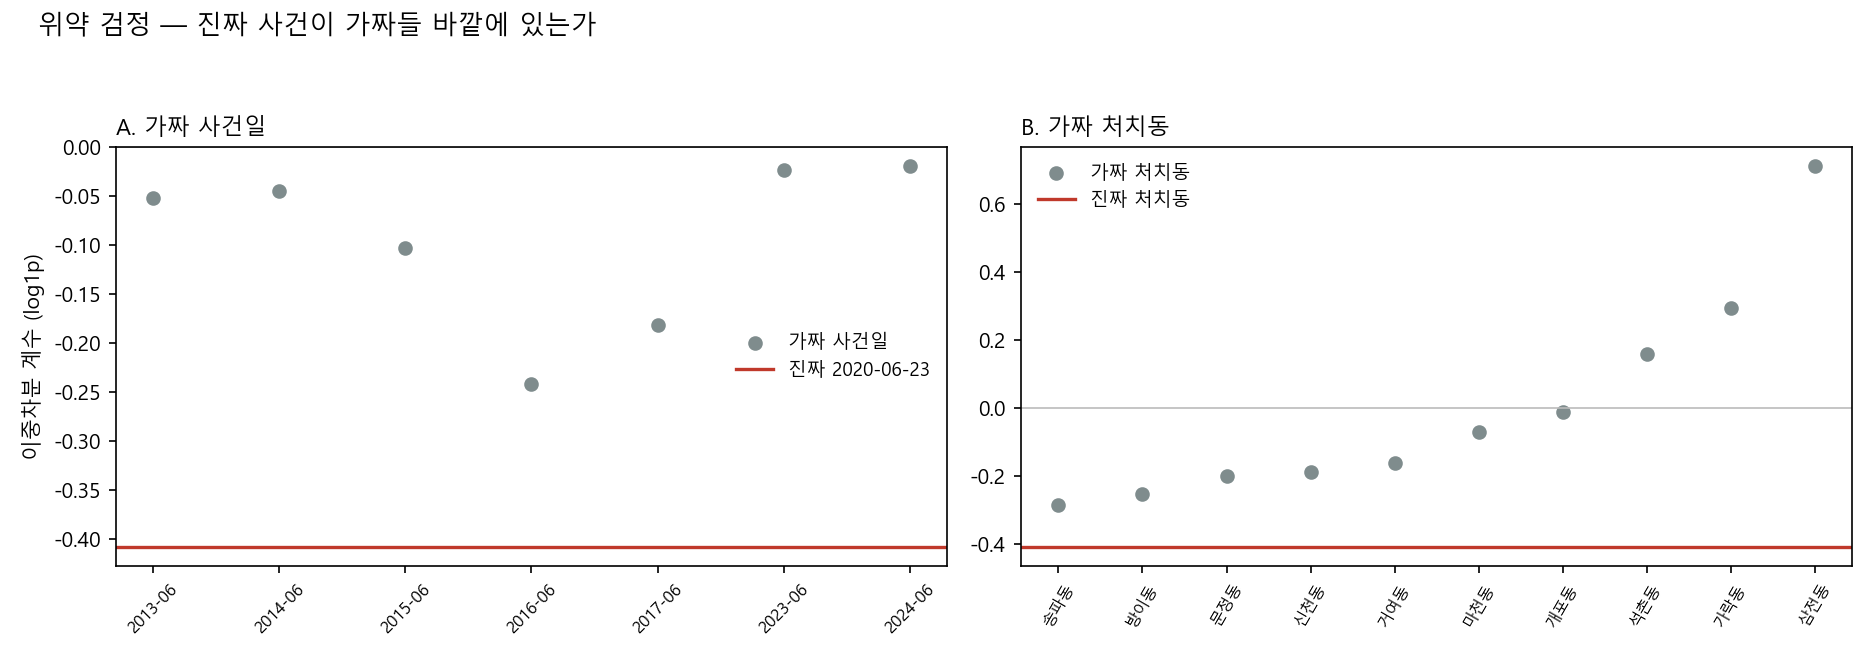
\includegraphics[width=\linewidth]{13_placebo.png}
  \caption{위약 검정. 왼쪽 가짜 사건일, 오른쪽 가짜 처치동.}
  \label{fig:placebo}
\end{figure}

\textbf{진짜가 가짜 최대($-21.5\%$)의 1.5배다. 그러나 가짜 둘이 유의하다.}
2016·2017년 창에는 \textbf{8·2 대책(2017-08)과 9·13 대책(2018-09)}이 들어 있고
둘 다 처치동에 더 크게 걸리는 규제다. \textbf{완전한 위약이 아니다.}

\textbf{가짜 처치동}으로도 돌렸다. 강남·송파 비처치동 23개 중 나중에 동 전체로
지정된 13개를 빼고 남은 10개를 처치군인 척 세우면 $-24.8\%$에서 $+103.5\%$까지
퍼지고, \textbf{진짜($-33.5\%$)가 그중 가장 크다.}

\textbf{그래서 0016의 결론은 ``효과는 있으나 크기는 구간으로 말한다''였다.}
24개월 효과를 단일 숫자로 쓰지 않는 이유의 하나다.

\subsection{합성대조군}

위약 검정이 숙제를 남겼다. 사전 거래량을 손으로 맞출수록 효과가 $-33.5\%$에서
$-24.8\%$로 줄고 유의성도 약해졌다 --- \textbf{평균 회귀가 섞였을 가능성을 배제하지
못했다.} 손으로 문턱을 정하는 방식은 문턱이 임의고, 표본을 버려 검정력도 잃으며,
사전 거래량으로 표본을 고르는 것 자체가 새로운 선택 편의를 만든다.

합성대조군은 \textbf{사전 궤적이 처치군과 가장 비슷해지도록 통제군의 가중평균을
자료가 직접 찾는다}\citep{abadie2010synthetic}. 문턱이 없고 표본을 버리지 않는다.

\begin{table}[htbp]
  \centering
  \caption{합성대조군 설계}
  \label{tab:scm-design}
  \begin{tabular}{ll}
    \toprule
    처치 단위 & 청담·삼성·대치·잠실을 합친 \textbf{하나} \\
    기증자 & 동 전체 지정 이력이 없고 사전 월평균 3건 이상인 서울 법정동
      \textbf{151개} \\
    결과변수 & $\log(1+\text{월 거래건수})$ $-$ 그 단위의 사전 36개월 평균 \\
    가중치 & 음수 아님, 합 1. 사전 36개월 궤적의 제곱오차 최소화 \\
    추론 & 배치 위약 --- 기증자 각각을 처치인 척 돌려 순위를 본다 \\
    \bottomrule
  \end{tabular}
\end{table}

\textbf{수준을 빼야 했다.} 처음에는 수준을 그대로 썼고 실패했다(사전 RMSPE 0.41,
경험적 $p$ 0.57). 처치 단위는 4개 동을 합쳐 월 210.9건인데 기증자 법정동은 중앙값
7.2건이다. \textbf{가중치가 음수가 아니고 합이 1이므로 볼록결합으로는 그 수준에
닿을 수 없다.} 단위별 사전 평균을 빼면 모두 0에서 출발해 궤적의 \emph{모양}만
맞추게 된다 --- 이중차분의 단위 고정효과와 같은 조작이다. 사전 RMSPE가 0.41에서
\textbf{0.17}로 떨어졌다.

\begin{figure}[htbp]
  \centering
  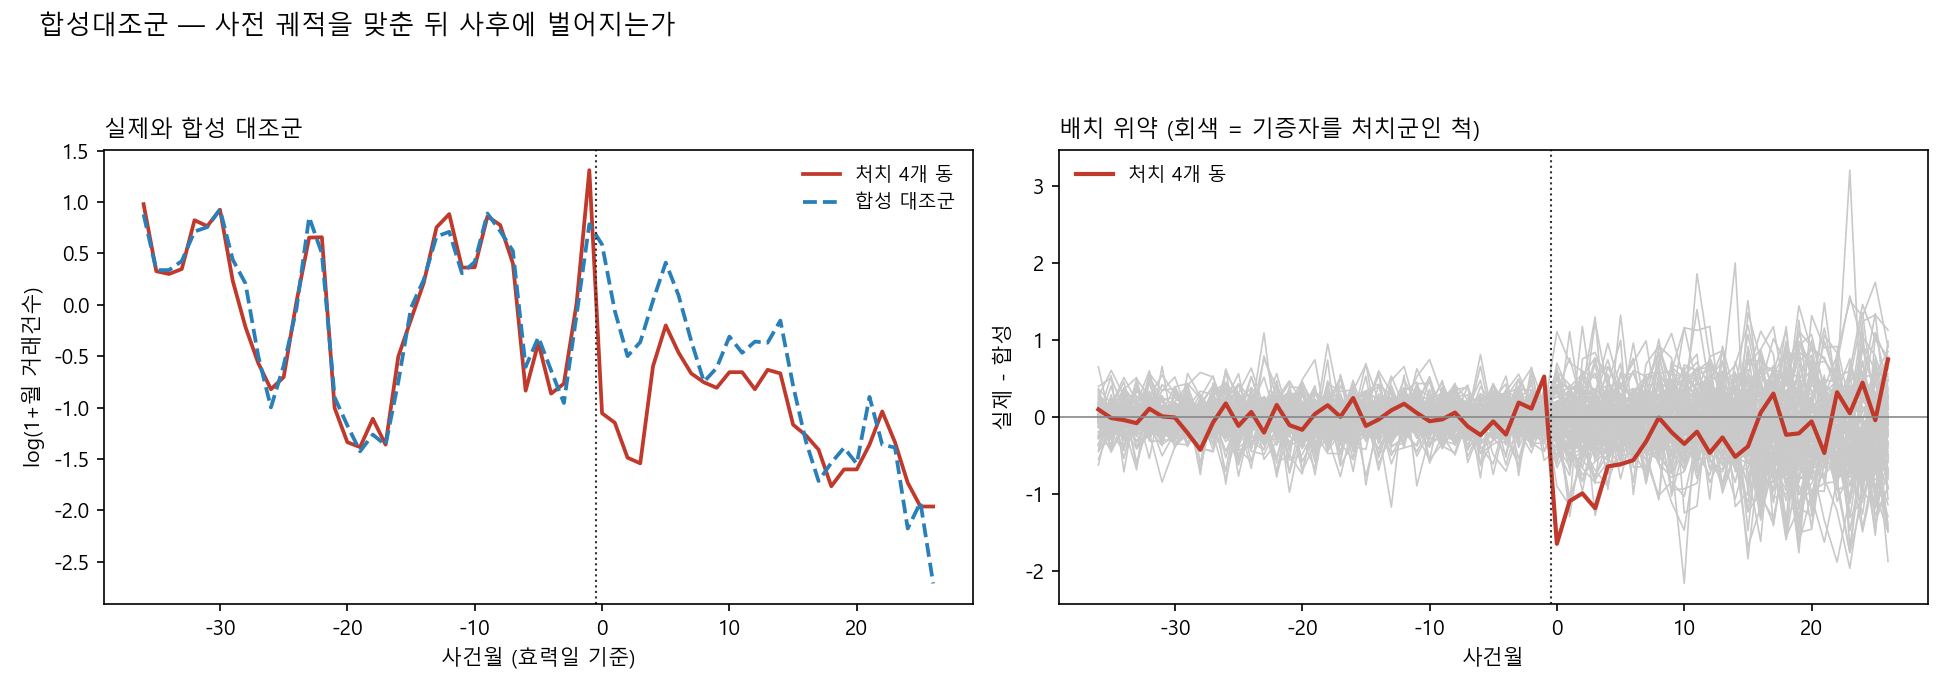
\includegraphics[width=\linewidth]{17_scm.png}
  \caption{합성대조군과 배치 위약. 빨간 선이 진짜 처치 단위, 회색이 기증자
           151개를 처치인 척 돌린 것이다.}
  \label{fig:scm}
\end{figure}

결과는 8.5절의 표~\ref{tab:scm-compare}에 있다. \textbf{지정 직후 3개월은 152개 중
1위($p=0.007$), 사후 27개월 평균은 22위($p=0.145$)다.} 사전 적합이 나쁜 가짜를
빼도(진짜의 2배 이내, 106개) 0.009와 0.206으로 같은 결론이다.

\textbf{통계량 선택의 순서를 밝힌다.} 사후 평균을 \emph{먼저} 돌렸고 유의하지
않았다. 그다음 직후 3개월로 바꾸어 유의한 값을 얻었다. 순서만 보면 사양 탐색이다.
다만 ``사후 $k \geq 4$는 해석하지 않는다''는 결정(0014)이 \textbf{이 분석보다 먼저}
있었고, 사후 27개월 평균은 그 해석하지 않기로 한 구간을 대부분 포함한다.
\textbf{둘 다 보고한다.}

\subsection{통제군 오염 제외}

강남·송파 통제동 23개 가운데 여섯이 분석 창 안에서 지정됐다(0009). 통제군이 일부
처치를 받으면 처치·통제 격차가 줄어 추정치가 0 쪽으로 끌린다(감쇠). 방향이
유리하다고 넘기지 않고 \textbf{이 동들을 뺀 사양을 함께 보고한다.}

\begin{table}[htbp]
  \centering
  \caption{창 안에 지정된 통제동 여섯}
  \label{tab:contam-list}
  \begin{tabular}{llrl}
    \toprule
    \textbf{동} & \textbf{지정 시작} & \textbf{사건월} & \textbf{방식} \\
    \midrule
    거여동 & 2021-04-04 & 9 & 혼합 \\
    압구정동 & 2021-04-27 & 10 & \textbf{동 전체} \\
    마천동 & 2022-01-02 & 18 & 혼합 \\
    송파동 & 2022-01-29 & 19 & 혼합 \\
    신천동 & 2022-01-29 & 19 & 혼합 \\
    일원동 & 2022-01-29 & 19 & 일부 \\
    \bottomrule
  \end{tabular}
\end{table}

\textbf{가장 이른 오염이 사건월 9다.} 지정 직후 3개월(사건월 0$\sim$2)에는 통제군
오염이 하나도 없다. 그러므로 직후 효과는 오염으로 줄어들 수 없다.

% 자동 생성 — scripts/build_tables.py. 손으로 고치지 않는다.
% 출처: output/results/13b_contamination.json : 결과
\begin{table}[htbp]
  \centering
  \caption{통제군 오염 동을 빼도 지정 직후 효과는 그대로다.}
  \label{tab:contamination}
  \begin{tabular}{lrrrr}
    \toprule
    \textbf{표본} & \textbf{법정동} & \textbf{효과 (\%)} & \textbf{WCR $p$} & \textbf{무작위화 순위} \\
    \midrule
    기본 & 27 & -79.8 & 0.014 & 1 \\
    압구정 제외 & 26 & -80.0 & 0.013 & 1 \\
    오염 6개 제외 & 21 & -80.0 & 0.008 & 1 \\
    \bottomrule
  \end{tabular}

  \begin{minipage}{\linewidth}\footnotesize
  \textit{주.} 가장 이른 오염이 사건월 9 다. 지정 직후 3개월에는 오염이 없다. 제외 목록은 결과를 보기 전(2026-09-07)에 정했다.
  \end{minipage}
\end{table}


\begin{figure}[htbp]
  \centering
  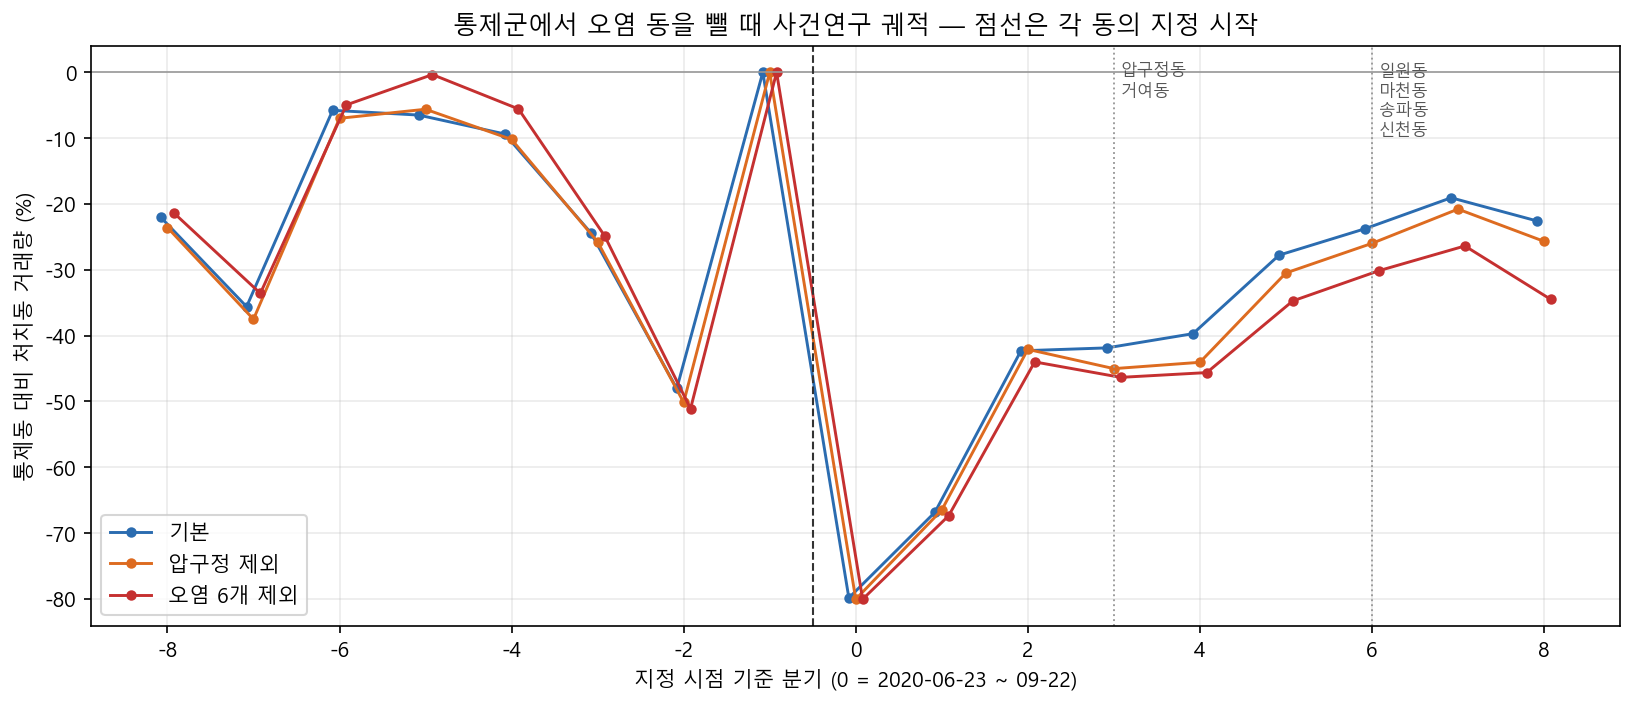
\includegraphics[width=\linewidth]{13b_contamination.png}
  \caption{오염 동을 뺄 때의 사건연구 궤적.}
  \label{fig:contamination}
\end{figure}

\textbf{직후 효과는 움직이지 않고($-79.8 \to -80.0\%$) 24개월 효과는 커진다}
($-33.5 \to -38.4\%$, WCR $p$ $0.047 \to 0.015$). 5.4절에서 ``24개월은 경계에
있다''고 적은 그 경계의 일부가 오염에 의한 감쇠였다. 모든 표본에서 무작위화
\textbf{1위}다.

\textbf{제외 목록은 결과를 보기 전에 정했다.} 0009가 2026-09-07에 목록을
확정했고 이 분석은 09-18에 했다. 결과를 보고 고른 표본이 아니다.

\subsection{처치 역전 --- 가중치와 $\text{DID}_M$}

제안서는 2025년 처치 역전 구간에 \citet{dechaisemartin2020twoway}의 비흡수 처치
추정량을 쓰겠다고 적었다. 그 약속의 이행이다(0027).

양방향 고정효과 추정량은 처치 효과가 이질적일 때 일부 칸에 \textbf{음의 가중치}를
줄 수 있다\citep{goodmanbacon2021}. 이미 처치된 집단이 다른 집단의 통제군 노릇을
하기 때문이다.

\textbf{표준적인 이질적 처치시점 추정량을 쓸 수 없는 이유를 먼저 적는다.}
\citet{callaway2021}와 \citet{sunabraham2021}은 처치가 한 번 시작되면
유지된다는 \textbf{흡수(absorbing) 가정}에 의존한다. 2025년 구간에서 A그룹의
처치 상태는 $1 \to 0 \to 1$로 전환되므로 그대로 적용할 수 없다. 그래서
비흡수 처치를 다루는 \citet{dechaisemartin2020twoway}의 $\text{DID}_M$을 쓴다.
합성 이중차분\citep{arkhangelsky2021}도 후보였으나, 처치 단위가 하나(4개 동을
합친 것)이고 역전 구간이 39일로 짧아 사전 적합에 쓸 구간이 부족해 쓰지 않았다.

\begin{table}[htbp]
  \centering
  \caption{TWFE 가중치 진단}
  \label{tab:dcdh-weights}
  \begin{tabular}{lrrr}
    \toprule
    \textbf{패널} & \textbf{처치 칸} & \textbf{음의 가중치} &
    \textbf{음의 가중치 합} \\
    \midrule
    \textbf{2020 주 분석} & 108 & \textbf{0개} & 0.000 \\
    2025 해제·재지정 & 5{,}350 & 675개 (12.6\%) & $-0.023$ \\
    \bottomrule
  \end{tabular}
\end{table}

\textbf{주 분석 패널에는 음의 가중치가 하나도 없다.} 2025 구간에도 합이 $-0.023$로
작다. $\text{DID}_M$으로 다시 재면 부과(재지정)가 $-43.0\%$
$[-50.8, -33.3]$, 해제가 $-28.2\%$ $[-58.9, +11.7]$이고 위약은 $+1.9\%$,
$-2.7\%$로 깨끗하다.

\begin{figure}[htbp]
  \centering
  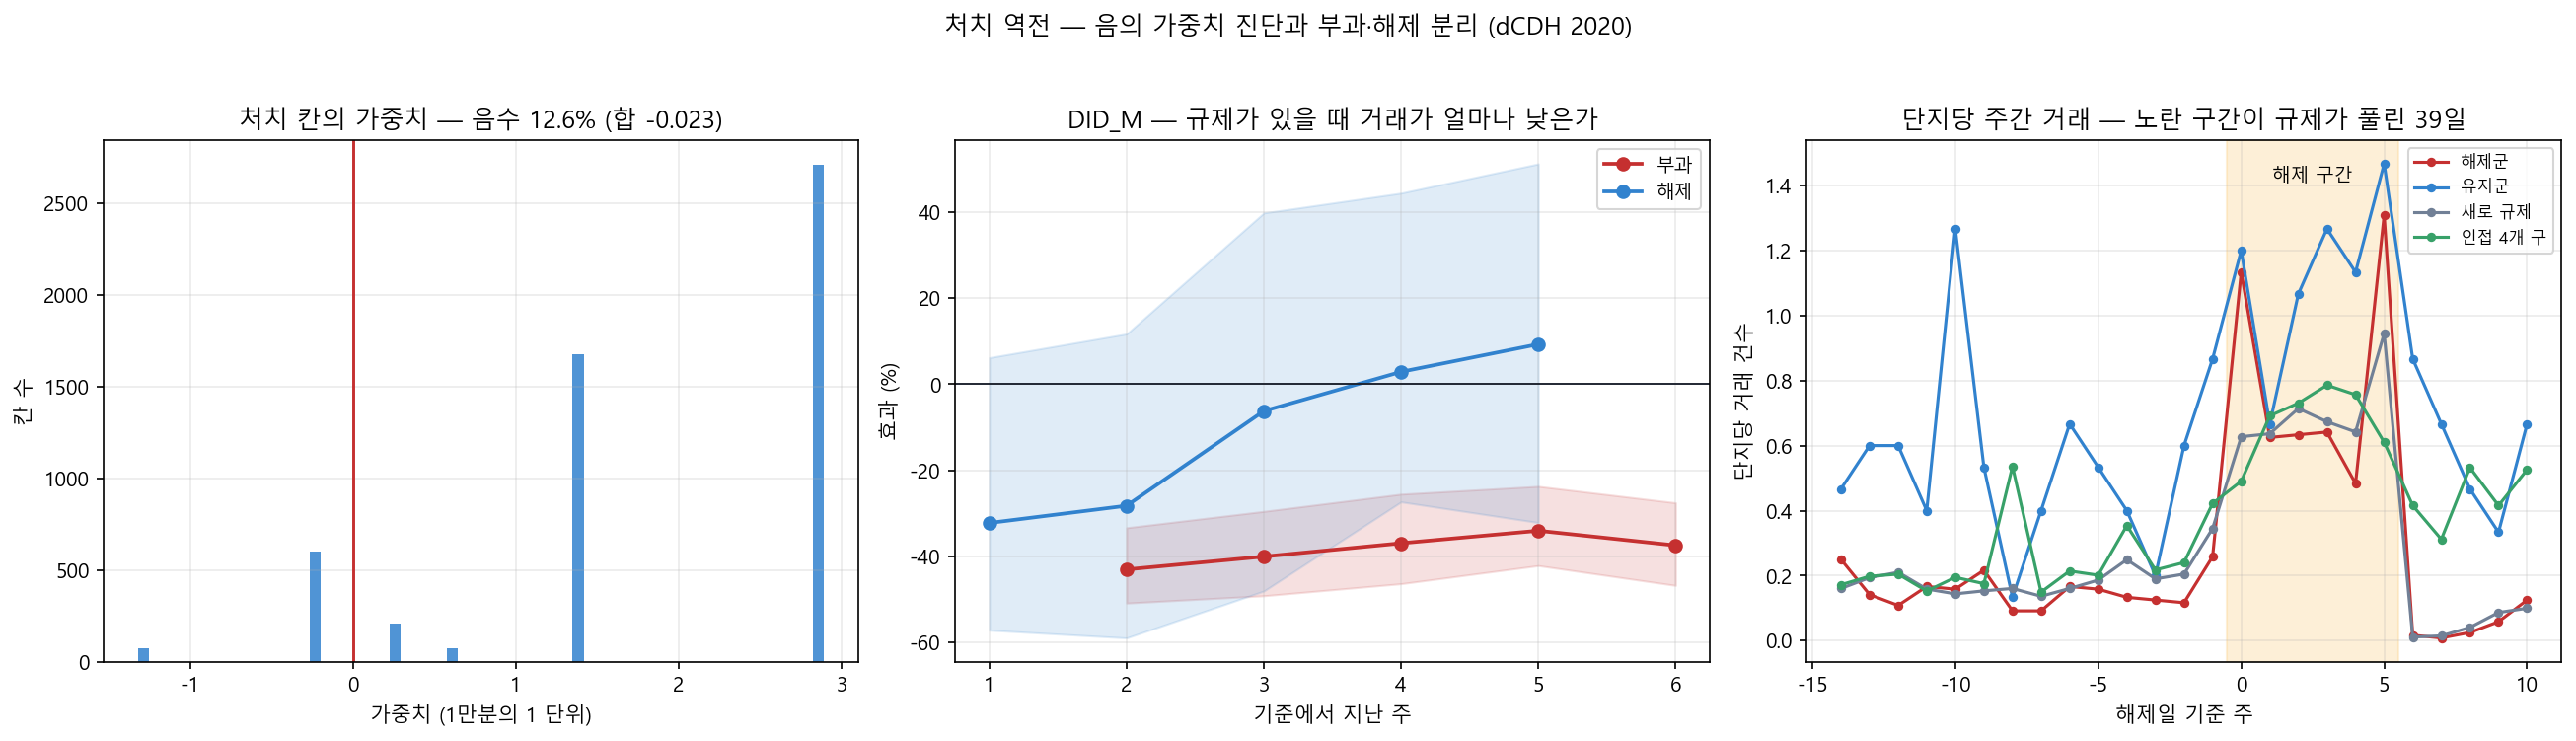
\includegraphics[width=\linewidth]{10_dcdh.png}
  \caption{TWFE 가중치 분포와 $\text{DID}_M$.}
  \label{fig:dcdh}
\end{figure}

\textbf{결론은 ``바꿀 필요가 없다''이다.} 그리고 \textbf{대칭성은 가릴 수 없다} ---
부과 쪽은 구간이 0을 품지 않고 해제 쪽은 품는다. 처음에는 ``처음 두 주만
대칭''이라고 썼다가, 막차 주간을 뺀 탓에 부과의 lag 0이 2주 변화였던 것을 발견해
\textbf{경과 주를 맞춰 다시 쟀다.} 결론이 바뀌었다.

\textbf{안 해 봤으면 몰랐다는 점이 결과다.}

\subsection{사양 곡선}

합리적인 설계 선택을 전부 조합했다(2.4절, 0028). 축과 조합 수는 그 절에 있다.

\begin{table}[htbp]
  \centering
  \caption{사양 곡선 요약}
  \label{tab:spec-summary}
  \begin{tabular}{lrr}
    \toprule
    & \textbf{거래량} & \textbf{가격} \\
    \midrule
    사양 수 & 192 & 144 \\
    중위 & $-68.9\%$ & $-5.3\%$ \\
    범위 & $-86.4 \sim -21.2\%$ & $-18.2 \sim \mathbf{+3.6\%}$ \\
    음수 & \textbf{100.0\%} & 79.9\% \\
    유의하게 음수 & \textbf{100.0\%} & \textbf{48.6\%} \\
    \bottomrule
  \end{tabular}
\end{table}

\begin{figure}[htbp]
  \centering
  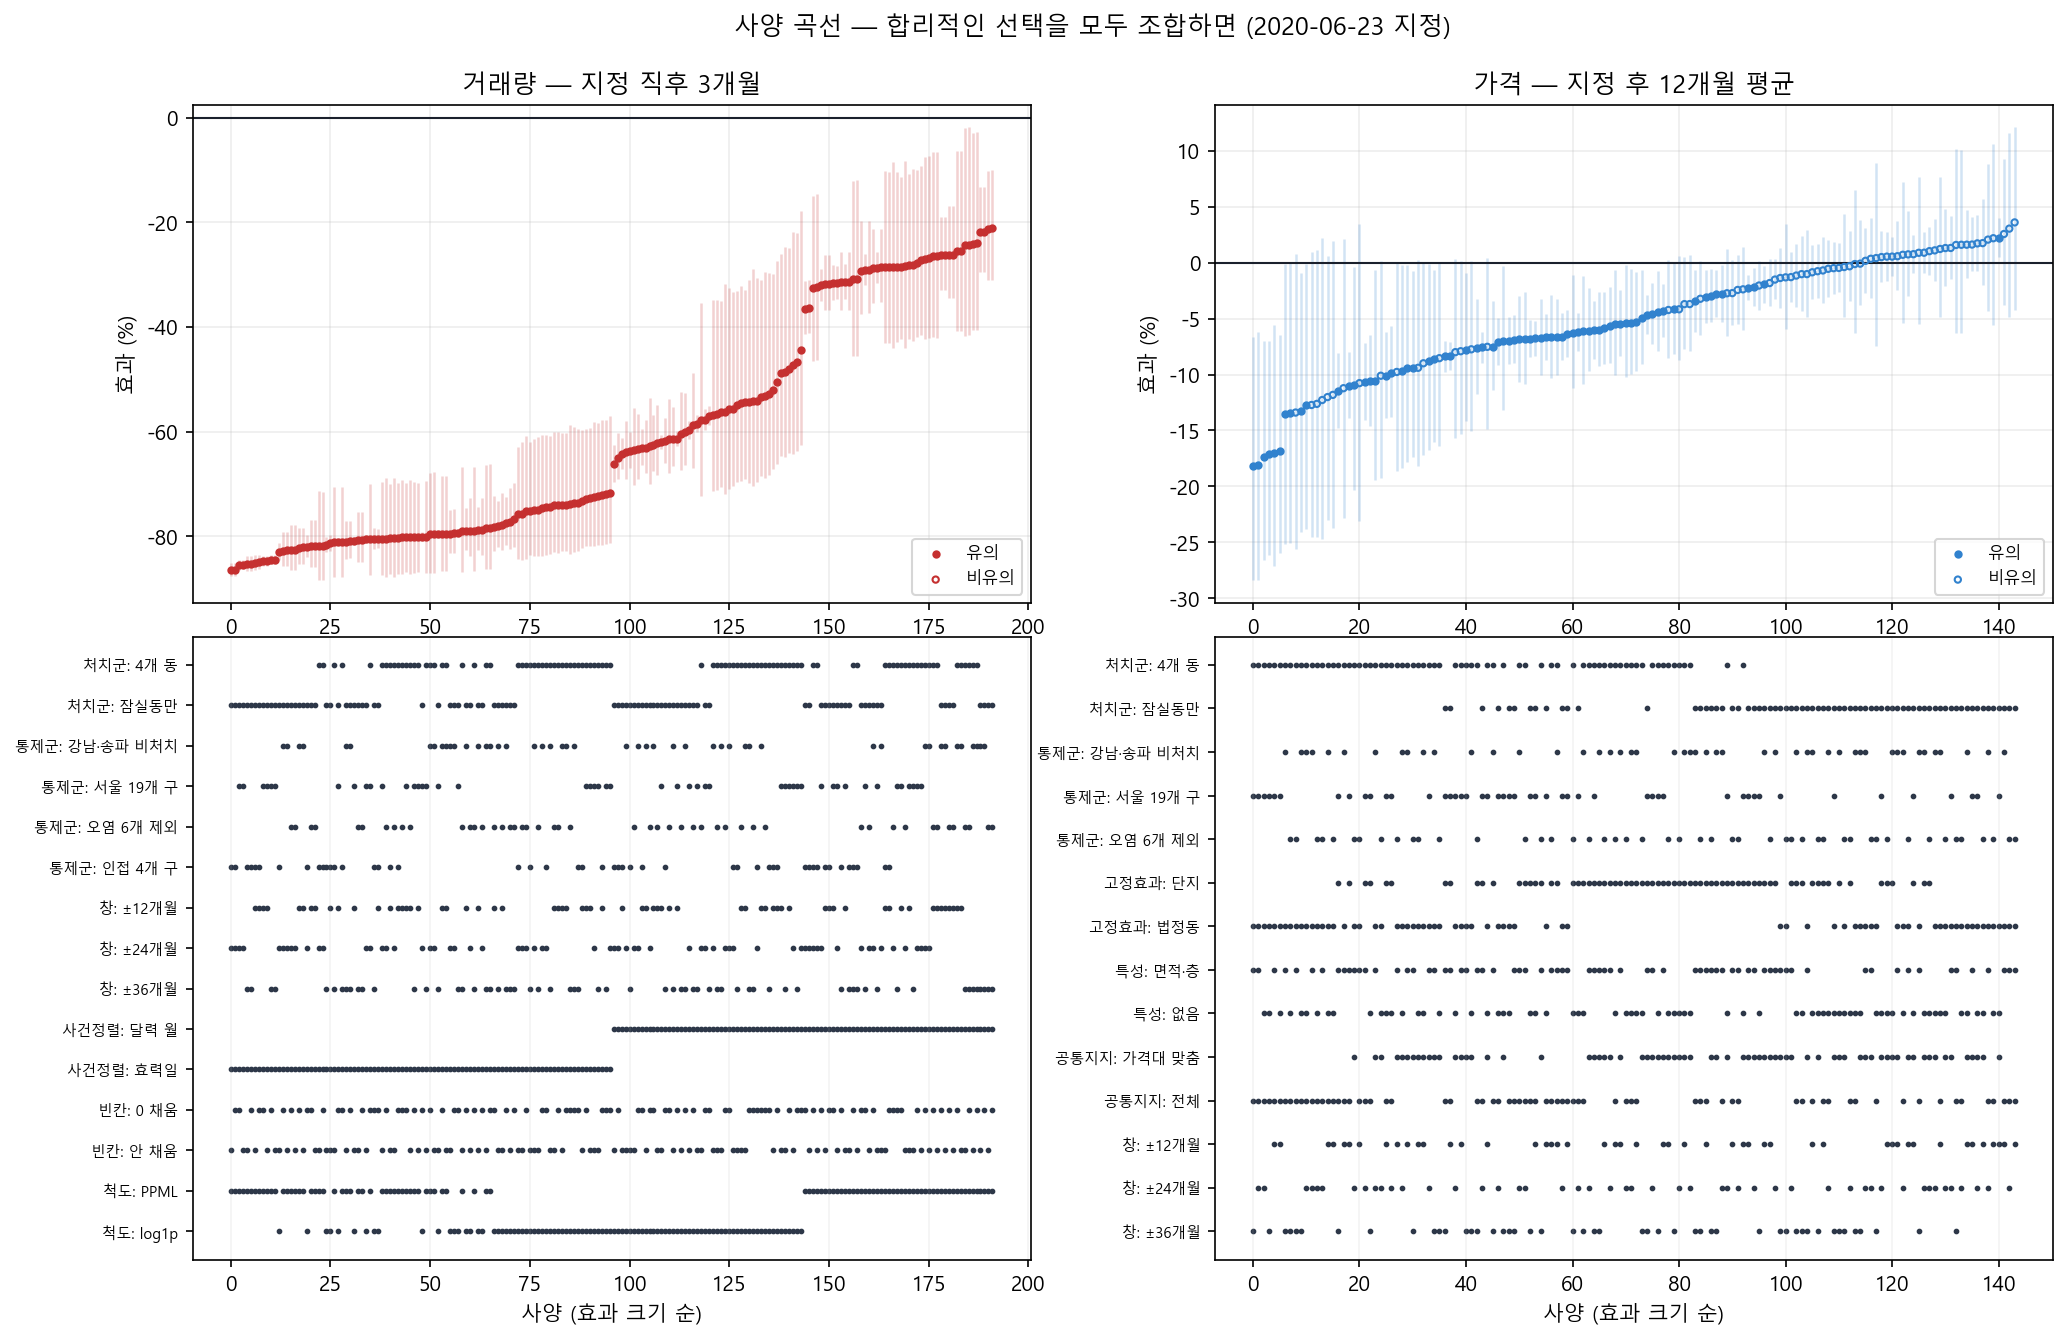
\includegraphics[width=\linewidth]{05b_spec_curve.png}
  \caption{사양 곡선. 점 하나가 설계 조합 하나로 추정한 효과이고, 아래 칸은 그
           조합이 어떤 선택을 썼는지다. 왼쪽 거래량 192, 오른쪽 가격 144.}
  \label{fig:spec-curve}
\end{figure}

\textbf{거래량은 192개가 전부 0 아래다.} 처치군을 잠실동 하나로 줄이든, 통제군을
서울 19개 구로 넓히든, 창을 $\pm$12에서 $\pm$36으로 늘리든, 달력 월로 세든, 빈칸을
안 채우든, 척도를 바꾸든 마찬가지다.

\textbf{다만 방향이 안 갈린다는 것은 당연한 쪽이다.} 거래에 허가를 붙였으니
줄어든다. \textbf{갈리는 것은 크기이고}($-21\%$에서 $-86\%$까지), 그래서 ``무엇이
그 차이를 만들었나''가 다음 질문이 되며 그 답이 2.4절의 축별 분해다.

\textbf{표준오차에 단서를 단다.} 사양 곡선의 $p$는 법정동 군집 관행값이다. 처치
동이 적은 사양에서는 이 $p$가 너무 작다(5.3절). \textbf{곡선은 점추정을 보는
그림이고 구간은 참고로만 읽는다.} ``192개 전부 유의''는 그래서 과대평가이고, 믿을
것은 \textbf{192개 전부 음수}라는 쪽이다.

\subsection{외적 타당성 --- 2021년 B그룹}

처치 동이 네 개뿐이다. 17,550가지 중 1위는 \textbf{``그 네 동이 우연이 아니다''일
뿐 ``다른 동에서도 그렇다''가 아니다.} 둘은 다른 주장이다.

2021년 4월 27일 지정된 B그룹(압구정·여의도·목동·성수동1가·2가)을 두 번째 사례로
걸었다(0031). \textbf{완전히 다른 네 자치구}(강남·영등포·양천·성동), 열 달 뒤의
사건이다.

\textbf{설계의 핵심은 대칭이다.} B그룹 숫자를 A그룹 숫자 옆에 그냥 놓으면 안 된다.
A는 같은 구 안(강남·송파)을 통제군으로 썼는데 B는 그럴 수 없다 --- 목동이 속한
\textbf{양천구에 쓸 수 있는 비지정 동이 0개}다. 차이가 지역 때문인지 통제군
때문인지 가릴 수 없게 된다. 그래서 둘을 했다.

\begin{enumerate}[leftmargin=2em, itemsep=2pt]
  \item \textbf{두 사건을 같은 통제군 정의(서울 전역 비지정)로 다시 잰다.}
        A의 주 사양($-79.8\%$)은 그대로 두고 이 재추정은 비교용이다.
  \item \textbf{두 패널을 쌓아 차이를 직접 추정한다}(stacked DID). 두 숫자를
        눈으로 견주면 `차이가 유의한가'를 말할 수 없다 --- 6.3절에서 같은 실수를
        하고 정정했다.
\end{enumerate}

통제군에서 창 안에 어떤 계열로든 지정된 동 77개, A그룹 처치동 4개와 맞닿은 동
14개, 상대 사건의 처치동, 창 안 거래 30건 미만을 뺐다. \textbf{B그룹 5개 동 중
3개(압구정·성수동1가·2가)가 A그룹 맞닿은 동}이므로 처치군을 둘로 나눠 돌렸다.

% 자동 생성 — scripts/build_tables.py. 손으로 고치지 않는다.
% 출처: output/results/21_b_group.json : 대칭
\begin{table}[htbp]
  \centering
  \caption{두 사건을 같은 자로. 같은 통제군 정의, 같은 창, 같은 추정량.}
  \label{tab:bgroup}
  \begin{tabular}{lrrrr}
    \toprule
    \textbf{사양} & \textbf{처치 동} & \textbf{효과 (\%)} & \textbf{WCR $p$} & \textbf{무작위화 $p$} \\
    \midrule
    A 2020.6 (처치 4개 동) & 4 & -49.2 & 0.038 & $<0.001$ \\
    B 2021.4 (처치 5개 동) & 5 & -44.7 & 0.057 & $<0.001$ \\
    B 2021.4 (목동·여의도만) & 2 & -46.2 & 0.136 & 0.001 \\
    \bottomrule
  \end{tabular}

  \begin{minipage}{\linewidth}\footnotesize
  \textit{주.} 창 전체($\pm$12개월) 이중차분이다. 늘 인용하는 $-79.8\%$ 는 지정 직후 3개월이라 재는 것이 다르다. 두 사건의 차이를 쌓아서 직접 추정하면 $+8.7\%$, 무작위화 $p=0.715$ 다.
  \end{minipage}
\end{table}


% 자동 생성 — scripts/build_tables.py. 손으로 고치지 않는다.
% 출처: output/results/21_b_group.json : 사다리
\begin{table}[htbp]
  \centering
  \caption{2021.4 B그룹 --- 기준점을 바꿔도 $-41.7 \sim -44.9\%$ 다.}
  \label{tab:ladder-b}
  \begin{tabular}{lrrrr}
    \toprule
    \textbf{기준점} & \textbf{동} & \textbf{효과 (\%)} & \textbf{WCR $p$} & \textbf{무작위화 $p$} \\
    \midrule
    ① 서울 전역 비지정 & 182 & -44.7 & 0.057 & $<0.001$ \\
    ② ① + 가격대 공통지지 & 39 & -41.7 & 0.063 & 0.002 \\
    ③ 오염 미제외 & 233 & -43.8 & 0.071 & $<0.001$ \\
    ④ A그룹 맞닿은 동 포함 & 188 & -44.9 & 0.063 & $<0.001$ \\
    \bottomrule
  \end{tabular}

  \begin{minipage}{\linewidth}\footnotesize
  \textit{주.} 목동이 속한 양천구에 쓸 수 있는 비지정 동이 0개라 `같은 구 안' 통제군을 주 사양으로 쓸 수 없었다.
  \end{minipage}
\end{table}


\begin{figure}[htbp]
  \centering
  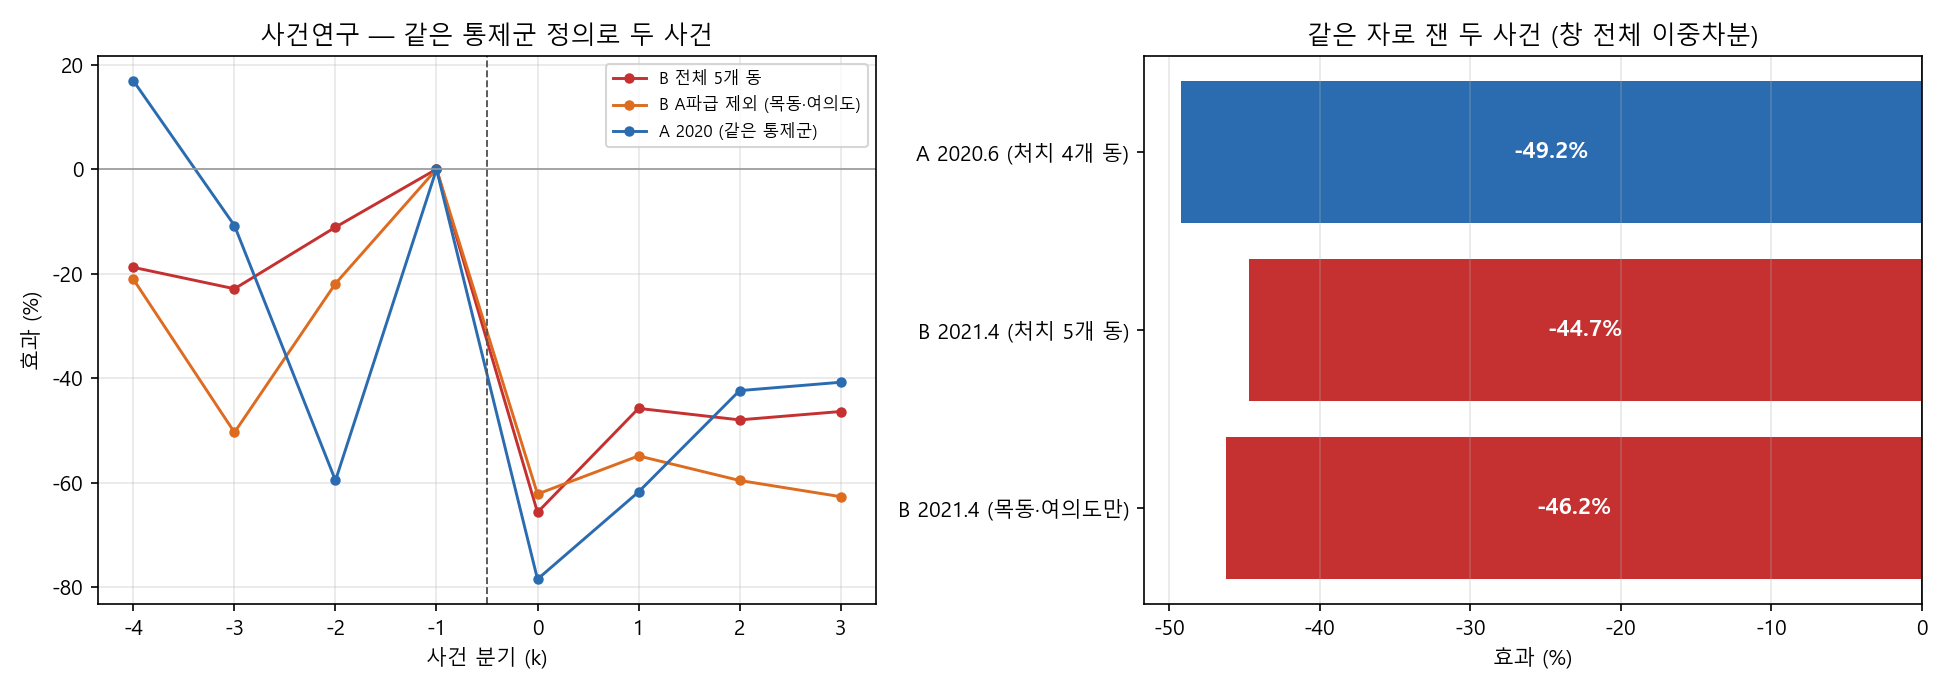
\includegraphics[width=\linewidth]{21_b_group.png}
  \caption{두 사건을 같은 자로. 왼쪽 사건연구, 오른쪽 창 전체 이중차분.}
  \label{fig:bgroup}
\end{figure}

\textbf{두 패널을 쌓아 차이를 직접 추정하면 $+8.7\%$, WCR $p$ 0.777, 무작위화
3{,}576/5{,}000($p=0.715$)다.} 0과 구분되지 않는다. \textbf{B가 A와 다르다고 할 수
없다.}

\textbf{덤으로 2.4절이 확인됐다.} A를 강남·송파 내부 통제로 재면 사건연구 $k=0$이
$-79.8\%$, 서울 전역 통제로 바꾸면 $-78.5\%$다. 사양 곡선이 통제군 축을 2.3\,\%p로
잰 것과 맞는다.

\textbf{면적 이질성은 B그룹에서 세울 수 없었다.} 2021년 지정의 허가 기준도 대지
18\,m$^2$이므로 메커니즘대로면 소형이 덜 줄어야 하고, 실제로 부호는 전부
양수다(40\,m$^2$에서 $+108.1\%$, $p=0.047$). 그러나 \textbf{40\,m$^2$ 미만 거래가
35건}(2020년은 322건)이고 경계를 올리면 유의성이 사라진다. 중위 전용면적은 A
84.8\,m$^2$ · B 85.0\,m$^2$로 같은데 40\,m$^2$ 미만 비중이 A 8.4\% 대 B
\textbf{1.2\%}다. \textbf{메커니즘의 반증이 아니라 검정력의 한계다.}

\textbf{B그룹 추정치를 주 결과로 올리지 않는다.} WCR이 0.057로 경계에 있고 기준분기
민감도도 A보다 넓다($-55.5 \sim -65.7\%$, 10\,\%p 폭 대 A의 7\,\%p). B는
\textbf{주 결과가 특정 지역의 산물이 아님을 보이는 보조 증거}다.

\subsection{자료 쪽 --- 취소거래}

마지막으로 \textbf{자료를 만들 때 뺀 것}이 결과를 바꾸는지 확인했다(0030).
3.3절에서 취소거래 6,293건을 뺐는데, 0004가 ``규제 직후에 몰린다면 그 자체가 정책
반응''이라는 숙제를 남겼었다.

% 자동 생성 — scripts/build_tables.py. 손으로 고치지 않는다.
% 출처: output/results/18_cancellations.json : 이중차분.2025-03-24 재지정
\begin{table}[htbp]
  \centering
  \caption{취소거래가 규제 직후에 몰리는가 (2025-03-24 재지정).}
  \label{tab:cancel}
  \begin{tabular}{lrrrrr}
    \toprule
    \textbf{창 (개월)} & \textbf{처치 전} & \textbf{처치 후} & \textbf{통제 전} & \textbf{통제 후} & \textbf{DID (\%p)} \\
    \midrule
    3 & 4.38 & 8.18 & 7.04 & 11.25 & -0.4 \\
    6 & 4.05 & 8.96 & 6.81 & 10.02 & +1.7 \\
    12 & 3.40 & 7.03 & 5.20 & 7.91 & +0.9 \\
    \bottomrule
  \end{tabular}

  \begin{minipage}{\linewidth}\footnotesize
  \textit{주.} 창을 바꾸면 부호가 바뀐다. 처치군 특유의 집중이 없다. 취소를 다시 넣어도 주 결과는 $0.3\%$p 움직인다.
  \end{minipage}
\end{table}


\begin{figure}[htbp]
  \centering
  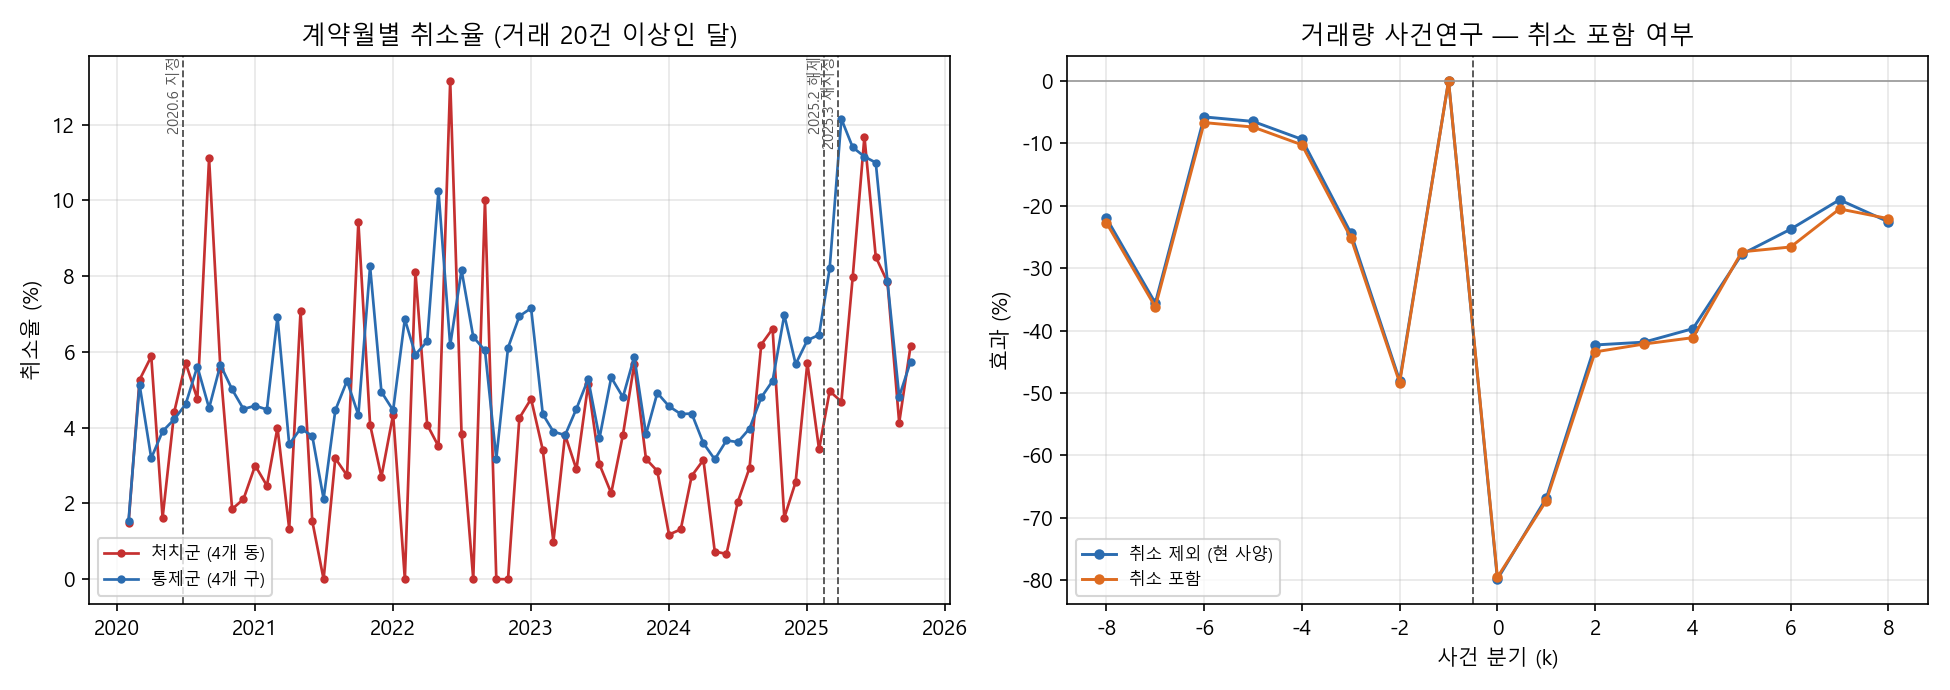
\includegraphics[width=\linewidth]{18_cancellations.png}
  \caption{취소거래의 시점별 분포. 왼쪽 계약월별 취소율, 오른쪽 취소를 넣은
           사건연구와 뺀 사건연구.}
  \label{fig:cancellations}
\end{figure}

\textbf{규제 직후에 몰리지 않는다.} 세 사건에 대해 취소율의 이중차분이 창에 따라
$-2.3 \sim +1.7$\,\%p로 부호가 바뀐다. 2025년에 양쪽 다 취소율이 오르는 것은 시장
전반의 일이고 처치와 무관하다.

\textbf{취소 거래가 더 비싸지도 않다.} 단지·계약월 고정효과 아래에서 취소 더미에
대한 $\log$ ㎡당가 회귀가 $-0.5\%$($p=0.443$)다. 허위신고 가설은 이 자료에서
지지되지 않는다.

\textbf{다시 넣어도 주 결과가 0.3\,\%p 움직인다}($-79.8 \to -79.5\%$). 취소율이
약 4\%이므로 사후 거래가 그만큼 깎이지만 \textbf{처치군과 통제군이 똑같이
깎이고} 이중차분은 공통된 비율 감소를 지운다.

\textbf{다만 취소 플래그는 2020년 2월 21일 계약분부터만 있다.} 2019년에 취소가
없었던 것이 아니라 자료에 없다. 이 비대칭을 처음에는 ``거래량 효과가 약 4\,\%p
부풀어 있다''고 적었다가, 재 보니 0.3\,\%p였다. \textbf{재지 않았으면 틀린 한계가
그대로 들어갔다.}

% 10장 논의. framing.md 2절 · 0022 · 0031

\section{논의}

\subsection{명분과 작동의 어긋남}

이 연구의 뼈대를 한 문장으로 쓰면 이렇다.

\begin{quote}
\textbf{토지거래허가제의 명분은 가격 안정인데 실제로 작동한 것은 거래
동결이었다.} 거래는 확실하게 끊었지만 가격을 잡았다는 증거는 약하다.
\end{quote}

이 어긋남은 두 숫자의 대비에 있다. 지정 직후 거래량은 반사실 대비
$-71 \sim -80\%$이고, 설계 조합 192가지 전부에서 음수이며, 사전 추세를 실제
관측값의 1.6배까지 열어 두어도 살아남고, 서로 다른 네 자치구에서 열 달 뒤에
일어난 별개 사건에서도 같은 크기다. 반면 가격은 평행추세를 가정해야 $-4 \sim
-7\%$이고 그 가정을 조금만 풀면 0과 구분되지 않으며 합성대조군으로는 확인되지
않는다.

\textbf{이것은 제도가 실패했다는 말이 아니다.} 제도가 직접 건드리는 것은 거래가
성립하는 절차이지 가격이 아니므로, 거래가 멈춘 것은 제도의 설계대로 작동한
결과다. 말할 수 있는 것은 \textbf{그 작동이 명분까지 닿았다는 증거가 이 자료에서
나오지 않는다}는 것이다.

\subsection{설계 세부가 효과를 가른다 --- 정책 시사점}

\textbf{이 연구의 가장 실용적인 결론은 6장에 있다.}

2020년 지정의 허가 대상은 주거지역 대지 \textbf{18\,m$^2$ 초과}였다. 그 선 아래의
소형 아파트는 구역 안에 있어도 허가 없이 거래할 수 있었고, 실제로 거래가 줄지
않았다 --- 줄지 않은 정도가 아니라 \textbf{통제군 대비 두 배 이상으로 늘었다}
($+125.7\%$). 규제가 수요를 없앤 것이 아니라 \textbf{면제 구간으로 밀어냈다.}

2022년 6월 23일 그 기준이 \textbf{6\,m$^2$}로 좁아졌다. 그러자 \emph{그때} 소형
거래가 약 3분의 1 줄었고($-33.2\%$), 기준을 바꾸지 않은 2021년 재지정에서는
움직이지 않았다($-8.1\%$).

\begin{quote}
\textbf{규제를 ``거느냐 마느냐''가 아니라 ``어떻게 거느냐''가 효과를 정한다.}
가격 차등(대출 규제)보다 설계 세부(허가 대상의 면적 기준)가 규제의 실효를 갈랐다.
\end{quote}

이 결론에는 두 가지 함의가 있다.

\textbf{첫째, 면적 기준이 사실상의 회피 통로였다.} 규제를 피할 수 있는 물건은
거래가 유지됐고 통로가 닫히자 줄었다. 제도 설계자가 2년 뒤 기준을 6\,m$^2$로
고친 것은 규제 당국도 결국 같은 것을 알아챘음을 시사한다.

\textbf{둘째, 정책 평가가 평균만 보면 이 사실이 보이지 않는다.} 동 평균 안에서
대형의 $-95\%$와 소형의 $+126\%$가 상쇄되어 하나의 숫자로 뭉개진다. 거래마다
전용면적이 붙은 미시 자료가 아니면 \textbf{애초에 볼 수 없다.} 선행연구 세 편이
동 단위 집계로 ``60\% 줄었다''에서 멈춘 이유가 여기 있다.

\subsection{거래 동결 자체가 비용이다}

``거래가 줄었다''를 중립적인 사실로 읽으면 안 된다. 거래가 80\% 끊기면 이사가
필요한 사람도 옮기지 못하고, 시장이 값을 찾는 신호도 약해진다. \textbf{효과의
크기와 지속을 재는 일은 그 비용을 재는 일이기도 하다.}

그래서 ``언제까지 갔나''가 중요한 질문이었고, \textbf{이 연구는 그 질문에
답하지 못했다}(다음 절).

\subsection{한계}

숨기지 않고 적는다.

\textbf{일반화의 범위.} 처치가 두 사건·아홉 개 동이고 \textbf{두 집단 모두 서울
고가 재건축 지역}이다. 2021년 B그룹에서 같은 크기의 효과가 나왔고 두 사건의
차이가 0과 구분되지 않았지만(9.6절), 완전히 다른 유형의 지역은 아니다.
\textbf{``서울 고가 재건축 지역에서는 일관된다''까지가 정확하고}, 지방이나 다른
유형의 지역에는 말할 수 없다.

\textbf{지속 기간을 말할 수 없다.} 사후 $k \geq 4$는 기준 분기 선택에 따라
$-20 \sim +16\%$로 흔들리고, 24개월 평균의 붕괴값이 0.05이며, 합성대조군에서
사후 27개월 평균은 152개 중 22위($p=0.145$)다. 세 진단이 같은 방향을 가리킨다.
\textbf{일시 충격인지 지속적 동결인지는 이 설계로 답할 수 없다.}

\textbf{가격의 크기를 말할 수 없다.} 방향까지만 쓴다(8.6절).

\textbf{부과와 해제의 대칭성을 가릴 수 없다.} $\text{DID}_M$에서 부과 쪽은 구간이
0을 품지 않고 해제 쪽은 품는다(9.4절).

\textbf{대출의 몫을 가릴 수 없다.} 면적 기준이 주된 원인이라는 것이 대출의 몫이
0이라는 뜻은 아니다. 소형을 뺀 뒤에도 15억 경계의 차이가 점추정으로 남는다
(무작위화 $p=0.098$). 폐지를 사건으로 걸어 한 번 더 시도했으나 금리 정점 통과와
1·3 대책에서 가를 수 없었다(6.9절).

\textbf{대지지분이 자료에 없다.} 허가 기준은 대지지분인데 실거래 자료에 없어
전용면적으로 대신했다. 2021년 B그룹에서 더 부정확하다 --- 1970$\sim$80년대 재건축
대상 단지라 용적률이 낮아 같은 전용면적이라도 대지지분이 클 수 있다. B그룹 소형
검정이 방향만 맞고 세워지지 않은 이유의 하나다.

\textbf{거래 주체를 보지 못했다.} 법인 매수와 직거래 비중은 규제 회피 경로를
직접 가리키는 변수인데, \texttt{dealingGbn}이 2021년 말, \texttt{slerGbn}·
\texttt{buyerGbn}이 2024년부터 채워져 \textbf{2020·2021 사건에는 원천적으로 쓸 수
없다}(2020년은 12개월 전부 결측). 2025년 사건에만 적용 가능하다.

\textbf{취소 플래그가 2020년 2월부터다.} 사건연구 사전 구간의 대부분에서 취소를
뺄 수 없고 사후에서는 뺀다. 재 보니 그 비대칭이 주 결과를 0.3\,\%p 움직인다
(9.7절).

\textbf{저장소가 무겁다.} 그림을 매번 커밋해 \texttt{.git}이 936\,MB다. 이력을
다시 쓰는 일이라 이번 학기에는 고치지 않았다.

% 11장 결론. 세 문장으로 끝낸다.

\section{결론}

\textbf{첫째, 토지거래허가제는 거래를 확실하게 멈췄다.} 2020년 6월 지정 직후
3개월 거래량이 반사실 대비 $-71 \sim -80\%$다. 법정동 27개 가운데 4개를 처치로
고르는 17,550가지 중 진짜 배정이 1위이고, 사전 추세 위배를 실제 관측값의
1.6배까지 열어 두어도 구간이 0을 넘지 않으며, 합리적인 설계 조합 192가지가 전부
음수다. 완전히 다른 네 자치구에서 열 달 뒤에 일어난 2021년 지정에서도 같은
크기였고 두 사건의 차이는 0과 구분되지 않았다($p=0.715$).

\textbf{둘째, 그러나 모두에게 같지 않았고 그 차이는 제도 설계의 세부에서 왔다.}
2020년 지정은 대지 18\,m$^2$ 초과만 허가 대상이어서 소형 아파트는 거래가 줄지
않았다 --- 줄지 않은 정도가 아니라 통제군 대비 두 배 이상으로 늘었다. 2022년 6월
그 기준이 6\,m$^2$로 좁아지자 \emph{그때} 소형이 3분의 1 줄었고, 기준을 바꾸지
않은 2021년 재지정에서는 움직이지 않았다. 이 메커니즘에서 세운 예측 ---
``면적 기준이 6\,m$^2$인 2025년 재지정에서는 소형도 함께 줄어야 한다'' --- 이
결과를 보기 전에 기록되었고 자료에서 확인됐다(소형 $-71.5\%$).
\textbf{규제를 거느냐가 아니라 어떻게 거느냐가 효과를 정한다.}

\textbf{셋째, 가격을 잡았다는 증거는 약하다.} 평행추세를 가정하면 $-4 \sim -7\%$
이나 그 가정을 조금만 풀면 0과 구분되지 않고(붕괴값 0.22) 합성대조군으로도
확인되지 않는다($p=0.511$). 제도의 명분은 가격 안정인데 실제로 작동한 것은 거래
동결이었다. \textbf{이 어긋남을 숫자로 보인 것이 이 연구의 결론이다.}

\vspace{1em}

말할 수 없는 것도 함께 남긴다. 효과가 얼마나 오래 갔는지, 부과와 해제가 대칭인지,
대출 규제의 몫이 얼마인지는 이 설계로 답할 수 없다. \textbf{걸어 봤으나 가릴 수
없었다는 것도 결과이며}, 걸어 보지 않았으면 그 사실조차 몰랐을 것이다.

이 보고서의 또 하나의 축은 \textbf{분석의 전제가 되는 시스템}이었다. 원자료
수집부터 그림과 표 생성까지 48단계 파이프라인 하나로 돌고, 문서의 숫자가 분석
결과와 어긋나지 않는지·아무도 만들지 않는 산출물이 남아 있지 않은지·의존 목록이
실제 \texttt{import}와 맞는지를 매 실행마다 점검한다. 새 폴더에 내려받아 새
가상환경에서 돌려 결과 파일 25개가 바이트 단위로 같은 것을 확인했다. 그 과정에서
의존 목록의 구멍 둘과 석 달 묵은 유령 숫자를 찾았다.

\textbf{미시 자료로 내려간 것 자체가 기여는 아니다.} 기여는 미시 자료가 아니면
보이지 않는 것을 보였다는 데 있고, 면적 기준 발견이 그 주장의 가장 좋은 증거다.
동 평균 안에서 대형의 $-95\%$와 소형의 $+126\%$는 하나의 숫자로 뭉개진다.
\textbf{제목의 두 층 --- 미시 패널 구축과 인과효과 추정 --- 이 만나는 지점이
여기다.}


% 본문에서 실제로 인용한 것만 싣는다. 인용하지 않은 항목은 references.bib 에
% 남아 있되 출력되지 않는다.
\bibliographystyle{apalike}
\bibliography{references}

\appendix
% 부록. 결정기록 색인 · 재현 절차 · 선행연구 재현 상세

\section{결정기록}

설계를 정할 때마다 왜 그렇게 정했는지를 한 편씩 남겼다. 근거와 함께
\textbf{버린 대안}도 적는다. 본문에서 ``0014''와 같이 가리키는 것이 이 번호이며,
전문은 저장소의 \texttt{docs/decisions/}에 있다.

% 자동 생성 — scripts/build_tables.py. 손으로 고치지 않는다.
% 출처: docs/decisions/*.md
\begin{table}[htbp]
  \centering
  \caption{결정기록. 설계를 정할 때마다 왜 그렇게 정했는지를 한 편씩 남겼고 근거와 함께 \textbf{버린 대안}도 적었다.}
  \label{tab:decisions}
  \begin{tabular}{llp{9.5cm}}
    \toprule
    \textbf{번호} & \textbf{날짜} & \textbf{제목} \\
    \midrule
    0001 & 09-03 & 주 결과변수를 가격에서 거래량으로 변경 \\
    0002 & 09-03 & 분석 구간을 2025-10-19 이전으로 한정 \\
    0003 & 09-03 & 단지(aptSeq) 고정효과를 기본 사양으로 채택 \\
    0004 & 09-03 & 취소거래 제외 및 신고지연 절단 \\
    0005 & 09-03 & 처치 역전 구간에 de Chaisemartin \& D'Haultfœuille 추정량 사용 \\
    0006 & 09-03 & 모든 결과를 반사실 대비로 명시하여 서술한다 \\
    0007 & 09-07 & 문서를 동결·살아있는·최종으로 나누고, 숫자에 조건을 붙인다 \\
    0008 & 09-07 & 지정 유지 단지를 단지명이 아니라 지번으로 확정한다 \\
    0009 & 09-07 & 통제군 오염 점검 결과와 대응 \\
    0010 & 09-07 & 2020년 지정 범위를 법정동 단위 처치로 확정한다 \\
    0011 & 09-08 & 통제군을 어떻게 고르는가 \\
    0012 & 09-08 & 처치군을 무엇으로 하고, 무엇을 확장으로 미루는가 \\
    0013 & 09-11 & 사건 시점을 효력일에 맞추고, 거래 없는 달을 0으로 채운다 \\
    0014 & 09-11 & 거래량의 사전 추세 위배를 어떻게 다루는가 \\
    0015 & 09-11 & 대출 규제를 어떻게 다루는가 — 무엇이 상쇄되고 무엇이 남는가 \\
    0016 & 09-11 & 위약 검정 — 효과는 있으나 크기는 구간으로 말한다 \\
    0017 & 09-11 & 합성대조군 — 평균 회귀 의심에 답한다 \\
    0018 & 09-11 & 반복매매지수를 어떻게 짓는가 \\
    0019 & 09-18 & 클러스터가 적을 때의 추론 — 관행 p 를 버린다 \\
    0020 & 09-18 & 오염 동을 빼도 직후 효과는 그대로이고, 24개월 효과는 커진다 \\
    0021 & 09-18 & 15억에는 계단이 없다 — 가격 차이는 면적 면제와 겹친다 \\
    0022 & 09-18 & 이질성은 대출이 아니라 허가 면적 기준에서 왔다 \\
    0023 & 09-23 & 2025년 구간은 해제가 아니라 재지정으로 본다 \\
    0024 & 09-23 & 파급은 같은 동 안에만 있었다 — '인근 급등'은 기준점이 만든 말이다 \\
    0025 & 09-23 & 가격 효과는 −4 \textasciitilde{} −7\% 로 모인다 — 다만 합성대조군으로는 확인되지 않는다 \\
    0026 & 09-30 & 사전 추세를 감안하면 직후 거래량만 남는다 \\
    0027 & 09-30 & 음의 가중치는 작다 — 부과는 뚜렷하고 해제는 가릴 수 없다 \\
    0028 & 09-30 & 192개 사양 전부 음수다 — 갈린 것은 통제군이 아니라 날짜 세는 법이었다 \\
    0029 & 10-01 & 폐지 뒤 고가 거래는 돌아왔지만 그 규제 덕으로 돌릴 수 없다 \\
    0030 & 10-01 & 취소거래는 정책 반응이 아니다 — 그리고 0004 의 한계는 생각보다 작다 \\
    0031 & 10-08 & 강남·송파 밖에서도 같다 — B그룹이 A그룹과 다르다고 할 수 없다 \\
    \bottomrule
  \end{tabular}

  \begin{minipage}{\linewidth}\footnotesize
  \textit{주.} 날짜는 \textbf{작성일}이다 --- 뒤에 보강·정정된 기록이 있다. \textbf{이 표는 \texttt{docs/decisions/}의 파일들에서 생성된다.} 손으로 적었을 때는 색인의 날짜 셋이 정작 그 기록과 달랐다.
  \end{minipage}
\end{table}


\textbf{결정이 바뀐 것도 지우지 않고 그 자리에 정정으로 남겼다.} 0001의 근거 2는
2026-09-11에, 0004의 수치와 한계는 2026-10-01과 10-15에, 0015의 이질성 결론은
0021과 0022에서 바뀌었다. 바뀐 과정 자체가 이 연구의 기록이다.

\section{자료 출처와 이용 조건}

이 연구의 자료는 전부 공개 자료이며, 저장소를 공개하기 때문에 \textbf{무엇을
넣었고 무엇을 뺐는지}를 밝혀 둔다.

\begin{itemize}[leftmargin=2em, itemsep=3pt]
  \item \textbf{아파트 매매 실거래 상세 자료} --- 국토교통부, 공공데이터포털
        (\texttt{data.go.kr}) 오픈 API \texttt{RTMSDataSvcAptTradeDev}.
        활용신청 승인 뒤 이용했다. \textbf{인증키는 저장소에 넣지 않는다} ---
        \texttt{.env}(git 제외)에서 읽고 저장소에는 \texttt{.env.example}만 둔다.
        내려받은 원자료 902\,MB도 저장소 밖이다.
  \item \textbf{토지거래허가구역 지정·해제 공고} --- 서울특별시 \emph{서울시보}와
        전자관보에 실린 공고 원문. 누구나 열람할 수 있는 공보이며, 이 연구가 쓴
        공고 번호는 본문과 \texttt{data/policy/ltz\_events.csv}에 적었다.
        서울시보 원본(2.9\,GB)은 용량 때문에 저장소 밖에 두고 \textbf{해당
        공고만 발췌한 PDF}를 저장소에 넣었다.
  \item \textbf{행정구역 경계} --- 법정동 폴리곤. 맞닿은 동 판정(7장)에만 쓴다.
  \item \textbf{선행연구 논문} --- \textbf{저장소에 넣지 않았다.} 학술지 논문은
        저작권이 있으므로 개인적으로 내려받아 읽었을 뿐이며, 재현 코드
        (\texttt{scripts/replicate/})와 \textbf{논문이 보고한 수치만} 저장소에
        있다. 재현에는 원문 PDF가 필요하지 않다.
\end{itemize}

\textbf{개인정보는 다루지 않는다.} 실거래 자료는 단지·면적·층·계약일·금액만
담고 거래 당사자를 식별하는 정보가 없다. 가장 작은 분석 단위가
\textbf{(단지, 전용면적, 층)}이며 이는 특정 호실이 아니다(3.4절).

\section{재현 절차}

\subsection{전체 실행}

\begin{verbatim}
pip install -r requirements.txt
cp .env.example .env          # 공공데이터포털 Decoding 키 입력
python run_all.py --collect   # 수집부터 전부 (수십 분)
python run_all.py             # 수집 생략, 정제부터 문서까지 전부 (약 21분)
python run_all.py --list      # 전체 단계 목록
\end{verbatim}

\subsection{클린 환경에서 재현할 때}

새 폴더에 내려받아 새 가상환경에서 돌려 \texttt{output/results/*.json} 25개가
바이트 단위로 같은 것을 확인했다(2026-10-15). 그때 걸린 것 셋을 적어 둔다.

\textbf{첫째, \texttt{data/raw}는 git 밖이다}(902\,MB). \texttt{--collect}로 다시
받으면 \textbf{같은 결과가 나오지 않는다} --- 실거래 자료가 소급 갱신되기
때문이다. 재현하려면 \textbf{같은 스냅샷을 복사}해 와야 한다. 현재 스냅샷은
\textbf{2026-09-03 수집}이다.

\textbf{둘째, 경로가 길면 설치가 깨진다.} 윈도 기본 한계가 260자인데
\texttt{statsmodels}의 시험 자료 경로가 깊어 넘어간다. 137자짜리 폴더에서 266자가
되어 \texttt{statsmodels}만 빠진 채 설치가 끝났다. 짧은 경로에 두거나 긴 경로
지원을 켠다.

\textbf{셋째, 소요 시간.} \texttt{pip install} 약 12분, \texttt{run\_all.py} 약
21분.

\subsection{최종 보고서 빌드}

\begin{verbatim}
winget install --id MiKTeX.MiKTeX --scope user
.\paper\build.ps1
\end{verbatim}

\textbf{그림은 하나도 복사하지 않는다} --- \texttt{output/figures}를 그대로
참조하므로 분석을 다시 돌리면 보고서의 그림이 따라 바뀐다. 표는 전부가 아니라
\textbf{수치가 결과 JSON에 있는 \pipeTables 개}를
\texttt{scripts/build\_tables.py}가 생성한다
(\texttt{paper/tables/*.tex}). 나머지 표는 설계 비교·제도 요약처럼 분석 산출물이
아닌 것을 담으므로 본문에 직접 적었다. \textbf{손으로 적은 표에 분석 수치를
넣지 않는 것}이 경계선이다.

\section{선행연구 재현 상세}

\texttt{scripts/replicate/}에 전상현 외(2025)와 이한웅·이춘원(2025)의 사양을
복제한 코드가 있다. 본문 2.3절의 요약을 뒷받침하는 수치는 다음과 같다.

\begin{table}[htbp]
  \centering
  \caption{전상현 외(2025) 재현 --- 빈 셀 처리에 따라 교호항 부호가 바뀐다}
  \label{tab:replicate-jeon}
  \begin{tabular}{lrrrrr}
    \toprule
    \textbf{사양} & \textbf{Zone} & \textbf{Time} & \textbf{Zone\#Time} &
    \textbf{거래건수} & \textbf{$R^2$} \\
    \midrule
    논문 보고값 & $+0.3263$ & $+0.2724$ & $+0.2928$ & $+0.0116$ & 0.0757 \\
    빈 셀 0 코딩 ($N=675$) & $+0.3464$ & $+0.2334$ & $+0.3549$ & $+0.0138$ &
      0.0804 \\
    \textbf{빈 셀 제외} ($N=644$) & $+0.3038$ & $+0.1964$ &
      $\mathbf{-0.0448}$ & $+0.0023$ & 0.2496 \\
    \bottomrule
  \end{tabular}
\end{table}

빈 셀 31개는 전부 통제동(삼전·석촌·압구정·율현)이다. 거래건수를 통제에서 빼면
교호항이 $-0.1121$($p=0.002$), 동·월 고정효과까지 넣으면 $-0.1215$가 된다.

\begin{table}[htbp]
  \centering
  \caption{이한웅·이춘원(2025) --- 논문 표의 수치로 차이의 차이를 계산하면}
  \label{tab:replicate-lee}
  \begin{tabular}{lrrr}
    \toprule
    \textbf{창} & \textbf{잠실} & \textbf{비잠실} & \textbf{차이의 차이} \\
    \midrule
    $\pm$3개월 & $+16.5\%$ & $+4.3\%$ & $+12.2$\,\%p \\
    $\pm$6개월 & $+9.6\%$ & $+12.5\%$ & $\mathbf{-2.9}$\,\%p \\
    $\pm$12개월 & $+19.0\%$ & $+22.9\%$ & $\mathbf{-3.9}$\,\%p \\
    \bottomrule
  \end{tabular}
\end{table}

논문이 보고한 $t$-검정은 각 집단 \textbf{내부}의 사전-사후 비교이며 이중차분
계수가 아니다. 잠실동 가격이 유의하게 올랐다는 것은 맞지만 통제동도 함께, 그리고
$\pm$6개월부터는 더 많이 올랐다.


\end{document}
